%!TEX encoding = UTF-8 Unicode
%!TEX program = xelatex

\documentclass[doctor]{hnuthesis}
\usepackage{subfigure}
\usepackage{amsmath}
\usepackage{algorithmicx,algpseudocode}
\graphicspath{{figures/}}

% 学校代码
\hnucode{10532}
% 学校名称
\hnuname{湖南大学}
\enhnuname{Hunan University}
% 中图分类号
\clc{TP391}         
% 密级       
\secrettext{普通}           

% 标题
\title{基于多核系统的并发哈希表的设计与应用研究}
\entitle{TODO}  
% 作者
\author{陈志文}
\enauthor{ZHIWEN Chen}
% 学号
\authorid{B1310S0004}      
% 学院
\college{信息科学与工程学院}
% 专业
\major{计算机科学与技术} 
\enmajor{Computer Science and Technology}

%\enbachelor{B.E.~(Hunan University)2004}
\enmaster{M.S.~(Hunan University)2013}
\endoctor{Doctor of engineering}
% 研究方向
\workon{高性能计算}
% 导师
\supervisor{陈浩\ 教授}
\ensupervisor{Professor HAO Chen}
% 论文提交、答辩日期
\submitdate{二〇一七年七月二十日}
\defensedate{二〇一七年七月二十日}
\endate{May, 2013}
% 答辩委员会主席
\chair{待定}

\begin{document}
% 封面、原创性声明
\maketitle

% 摘要
%%!TEX root =  ../main.tex

\begin{abstract}
	随着多处理器技术的日臻成熟以及集成到单个处理器上的处理器核心数量的日趋增加,计算机的运算能力的瓶颈不断被打破,同时这也为设计具有高可扩展性的并发数据结构以及开发基于多核架构的高性能软件系统提出了挑战。
    并发哈希表是一种重要的并发数据结构,因其处理元素的开销为常数时间的特性被广泛应用于多核架构的软件系统开发。
    在并发哈希表的设计、优化以及应用中,处理器的体系结构,缓存一致性协议,内存带宽,内存访问延迟以及多线程的同步机制都对其性能产生重大影响。
    本文针对基于多核系统的并发哈希表做了如下工作:


    首先,设计了用于并发哈希表的测试、评估的统一测试框架 CHTBench。 
    CHTBench是目前第一个用于并发哈希表性能比较与评估的,能保证测试结果公平性与客观性的测试框架。
    它提供统一的测试接口,具有可配置的线程与核的映射关系,能够测试不同规模的数据集以及数据集中更新操作的比重等。
    此外,CHTBench使用$sspfd$进行延迟的测算,综合考察不同并发哈希表线程扩展性,查询和更新吞吐量等宏观指标。结合其它的工具,如$likwid$ 对缓存命中率,内存带宽,跨内存节点通信开销等微观指标进行分析以及$sspfd$对各种操作类型的延迟进行比较。
    使用CHTBench 可以为并发哈希表的评估和比较提供相对公平的测试环境。

    第二,基于CHTBench测试框架对现有的几种具有代表性的并发哈希表在四个不同的多核系统上进行了深入的剖析。对并发哈希表的评估选用的性能指标涵盖宏观和微观两个层面,包括吞吐量的线程扩展性,延迟,分层内存结构对性能的影响,不同线程与核映射方式之间的性能差异,同步机制的性能评估以及内存消耗。通过对上述指标的分析,找出现有并发哈希表设计方法中存在的问题以及可能的性能瓶颈,分析总结了8条设计、优化并发哈希表的最佳实践原则,为将来进一步设计基于多核系统的、具有高可扩展性的并发哈希表奠定理论和实践基 础。根据对比现有文献以及相关研究工作,我们对于并发哈希表的评估所用的方法和涉及的评估指标是迄今为止最全面的。

    第三,使用Intel限制性事务内存(RTM)实现了基于硬件事务内存的缓存行哈希表。使用全局锁实现了基于RTM的缓存行哈希表。实验评估结果表明,当数据集的规模大于最后一级缓存容量时,基于RTM的缓存行哈希表的性能是使用传统的细粒度锁方法实现的缓存行哈希表的120\%。使用硬件事务内存进行并发哈希表的设计真正做到了粗粒度锁方法的简便与细粒度锁方法的高性能的有机结合。同时,为了消除Intel TSX的Lemming效应对性能的影响,设计了两种软件辅助方法:软件辅助的锁省略方法(SLR)和软件辅助的冲突管理方法(SCM)。实验结果表明,这两种方法对基于RTM的缓存行哈希表性能的提升比使用Intel官方推荐的RTM Retry机制更明显。

最后,使用不完整键Cuckoo哈希方法设计并实现了支持多线程并发的
Cuckoo过滤器。这是迄今为止第一款支持多线程并发的过滤器实现,同时也是第一款基于硬件事务内存的过滤器。
原始的布隆过滤器不支持删除操作,实现删除操作需要引入额外的空间开销,通过使用不完整键Cuckoo哈希方法,通过哈希函数生成指纹,利用Cuckoo哈希表多路组相连能够存储多个相同的指纹信息的特点实现了删除操作,不额外增加过滤器的空间开销。使用基于Intel RTM的读写锁实现了多线程并发的Cuckoo过滤器。实验评估表明,并发Cuckoo过滤器的初始化速度是使用单个线程初始化的10倍,查询操作的性能是单个线程的38 倍,处理更新占10\%的数据集的性能是单个线程的11倍。此外,还对retry的最大值如何选取以及使用不同软件优化方法的Cuckoo 过滤器版本进行了线程扩展性的比较。

    
  	\keywords{多核系统;缓存一致性;并发哈希表;布隆过滤器;同步;非一致性内存架构;硬件事务内存}
\end{abstract}

\begin{enabstract}
	 As the development of multi-processor techniques and the increasing of the number of cores integrated into a single CPU chip the bottleneck of computing power of the processor is constantly being broken. 
	 It also makes designing highly scalable concurrency data structures and developing high-performance software systems based on multi-core architectures more complicated.
	 Concurrent hash table(CHT) is an important concurrent data structure and it is widely used to implement software systems on multi-core architectures as its queries run in amortized constant time.
	 The hardware architecture, cache coherence protocol, memory bandwidth, memory access latency and multi-thread synchronization mechanism impact the designing, optimization and application of CHT significantly.
     The works of this paper including:

     First, we present a framework, named CHTBench, which provides a fair testing environment and unified interface for the experiments by hiding the discrepancies of hardware platforms, synthesized workloads, concurrency models, and compiler configurations. 
     In this way, we can guarantee the experimental results generated from our framework are fairly comparable between different CHTs. 
     An open source library, $sspfd$, is integrated into CHTBench to measure the access latency of different kinds of operations.
     With CHTBench it's easy to compare the performance of CHTs. And it can also combine with other system tools such as $likwid$ to measure cache hit/miss rate, memory bandwidth overheads and cross-socket node communication overheads from micro perspective.
    
     Second, we dissected 5 state of the art CHTs on CHTBench. The evaluations are explored from a wide range of perspectives including thread scalability, throughput, latency, memory hierarchy impact, low-level synchronization primitives, and memory usage. The inter-correlations between relevant metrics are also discussed when necessary. The experiments are conducted on four major hardware platforms including Intel Many Integrated Core(MIC) architecture and three representative Non-uniform Memory Architecture(NUMA) systems. We ported CHTs to the MIC platform, and to our knowledge, this is the first extensive study of concurrent hash tables on Intel MIC architecture. 
     According to the experimental results, Œeight principles of best practices in designing and optimizing concurrent hash tables are summarized which lay the theoretical and practical foundation for further design of high scalability concurrent hash tables based on multi-core systems in the future. 


    Then, inspired by the fine-grained Cache Line Hash Table, we implemented a concurrent cache-line hash table with hardware transactional memory(HTM-CLHT).
    The size of a HTM-CLHT bucket is padding to the size of cache line(64 bytes in our testbed). 
    The HTM-CLHT takes the whole hash table as the critical section which can provides optimistic concurrenty control by allowing threads to run in parallel with minimal interference.
    When running workloads which large than the capacity of LLC, the performance of HTM-CLHT is twenty percent better than using traditional fine-grained locks. 
    HTM-CLHT achieves the goal that using a simple, coarse-grained locking method, obtaining high performance which matched with sophisticated synchronization methods such as fine-grained locking and non-blocking.  
   In order to eliminate the Lemming effect of Intel TSX, we presented two software-assisted techniques, lock removal(SLR) and conflict management(SCM).
    Both of these methods improve the performance of the HTM-based concurrent hash table more significantly than the RTM Retry mechanism recommended by Intel.

    At last, we presented a concurrent Cuckoo Filter based on partial-key Cuckoo Hashing.
    To our knowledge, this is the only concurrent filter so far, and its also the only one which based on hardware transactional memory(HTM).
    The standard Bloom Filter do not support delete elements from filter, while other extended versions of Bloom Filter support the deletion of filters with high space overheads.
    The structure of Cuckoo Hashing is in a set-associative way, each element can map to several slots.
    Taking this feature of Cuckoo hash table, we extract the fingerprints of the members of a set and store them in a hash table. 
    And items with same fingerprint are fine, i.e. the filter can store several identical fingerprint.
    To delete an item from Cuckoo Filter, the fingerprint of this item is deleted from filter.
    If there is another item has the same fingerprint, we can still find this item with a copy of this fingerprint.
    This can delete an element very easy and straightforward without any additional space overheads.
    According to our experiment results, when running with read-only workloads, the max throughput is 38 times of the throughput of a single thread, and running workloads with ten percent update operations, the max throughput is 11 times of the throughput running workload with a single thread.

  	\enkeywords{Multi-core System; Cache Coherence; Concurrent Hash Table; Synchronization; Non-uniform Memory Architecture; Hardware Transactional Memory}
\end{enabstract}
% 目录
\tableofcontents
% 插图附表索引
\listoffigures
\listoftables

% 正文章节
\mainmatter
% %!TEX root =  ../main.tex

\begin{abstract}
	随着多处理器技术的日臻成熟以及集成到单个处理器上的处理器核心数量的日趋增加,计算机的运算能力的瓶颈不断被打破,同时这也为设计具有高可扩展性的并发数据结构以及开发基于多核架构的高性能软件系统提出了挑战。
    并发哈希表是一种重要的并发数据结构,因其处理元素的开销为常数时间的特性被广泛应用于多核架构的软件系统开发。
    在并发哈希表的设计、优化以及应用中,处理器的体系结构,缓存一致性协议,内存带宽,内存访问延迟以及多线程的同步机制都对其性能产生重大影响。
    本文针对基于多核系统的并发哈希表做了如下工作:


    首先,设计了用于并发哈希表的测试、评估的统一测试框架 CHTBench。 
    CHTBench是目前第一个用于并发哈希表性能比较与评估的,能保证测试结果公平性与客观性的测试框架。
    它提供统一的测试接口,具有可配置的线程与核的映射关系,能够测试不同规模的数据集以及数据集中更新操作的比重等。
    此外,CHTBench使用$sspfd$进行延迟的测算,综合考察不同并发哈希表线程扩展性,查询和更新吞吐量等宏观指标。结合其它的工具,如$likwid$ 对缓存命中率,内存带宽,跨内存节点通信开销等微观指标进行分析以及$sspfd$对各种操作类型的延迟进行比较。
    使用CHTBench 可以为并发哈希表的评估和比较提供相对公平的测试环境。

    第二,基于CHTBench测试框架对现有的几种具有代表性的并发哈希表在四个不同的多核系统上进行了深入的剖析。对并发哈希表的评估选用的性能指标涵盖宏观和微观两个层面,包括吞吐量的线程扩展性,延迟,分层内存结构对性能的影响,不同线程与核映射方式之间的性能差异,同步机制的性能评估以及内存消耗。通过对上述指标的分析,找出现有并发哈希表设计方法中存在的问题以及可能的性能瓶颈,分析总结了8条设计、优化并发哈希表的最佳实践原则,为将来进一步设计基于多核系统的、具有高可扩展性的并发哈希表奠定理论和实践基 础。根据对比现有文献以及相关研究工作,我们对于并发哈希表的评估所用的方法和涉及的评估指标是迄今为止最全面的。

    第三,使用Intel限制性事务内存(RTM)实现了基于硬件事务内存的缓存行哈希表。使用全局锁实现了基于RTM的缓存行哈希表。实验评估结果表明,当数据集的规模大于最后一级缓存容量时,基于RTM的缓存行哈希表的性能是使用传统的细粒度锁方法实现的缓存行哈希表的120\%。使用硬件事务内存进行并发哈希表的设计真正做到了粗粒度锁方法的简便与细粒度锁方法的高性能的有机结合。同时,为了消除Intel TSX的Lemming效应对性能的影响,设计了两种软件辅助方法:软件辅助的锁省略方法(SLR)和软件辅助的冲突管理方法(SCM)。实验结果表明,这两种方法对基于RTM的缓存行哈希表性能的提升比使用Intel官方推荐的RTM Retry机制更明显。

最后,使用不完整键Cuckoo哈希方法设计并实现了支持多线程并发的
Cuckoo过滤器。这是迄今为止第一款支持多线程并发的过滤器实现,同时也是第一款基于硬件事务内存的过滤器。
原始的布隆过滤器不支持删除操作,实现删除操作需要引入额外的空间开销,通过使用不完整键Cuckoo哈希方法,通过哈希函数生成指纹,利用Cuckoo哈希表多路组相连能够存储多个相同的指纹信息的特点实现了删除操作,不额外增加过滤器的空间开销。使用基于Intel RTM的读写锁实现了多线程并发的Cuckoo过滤器。实验评估表明,并发Cuckoo过滤器的初始化速度是使用单个线程初始化的10倍,查询操作的性能是单个线程的38 倍,处理更新占10\%的数据集的性能是单个线程的11倍。此外,还对retry的最大值如何选取以及使用不同软件优化方法的Cuckoo 过滤器版本进行了线程扩展性的比较。

    
  	\keywords{多核系统;缓存一致性;并发哈希表;布隆过滤器;同步;非一致性内存架构;硬件事务内存}
\end{abstract}

\begin{enabstract}
	 As the development of multi-processor techniques and the increasing of the number of cores integrated into a single CPU chip the bottleneck of computing power of the processor is constantly being broken. 
	 It also makes designing highly scalable concurrency data structures and developing high-performance software systems based on multi-core architectures more complicated.
	 Concurrent hash table(CHT) is an important concurrent data structure and it is widely used to implement software systems on multi-core architectures as its queries run in amortized constant time.
	 The hardware architecture, cache coherence protocol, memory bandwidth, memory access latency and multi-thread synchronization mechanism impact the designing, optimization and application of CHT significantly.
     The works of this paper including:

     First, we present a framework, named CHTBench, which provides a fair testing environment and unified interface for the experiments by hiding the discrepancies of hardware platforms, synthesized workloads, concurrency models, and compiler configurations. 
     In this way, we can guarantee the experimental results generated from our framework are fairly comparable between different CHTs. 
     An open source library, $sspfd$, is integrated into CHTBench to measure the access latency of different kinds of operations.
     With CHTBench it's easy to compare the performance of CHTs. And it can also combine with other system tools such as $likwid$ to measure cache hit/miss rate, memory bandwidth overheads and cross-socket node communication overheads from micro perspective.
    
     Second, we dissected 5 state of the art CHTs on CHTBench. The evaluations are explored from a wide range of perspectives including thread scalability, throughput, latency, memory hierarchy impact, low-level synchronization primitives, and memory usage. The inter-correlations between relevant metrics are also discussed when necessary. The experiments are conducted on four major hardware platforms including Intel Many Integrated Core(MIC) architecture and three representative Non-uniform Memory Architecture(NUMA) systems. We ported CHTs to the MIC platform, and to our knowledge, this is the first extensive study of concurrent hash tables on Intel MIC architecture. 
     According to the experimental results, Œeight principles of best practices in designing and optimizing concurrent hash tables are summarized which lay the theoretical and practical foundation for further design of high scalability concurrent hash tables based on multi-core systems in the future. 


    Then, inspired by the fine-grained Cache Line Hash Table, we implemented a concurrent cache-line hash table with hardware transactional memory(HTM-CLHT).
    The size of a HTM-CLHT bucket is padding to the size of cache line(64 bytes in our testbed). 
    The HTM-CLHT takes the whole hash table as the critical section which can provides optimistic concurrenty control by allowing threads to run in parallel with minimal interference.
    When running workloads which large than the capacity of LLC, the performance of HTM-CLHT is twenty percent better than using traditional fine-grained locks. 
    HTM-CLHT achieves the goal that using a simple, coarse-grained locking method, obtaining high performance which matched with sophisticated synchronization methods such as fine-grained locking and non-blocking.  
   In order to eliminate the Lemming effect of Intel TSX, we presented two software-assisted techniques, lock removal(SLR) and conflict management(SCM).
    Both of these methods improve the performance of the HTM-based concurrent hash table more significantly than the RTM Retry mechanism recommended by Intel.

    At last, we presented a concurrent Cuckoo Filter based on partial-key Cuckoo Hashing.
    To our knowledge, this is the only concurrent filter so far, and its also the only one which based on hardware transactional memory(HTM).
    The standard Bloom Filter do not support delete elements from filter, while other extended versions of Bloom Filter support the deletion of filters with high space overheads.
    The structure of Cuckoo Hashing is in a set-associative way, each element can map to several slots.
    Taking this feature of Cuckoo hash table, we extract the fingerprints of the members of a set and store them in a hash table. 
    And items with same fingerprint are fine, i.e. the filter can store several identical fingerprint.
    To delete an item from Cuckoo Filter, the fingerprint of this item is deleted from filter.
    If there is another item has the same fingerprint, we can still find this item with a copy of this fingerprint.
    This can delete an element very easy and straightforward without any additional space overheads.
    According to our experiment results, when running with read-only workloads, the max throughput is 38 times of the throughput of a single thread, and running workloads with ten percent update operations, the max throughput is 11 times of the throughput running workload with a single thread.

  	\enkeywords{Multi-core System; Cache Coherence; Concurrent Hash Table; Synchronization; Non-uniform Memory Architecture; Hardware Transactional Memory}
\end{enabstract}
%  \chapter{绪\quad 论}

\section{多核系统概述}
20世纪90年代,随着商业化微处理器的生产成本的降低,计算机处理器设计人员开始寻求性能强于单个微处理器的用于构建服务器和超级计算机的多处理器。
伴随着单处理器上性能的增幅减少以及对计算机功耗的关注,促成了人们热衷于研究指令级并行(ILP)技术,这致使计算机体系结构进入新的时代——一个多处理器在低端到高端市场扮演主要角色的时代。

多处理技术的重要性体现在以下几个方面:
\begin{itemize}
	\item 2000年至2005年期间,研究人员在寻找和利用更高的指令级并行期间发现,功耗和硅成本的增长速度远超性能增长的速度,更高的指令级并行理论意义大于实际意义。除了指令级并行之外,另一条为人熟知的可能比基础技术具有更高性能的方法便是通过多处理(Multiprocessing)。
	\item 云计算和软件即服务(saas)对高端服务器的需求越来越大;
	\item 互联网上的海量数据刺激数据密集型应用的增长;
	\item 有观点认为提升桌面电脑性能相比之下不再那么重要(至少在图形处理方面),要么是因为当前的桌面电脑满足性能需求,要么是因为高强度的计算密集型和数据密集型应用可以通过云计算完成。
	\item 人们对于如何有效的使用多处理器的认识的加深。
\end{itemize}

处理器是指计算机系统中的中央处理单元(CPU)。
它由多级指令和数据缓存、指令译码器和不同类型的算数和逻辑运算单元构成。
多处理器是指由多个紧密耦合的处理器构成的计算机系统,多个处理器的协调和使用受同一个操作系统控制,并通过共享地址空间共享内存\cite{hennessy2011computer}。

计算机系统为了增强性能,降低功耗以及更加有效的同时处理多任务,将两个或两个以上用于读取和执行程序指令的独立处理单元(通常被称为核心)集成到CPU芯片上,这种集成了多个计算核心的芯片被称为\textbf{片上多核处理器(Chip Multi-core Processor)}\cite{geer2005chip}。
每个核心都具有单独的一级缓存和执行单元,同一个处理器上的所有核心共享二级缓存。
这种设计意味着虽然处理器有一个相比之下容量更大的缓存池,但每个核心拥有访问速度更快的内存空间和算数/逻辑运算单元。
因此,单个处理器可以在不同的核心上同时运行多个指令,这种处理方式被称为芯片级多处理(Chip-level Multiprocessing)。

更细一步的划分,一个核内可以同时执行多个线程,这种同时执行的线程被称为\textbf{同步多线程}(Simultaneous Multithreading,简称SMT),也叫同时多线程。
尽管多个线程运行在相同的核心内,但线程之间是完全隔离开的。
同步多线程是多线程的两个主要实现之一,另一个是时间多线程(也称超线程)。
在同步多线程中,多于一个线程的指令可以在任何指定的流水线阶段中同时执行。
实现同步多线程技术在基本的处理器架构上进行修改:一是增加了在一个周期中从多个线程获取指令的能力;二是设置一个更大的寄存器文件用于保存来自多个线程的数据。
核心支持的并发线程的数量可以由芯片设计者决定。
Intel超线程技术(Hyper-threading)就是SMT实现的一个典型技术\cite{marr2002hyper}。
最新款英特尔Core vPro处理器系列\cite{samson2005interface}、Core处理器系列\cite{lempel20112nd}、Core M处理器系列和Xeon处理器系列\cite{chang200765}都采用了英特尔超线程技术。
常见模式是每个CPU核心支持两个并发线程,Sun公司2004年推出的第一款SPARC架构的多核处理器UltraSPARC T1 Niagara每个核心支持4个同步线程\cite{kongetira2005niagara},后续推出的Niagara2每个核心支持8个同步线程。

为了充分利用发挥具有$n$个处理器的MIMD多处理器的优势,系统中必须要有至少$n$个线程或进程。
单个进程中的独立线程通常是由程序员标识出来或者通过操作系统创建。
分配给线程的计算量(称为粒度)在考虑如何有效利用线程级并行性方面很重要,线程级并行与指令级并行的重要的本质区别在于线程级并行性由高层 软件系统或程序员标识,并且线程由数百到数百万条可并行执行的指令组成。
线程也可以用来利用数据级的并行性,但是它的开销可能高于SIMD处理器或GPU\cite{shi2012vcuda}。
线程的高开销意味着要充分的发挥并行性它的粒度必须足够大。

共享内存多处理器(Shared Memroy Multiprocessor)是一种典型的多处理器系统架构。
共享内存多处理器在智能移动终端、服务器上的普及带来了并发编程技术上的重大变化。
随着支持多线程的芯片的成本的降低以及单处理器无法突破现有的性能瓶颈,配备多处理器的计算机设备会变得越来越普遍。
系统中包含的处理器的数量不同,决定了处理器间的内存组织方式和互联策略的差异,因此,按照处理器的内存组织方式可以将现有的共享内存多处理器分为两类:

\begin{figure}
\centering
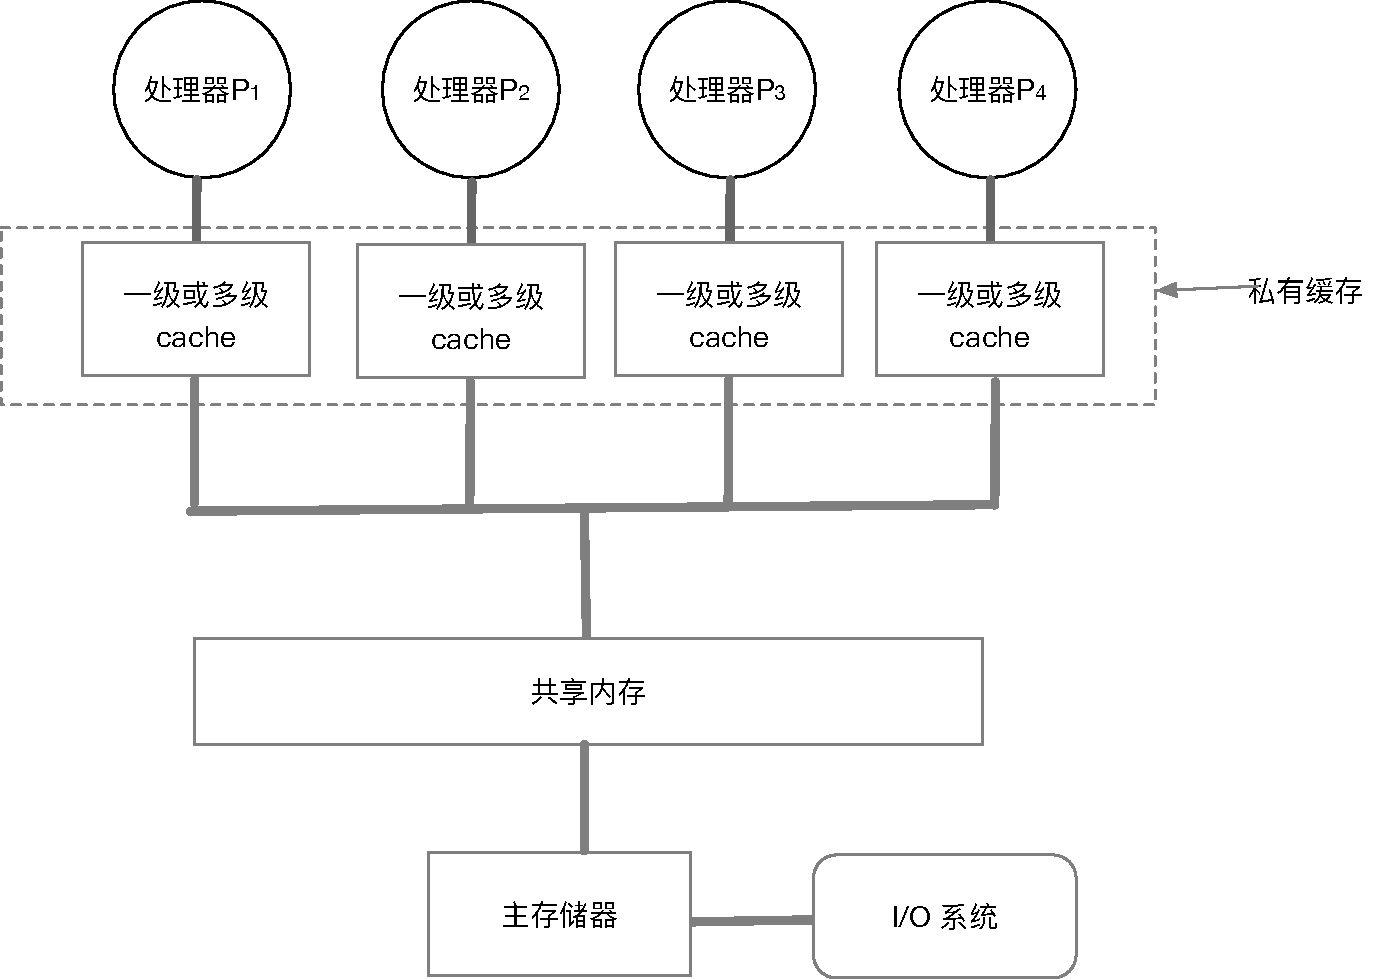
\includegraphics[width=0.65\textwidth]{uma}
\caption{SMP架构多处理器的基本结构示意图}
\label{fig:uma}
\end{figure}


\begin{itemize}
	\item \textbf{对称多处理器(Symmetric (shared-memory) Multiprocessors,简称SMPs)},又称为集中式共享内存多处理器。
	这种结构的处理器特点是具有少量的处理器,通常为8个或者更少。对于具有如此小的处理器数量的多处理器,所有处理器可以共享一个单一的集中存储器,所有处理器都有相同的访问权限,“对称”因此得名。在每一块多核芯片上,核心之间的内存都采用共享的方式。当前连接的多核芯片的数量大于1时,会为每一块芯片分配单独的内存,此时的内存是分布式的。SMP体系结构的处理器通常也称\textbf{统一的内存访问(Uniform Memory Access,简称UMA)多处理器},这是因为所有的处理器都具有相同的内存延迟。图~\ref{fig:uma}所示为SMP体系结构的多处理器结构图。处理器的缓存子系统共享相同的物理内存,通常情况下具有一级共享内存,每个处理器内的核心具有一级或多级的私有缓存。该架构的重要属性是,所有的处理器具有相同的内存访问时间跟延迟。所有的处理器都必须通过一条总线实现同步与内存访问,因此,统一内存访问架构的多处理器系统的最大性能瓶颈是内存。当系统的处理器个数大于32时,因为总线争用将十分激烈,严重影响多核系统性能使用单总线连接处理器和内存模块的方式不可取。
	\item 当系统内的处理器数量较多时,使用SMP架构会对系统性能造成影响,因此处理器数量较多的系统通常采用\textbf{分布式共享内存(Distributed Shared Memory,简称DSM)}架构,DSM是与SMP相对的一种体系结构,这种结构下的多处理器共享逻辑地址空间,但是物理内存是分布式的。图~\ref{fig:dsm}所示为DSM体系结构多处理器的结构简图。为了支持更大的处理器数量,系统的内存必须是分布式的。否则,内存系统无法在保持内存访问延迟较低的前提下满足大量处理器的内存带宽需求。随着处理器性能的快速增加以及随之增长的内存带宽的需求,分布式内存要求的多处理器的规模将持续缩小。将内存分布在不同的结点上不仅增加了内存带宽,同时也满足了处理器访问内存低延迟的要求。由于访问时间取决于数据在本地内存结点还是远程内存结点上,因此,DSM多处理器通常也被称为\textbf{非一致的内存访问(Non Uniform Memory Access,简称NUMA)}多处理器。DSM的主要缺点是处理器之间的数据传输更加复杂,若要充分利用分布式存储器提供的更高的内存带宽需要花费更多的精力进行软件设计。
\end{itemize}

在SMP和DSM两种体系结构的多处理器中,线程之间的通信都是通过共享地址空间进行的,这意味着只要处理器具有必要的访问权限,任何处理器都可以在任何内存位置上进行内存引用。
与SMP和DSM相关的术语\textbf{共享内存}是指地址空间是共享的。

\begin{figure}
\centering
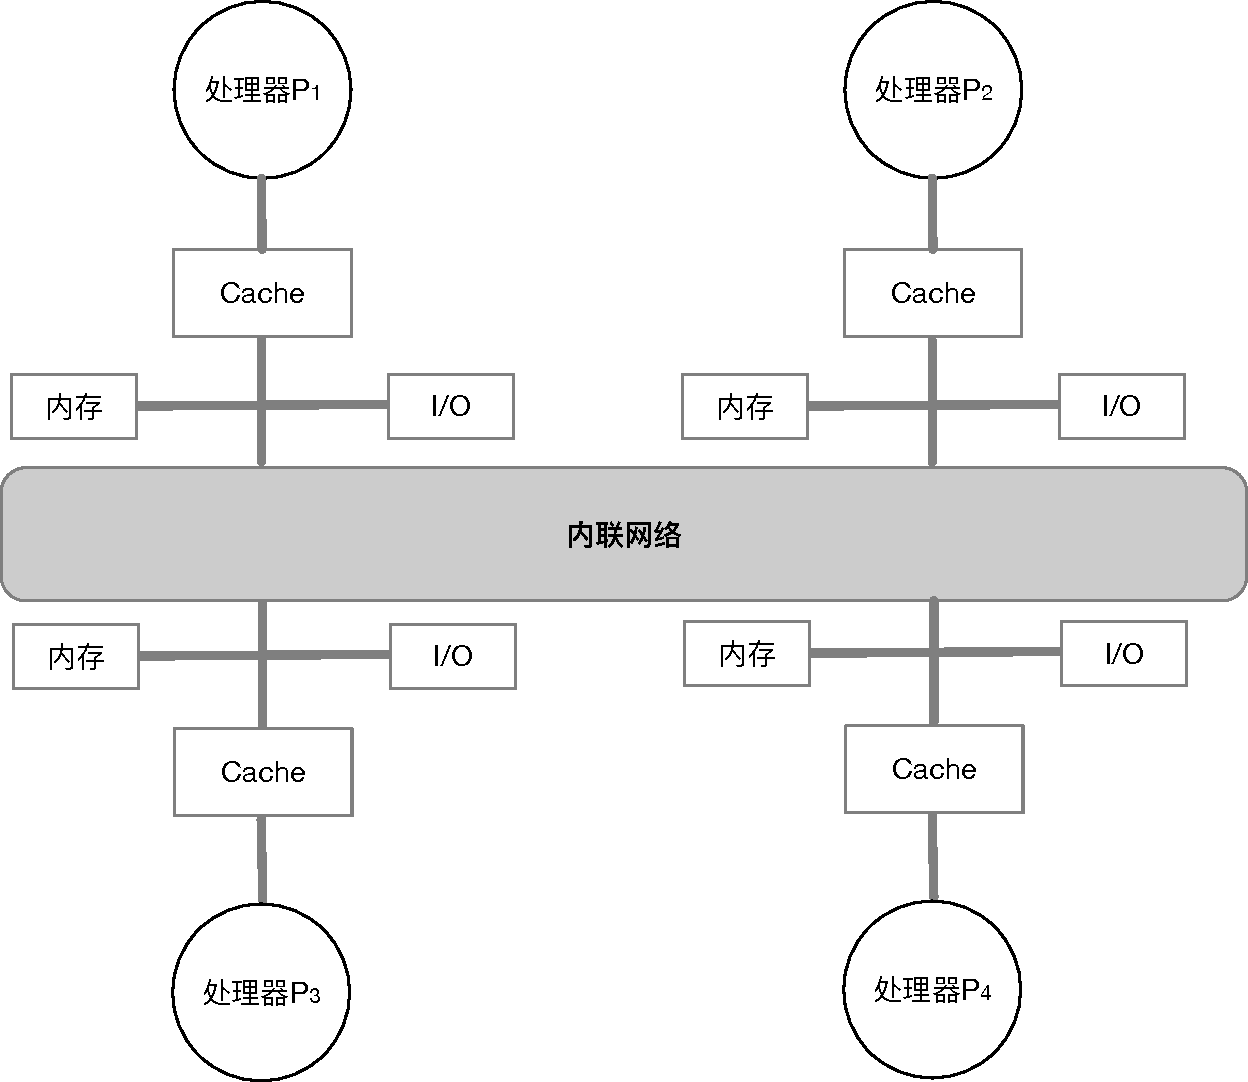
\includegraphics[width=0.65\textwidth]{dsm}
\caption{DSM架构多处理器结构示意图}
\label{fig:dsm}
\end{figure}


如果每个处理器上都具有一个调度器使系统上的多个CPU可以并行的执行任务。
这样的处理器系统被称为对称多处理(symmetric multiprocessing,简称SMP)系统。

负载均衡是多处理器系统的一个显著特点。
如果内核上的进程分布不均衡,即便是系统中的处理器数量再多,对于性能的提升也是微乎其微的。
对称多处理器系统实现负载均衡有两种途径:
第一种方法是将“准备就绪”的进程插入到一个可以共用进程队列中,每个处理器上的调度器都能访问这个进程队列。
当某个处理器中的调度器被激活时,它将从“准备就绪”的进程队列中选取一个进程进入处理器进行运算。
对称多处理系统通过使用共用的“准备就绪”的进程队列实现负载自动均衡。
当某个处理器为空闲状态时,它的调度器会从队列中选取一个进程,并开始在该处理器上运行。
这种方法能够实现处理器负载的自动均衡,但是共用的进程队列实现较为困难。

因此,为SMP设计的现代操作系统通常为每个处理器分配一个进程队列。
这种操作系统使用显示的负载均衡机制,通过这个机制,过载的处理器上的等待列表中的进程会被移动到另外的负载较少的处理器的进程队列中。
例如,SMP Linux系统每间隔200毫秒就激活一次负载均衡机制\cite{bolla2008effective}。
这种方法也存在一个问题,当每个核心都具有私有缓存时,将进程迁移到不同的处理器上的代价高昂。
因此一些操作系统(如Linux)提供一个系统调用来指定与处理器绑定的进程,这与处理器负载无关。

\textbf{多核处理器和多处理器的区别与联系}:多核处理器是指一个CPU内包含若干个计算单元;而多处理器是指在计算机内存在多个相同的CPU。
以双核处理器为例,双核心的设置类似于在同一台计算机上安装两个独立的处理器,但是由于两个核心实际上位于同一块芯片上,它们之间的信息交换的速度要快于同一台计算机上的两个独立的处理器之间的通信速度。
多处理器的CPU可以是由多个普通的只具有一个核心的CPU构成,也可以是由多个多核CPU构成。

在本文的研究中,所用的三个实验平台都是基于NUMA架构的多处理器系统。


% \subsection{设计并发哈希表面临的挑战}
% 设计并发数据结构的挑战主要源自并发性:线程在不同的处理器上并发的执行,并受到来自操作系统调度决策,页错误,中断等因素的影响。
% 因此为了保证不同线程的执行步骤可以任意交错,必须将各个线程的计算步骤看成是完全异步的。
% 这个要求显著增加了正确的设计并发数据结构的复杂度。

% 为多处理器系统设计并发数据结构同样在性能和可扩展性上也面临许多挑战。
% 在当今的主流多处理器架构上,处理器和内存的分布方式,数据在内存中的分布方式,多处理器体系结构的各个环节上的通信负载都对性能产生重要影响。
% 除此之外,正确性和性能问题彼此紧密相关:寻求提高性能的算法优化往往使设计和验证并发数据结构的正确性变得更加困难。

% 下面将以简单的支持FAI操作的共享计数器的实现阐述多处理器的特征如何影响并发数据结构的设计。
% 假设对于共享计数器,有这样一个需求:在进行自增操作之前需要返回当前的计数值。
% 如果允许多个线程同时调用FAI操作,则上述的共享计数器可能出现不正确的行为。
% 大部分编译器在进行编译时,会按照如下顺序将源代码转化为机器指令:1)将$x$载入寄存器内;2)对应的寄存器加1;3)将寄存器内的值存入$x$。
% 假设计数器的初始化值为0,来自不同处理器的两个线程同时调用了FAI操作,则存在两次操作都读取到$x$的值为0的风险,因此都将1存入$x$并且返回0。
% 这显然是不正确的:其中一个操作的返回值应该为1。

% 引发上述问题的原因在于执行FAI操作的两个线程的计算步骤的相互干扰。
% 一般的避免这种相互干扰通常使用\textbf{互斥锁}。
% 锁是一种在任何时刻都处于无主状态或者被单个线程独占的构造。
% 如果线程$t_1$需要获取被线程$t_2$占有的锁,则$t_1$必须等到$t_2$释放该锁。

% \begin{figure}
% \centering
% 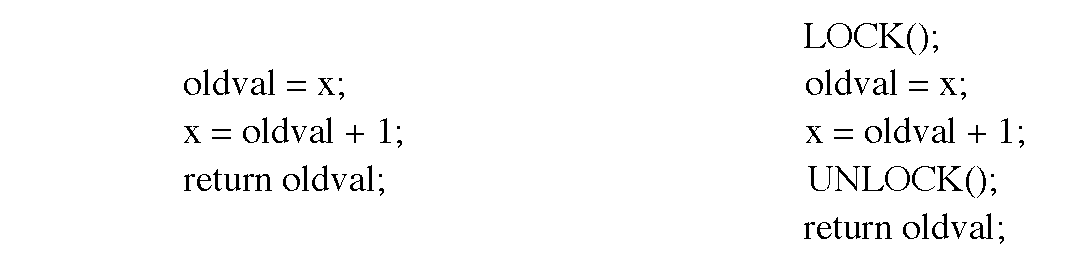
\includegraphics[width=0.65\textwidth]{FAI}
% \caption{串行和基于锁的FAI操作}
% \label{fig:FAI_fragment}
% \end{figure}
% 可以通过图~\ref{fig:FAI_fragment}右侧代码所示的锁来确保多个线程以正确的顺序调用FAI操作。
% 通过这种方法,可以有效避免相互干扰引起的程序不当行为。
% 使用锁方法可以很容易实现正确的共享计数器,但是这种简单性是建立在引入一系列与性能和软件工程相关的问题的基础之上的。

% \subsection{并发哈希表的应用}
% \subsection{}

\section{课题研究背景及意义}

并发哈希表(CHT)是一种允许在同一时刻有多个读者或写者访问共享对象的哈希表。
其提供与串行哈希表一样的访问接口,但是CHT能够更有效的发挥多核处理器的性能。
对于所有并发数据结构而言,断言并发访问是一项必要工作。
在并发编程模型里基于锁和无锁是两种常用的同步控制方式,用于确保多个线程有序的对内存进行访问。
为了保证线程安全性,基于锁的并发哈希表对临界区进行加锁操作。锁的实现有粗、细两种不同的粒度。
粗粒度锁在实现上相对简单,但是采用粗粒度锁往往临界区特别长,阻碍对计算机资源的高效利用。
使用细粒度锁的好处是允许多个线程对数据的不同区段进行并发的读/写。
锁的粒度越细,越有利于提升整体性能,但是同时在实现和正确性验证上也需要耗费更多的精力。
另一种相对的并发编程范式是无锁。无锁化编程是用计算机原语来代替显示锁的一种并发编程范式。
此外还有使用非阻塞方法实现的并发哈希表\cite{}([9~10])。

\subsection{并发哈希表的性能评估}
 
对于并发哈希算法的评估指标主要包括:吞吐量;哈希表的线程扩展性;操作的延迟;内存使用情况;哈希表的空间利用率等方面。
吞吐量是指在单位时间内哈希表执行插入、删除、查询操作的总量,单位为Mops/s或者ops/ms。
线程扩展性是用来衡量运行在多处理器机器上的应用的效率的重要指标。
应用程序的线程扩展性是指随着程序启用的物理线程的数量的增加,应用的吞吐量保持不减的能力。
理想情况下程序的性能应该与物理线程的数量呈线性关系。
延迟是指平均每执行一次哈希表操作需要耗费的CPU时钟周期数。
内存使用情况是指处理同等规模的数据下,消耗的内存。
哈希表的空间利用率是指哈希表在不进行扩容操作的前提下性能达到饱和时,哈希表内实体的数量与哈希表存储能力的比值,在有些文献中哈希表的空间利用率也被称作负载因子(load factor)。

在现有的相关研究成果中\cite{clht,cuckoo,hopscotch,metreveli2012cphash,nonblocking,nonblocking},对哈希表进行评估时所使用的哈希表的设计方法、优化方案、内存分配与管理、测试环境、测试数据、性能评估指标等方面都存在出入。
设计方法上的差异体现在哈希函数的选取;采用什么样的冲突处理方法处理发生冲突的数据;采用哪种同步方法实现多个线程的并发访问。

Y.Liu等人设计了一种可动态调整哈希表大小的无阻塞并发哈希表\cite{nonblocking}。
他们的算法是基于Java的,都使用java.util.concurrent包进行优化。
他们对并发哈希表进行评估时选取使用了相同的冲突处理技术和类似同步方法的SplitOrder哈希表\cite{shalev2006split}的吞吐量曲线和线程扩展性曲线作为基准线,测试在两种不同的多核处理器架构上(X86和SPRAC)展开。
因为这类哈希表支持动态调整哈希表的大小,所以对于哈希表的空间利用率的评估意义不大。

Z.Metreveli等人设计了一种缓存分区哈希表——CPHash\cite{metreveli2012cphash},CPHash将查找/插入请求通过消息传递机制传输到指定的缓存分区内(分区的大小设置为缓存行的大小)。这种设计的目的有两个:一是使用消息传递机制替代传统的锁;二是采用批处理的方式避免过于频繁的缓存行切换。
所以对CPHash的性能评估侧重其与基于锁的同类哈希表的比较,突出消息传递机制取代锁方法的重要意义。

X.Li等人在传统的Cuckoo哈希表的基础上实现了支持多读多写的并发Cuckoo哈希表\cite{cuckoo}。
由于其独特的组相连设计,它的空间利用率是现有的并发哈希表中最好的之一。
Cuckoo哈希表对锁方法、内存消耗、Cuckoo查找路径都进行了优化,所以对于它的评估主要集中在吞吐量、内存消耗、哈希表的空间利用率等方面。

T.David等人对并发数据结构的评估方法相对来说是目前现有工作中最为全面的\cite{clht}。
他们通过对现有的一些并发数据结果的评估,总结了4条"异步并发(ASCY)"并发编程范式。
遵循这4条ASCY模式设计了缓存行哈希表(CLHT)。
缓存行哈希表的核心思想是对哈希表内的元素进行操作时尽量减少缓存行切换。
所以,对CLHT的评估重点在哈希表的线程扩展性、操作延迟、吞吐量等方面,没有针对硬件平台的特点进行优化。

从上述几种并发哈希表的评估方法中可以看出,现有的并发哈希表的评估方法都紧密围绕其设计方法展开的,这样的评估方法缺乏客观性:放大了自身方法优于其它方法的点,而选择性的隐藏自身方法中的性能瓶颈与问题。
这对并发哈希表的设计、优化、应用都是不利的。
用户无法直观判断在其应用中选择哪种并发哈希表能够获得更高的性能。

因此,设计一个统一的测试框架,为并发哈希表的评估提供公平的测试环境,排除因硬件特性、线程分配、内存管理、数据分布、数据集的差别等因素的影响,
充分从吞吐量、线程扩展性、内存消耗、同步方法、延迟、实现的难易程度等方面予以考察,确定设计和使用并发哈希表的最佳实践意义重大。

\subsection{并发哈希表的设计}
设计具有线程扩展性和充分利用处理器多核心优势的并发哈希表是一项富有挑战性的工作\cite{}。
即使是在特定的平台上实现一个达到预期性能要求的具有可扩展性的并发哈希表也是具有相当难度的课题。
在某种体系结构上所采用的优化方法可能会在其他的体系结构上失去作用\cite{}。
比如,针对NUMA架构的多处理器使用的优化方法对与SMP架构的系统就没有任何意义\cite{}。
针对某种硬件特性使用的优化方案在不支持这种硬件指令的系统上甚至都无法实现正常编译。
比如使用RTM优化的并发哈希表在不支持RTM的机器上无法编译\cite{}。
再者,如果某个并发哈希表是针对特定类型的工作集而进行的优化,那么工作集轻微的变化将造成性能的不稳定或者极速下降。
如使用RCU机制设计的并发哈希表,总所周知,RCU机制适合用于处理读占绝大多数的数据集,但是对于数据集中包含有更新操作的场景,使用这种即是实现的并发哈希表的性能甚至无法达到单个处理器系统的同类串行的哈希表\cite{urcu}。

本文的目标之一是要探究是否可以确定并发哈希表的特性。
确定这些特性有助于实现并发哈希表的\textit{可移植的扩展性},即在不同的平台、工作负载和性能指标上都具有扩展性。
乍一看,这个目标可能看起来很模糊,因为它提出了一个根本性的问题:在综合考虑数据结构、体系结构、性能指标和工作负载的前提条件下,我们可以期望获得具有哪种程度可扩展性?

实际上,根据特定的硬件特征和工作负载可以推算出所设计的并发哈希表的可扩展性的上界。
研究表明,对于现代的多核处理器而言,由对共享数据的存储操作引发的一致性流量是抑制并发软件可扩展性的最大障碍。
然而,受并发数据结构固有语义的限制,并发数据结构中不得不存在一定比例的存储操作,这些存储操作是无法省略或者被其他操作替换的;
通常在这些数据结构的串行版本中(即不支持多个进程共享的同种数据结构)也有相同的存储操作。
假设将这样的串行数据结构部署到多核系统上并且由多线程共享该数据结构,显然会得到错误的(如非线性化\cite{herlihy1990linearizability})执行结果。
然而,这种异步执行的程序的性能指明了如何对这些数据结构进行设计确保实现正确的同步。

在追求高性能并发数据结构的过程中,同步控制的软/硬件支持同样是一大挑战。
在多核多处理器平台上,数据的一致性由硬件缓存一致性协议保障。
缓存一致性协议维护读、写和原子指令(比如CAS和FAI)之间的状态转换。
比如,一致性协议可以选择不同的写和无效转换,如读后写,写后写,读无效,写无效。
状态转换影响缓存间的流量,从而影响实际工作的可用缓存带宽。
现代计算机处理器通常使用MESI(Modified-Exclusive-Shared-Invalid)缓存一致性协议和它的其他变体,如AMD的Opteron处理器使用从MESI 中演化出的MOESI协议,O(Owned)是MESI中S和M的一个合体,表示缓存行被修改,和内存中的数据不一致,不过其它的核可以有这份数据的拷贝,状态为S;
Intel酷睿i7处理器使用从MESI中演化出的MESIF协议,F(Forward)从Share中演化而来,缓存行如果处于Forward状态,它可以把数据直接传给其它核心的Cache,而Share则不支持该功能。

硬件事务内存是基于缓存一致性协议的用于进行同步控制的指令集扩展。
当前的技术比较成熟,应用较为广泛的硬件事务内存主要是Intel的事务同步扩展指令集(TSX)\cite{},包括硬件锁省音(HLE)和限制性事务内存(RTM)两套不同的指令集扩展。
使用Intel TSX构造并发哈希表存在的最大问题就是如何避免lemming效应对事务内存性能的抑制作用。

而软件上的同步机制按照发生数据冲突时线程的行为分为阻塞、非阻塞两大类。
阻塞是指在运行多线程(多进程)程序时,当某个线程(进程)在执行临界区时出现延迟,从而导致其他等待进入该临界区的线程(进程)全部延迟的情形;
非阻塞是相对阻塞而言的概念。
具体细分下来阻塞技术又包括锁方法、屏障技术,非阻塞技术又包括无锁(lock-free)、无等待(wait-free)等方法。
读-复制更新(Read-copy Update,RCU)是一套无锁化编程机制,由于其安全性高、性能稳定等原因被广泛用于Linux操作系统内核中\cite{mckenney2003kernel,mckenney2004scaling,mckenney2013rcu}。

\subsection{哈希表与布隆过滤器}

在数据库、缓存、路由器和存储系统中,经常需要进行\textit{近似集合成员关系查询}以确定某个元素是否属于某个集合的成员。
布隆过滤器是一种空间效率很高的随机数据结构,它利用位数组很简洁的表示一个结合,并能判断一个元素是否属于这个集合。
数据据量较小的情况下,使用哈希表、集合、位数组等方法都能完美解决问题。
但是在大数据的背景下对拥有巨量的元素信息的应用场景而言,如果按照常规的方法存储元素的完整信息,所需的存储空间将给存储系统造成巨大的负担。
这种情况下布隆过滤器有了用武之地。
布隆过滤器具有极高的空间利用率,用来解决海量数据的索引问题最合适。
它核心思想是利用多个不同的哈希函数来解决集合元素查询时产生的冲突问题。
布隆过滤器被广泛应用于概率路由表中减少内存空间的需求\cite{yu2009buffalo};
用于加速IP地址的最长前缀匹配\cite{dharmapurikar2003longest};
用于提升网络状态管理和监控\cite{bonomi2006beyond,song2005fast};
用于网络数据包组播转发信息的编码\cite{jokela2009lipsin},以及其他的网络应用\cite{broder2004network}。

然而,布隆过滤器存在两个缺陷:一是由于元素信息使用位数组保存,所以不能支持元素的删除操作;二是因为哈希函数存在碰撞导致布隆过滤器在进行元素查询时存在一定的误报率。
虽然在后续的研究成果当中,出现了支持元素删除操作的布隆过滤器的升级版本,比如Counting布隆过滤器\cite{fan2000summary}、d-left counting布隆过滤器\cite{bonomi2006improved}以及quotient过滤器\cite{bender2012don}。
但是这些过滤器要么是牺牲了空间效率,要么是牺牲了性能。
为了保持相同的误判率,counting布隆过滤器需要使用3-4倍的存储空间用于表示一个元素,d-left counting布隆过滤器则需要1.5倍的存储空间,而quotient过滤器获得同等的空间效率它的查询性能要大打折扣。

此外,在当前多核处理器越来越受重视的背景下,没有一款支持多线程并发的布隆过滤器。
考虑到布隆过滤器的核心功能是通过哈希函数计算元素存储位置的索引值,这与构建并发哈希表存在相通之处,可以重用哈希表的同步方法、哈希方法、哈希表结构。
另外,Cuckoo哈希方法能够确保哈希表在空间利用率达到95\%左右时,仍然能够保证具有较好的性能。
所以,设计基于Cuckoo哈希方法的Cuckoo过滤器是能解决当前的布隆过滤器方法中需要耗费大量存储空间实现删除操作或者需要牺牲查询性能换取对删除操作的支持的问题。此外,还能弥补对并发布隆过滤器的研究领域的空缺。

综上所述,研究并发哈希表在多核系统上的软/硬件同步方法,对于并发哈希表的优化与设计具有重要的理论意义。
研究新的硬件同步机制对于构建并发数据结构以及提高现有并发数据结构的性能、简化并发数据结构的设计、实现新的并发数据结构具有重要的实用价值。


\section{本文主要工作}
本文主要着眼主流多核处理器架构上的并发哈希表的优化、设计与应用研究。

首先,设计了一个用于测试基于多核系统架构的并发哈希表的测试框架——CHTBench,CHTBench为并发哈希表提供公平测试环境和统一测试接口。使用CHTBench进行测试可以兼容不同的硬件平台、工作集、并发模型以及编译选项配置,在进行性能评估的比较时,排除上述因素的干扰,确保测试结果的公平性。
对并发哈希表的线程扩展性、吞吐量、运行时延迟、工作集的大小与读写比例、多核系统的内存分层结构、底层同步原语、内存消耗以及实现的复杂度等8个维度进行比较分析,在必要时还对存在关联的指标进行深入分析。实验平台涵盖了主流的SMP架构和DSM架构多核处理器以及众核架构(MIC)多处理器系统。
其中,本文中将并发哈希表这种数据结构移植到Xeon Phi平台上进行同步性能评估的工作是已知的最先将并发哈希表的研究延伸到MIC架构上。
此外,根据每一项评估指标的实验结果提出了与该指标相关的性能陷阱和优化误区,并提出了在设计并发哈希表时存在相互矛盾的性能指标的情况下,如何进行折衷与优化,以对并发哈希表的优化、设计提供指导意见。

第二,根据对并发哈希表的评估结果进行分析得到的最佳设计实践原则,设计了基于硬件事务内存的缓存行哈希表。
原始的缓存行哈希表的并发操作使用的是细粒度锁实现的,使用链式反应法解决哈希冲突问题,具有极高的吞吐量,极佳的线程扩展性和极低的操作延迟。
考虑到细粒度锁方法实现的复杂性和难以保障正确性(比如经典的ABA问题)等缺陷,本文使用硬件事务内存实现并发缓存行哈希表。
使用硬件事务内存实现的全局锁获得了比使用常规的细粒度锁更高的吞吐量。
此外,为了降低Lemming效应对Intel TSX性能的副作用,提出了两种软件辅助方法:软件辅助的锁省略方法(SLR)和软件辅助的冲突管理方法(SCM)。

最后,设计了支持并发操作的Cuckoo过滤器。
布隆过滤器是一种判断元素是否属于集合的数据结构,它允许一定的假阳性率换取存储空间的极大节省,是哈希表的具体应用,但是当前的布隆过滤器有两个缺陷:不支持并发,不支持删除操作。
本文使用基于HTM的读写锁实现了支持多线程并发的Cuckoo过滤器,并使用不完整Cuckoo哈希方法实现了删除操作。
通过理论推算表明布隆过滤器的空间效率要优于Cuckoo过滤器,但是通过我们的实验评估结果表明,这种差距产生的影响很微弱。
相比于其他支持删除操作的布隆过滤器的变体而言,Cuckoo过滤器的空间效率的优势十分突出。

% 本文各项工作中多核体系结构是研究的基础,基于硬件事务内存的并发哈希表的设计是研究的出发点,并发哈希表的应用是研究的最终目的。

\section{本文组织结构}
本文分五个章节展开,各章大体内容安排如下:

\textbf{第一章}概述多核系统架构的基本概念及多核处理器在当前的经济生活与技术发展中的重要意义,以此为基础综述NUMA架构多处理器的内存管理、基于多核架构的并发哈希表的研究的现状与缺陷、硬件事务内存对基于多核架构的并发数据结构的作用以及布隆过滤器的原理与缺陷等问题。
指出当前基于多核系统架构的并发哈希表的优化、设计与应用中存在的问题及其研究的意义。
最后归纳本文的主要工作以及论文组织结构。

\textbf{第二章}介绍与本文密切相关的并发哈希表的概念、设计方法与相关研究成果。
介绍用于实现并发数据结构的同步方法,包括锁算法、屏障方法、非阻塞方法和硬件事务内存。
然后对NUMA架构下的内存管理研究成果进行了概述。
最后,对哈希表的一个重要应用——布隆过滤器的相关研究成果进行介绍。

\textbf{第三章}选取5种基于不同设计方法的具有代表性的并发哈希表进行评估。首先着重介绍了用于在多核系统上对并发哈希表进行测试的测试框架CHTBench,然后对所选的5种并发哈希表的设计方法、数据结构特点以及同步原理进行了描述,随后根据这5种并发哈希表在CHTBench上的运行结果总结了8条设计、优化和应用并发哈希表的最佳实践原则,最后是对这一章的小结。

\textbf{第四章}根据前一章总结的8条最佳实践原则以及硬件事务内存在实现并发数据结构上的优势,设计了基于硬件事务内存的并发缓存行哈希表。
然后介绍了用于克服Lemming效应对Intel TSX的软件辅助方法——软件辅助的锁省略技术和软件辅助的冲突管理技术。
接下来是对基于硬件事务内存的缓存行哈希表的评估,评估同样是在CHTBench框架上展开。

\textbf{第五章}介绍支持删除操作的并发Cuckoo过滤器。
首先对传统的布隆过滤器实现最优误判率、空间利用率的参数进行推算;然后对基于不完整键Cuckoo哈希方法的进行介绍,并对达到最优空间效率和误判率的相关参数进行了推算;接下来并发Cuckoo过滤器的插入、查询和删除操作的实现进行了介绍,再是对Cuckoo过滤器的评估结果以及根据评估结果进行的优化。
最后对这章内容进行总结。


%  \chapter{并发哈希表的相关研究}

% 引子

\section{哈希表概述}

\subsection{相关概念}

哈希表、树、链表等都属于搜索数据结构。
搜索数据结构由元素集合以及访问和操作这些元素的接口构成。
如果搜索数据结构能够被多个处理器共享,我们则称该数据结构为\textbf{并发搜索数据结构}(CSDS)。
哈希表(hash table),又名散列表,是一种应用广泛的搜索数据结构,它通过键值对(key-value)实现对关联数据的高效存取。
键值对之间的映射关系称为\textbf{哈希函数}。
一般的哈希表都提供了\textit{add(),remove()}和\textit{find()}三种操作的接口。
哈希表的操作分为\textbf{读}操作和\textbf{写}操作,其中读操作指哈希表的查询操作,写操作包括在哈希表中插入和删除元素。
哈希表和树型数据结构相比的最大的优势是哈希表的查询复杂度可以到常数级。
存放值的存储空间称为\textbf{哈希桶}(bucket)或者\textbf{哈希槽}(slot)。
哈希表中存放的元素的数量与哈希桶数量的比值称为\textbf{负载因子}(load factor)。
哈希表使用哈希函数计算得到一个索引值,该索引值表明键对应的值在桶数组中的位置。
关于哈希函数,有一个最理想的原则:将每一个key映射到单独的哈希桶内。
但是,当数据集规模很大时,能够完美的践行上述原则的哈希函数并不存在。
因此在实际的映射过程中往往会出现多个key对应相同的索引值,这时称为发生了\textbf{碰撞}(collision)。
既然碰撞无法避免,那么我们能做的就是在设计哈希表的时候尽量的选择好的哈希函数。
一个好哈希函数的基本需求是输出的哈希值比较均匀。
这样可以使发生碰撞的概率最小化,同时使得各个bucket中碰撞的条目比较平均。
有国外的研究人员对已有的哈希函数做过比较~\cite{Josh2012},结论是MurmurHash3~\cite{Murmurhash}~和CityHash~\cite{cityhash}~是迄今为止最出色的哈希函数。

\subsection{哈希函数}
哈希函数是将任意大小的数据转换成特定大小的数据的函数,转换后的数据称为哈希值或哈希编码。
哈希函数是实现哈希表和布隆过滤器的基础。
根据其应用场景可以划分成加密和非加密两类。
非加密的哈希函数通过数学运算将字符串转化成整型数输出。
哈希函数的一个重要特点是它的输出能够在可能的输出域内尽量的保证均匀分布,尤其是当具有比较相近的输入时,这种特性尤为可贵。
与加密哈希函数所不同的是,非加密哈希函数无法承担阻止攻击者利用碰撞进行攻击的任务。
非加密哈希函数的运算速度要比加密哈希函数快。
哈希表通常采用非加密哈希函数建立元素与哈希表的对应关系。

Bob Jenkins长期从事哈希函数的研究,他在1997年对哈希函数的研究中提出了被后来研究人员称为Jenkins的哈希函数\cite{jenkins1997hash},在接下来的研究中,他对其研究成果进行了扩展,提出了名为lookup2和lookup3的哈希函数\cite{jenkins2006function}。lookup3哈希函数被有关学者认为是第一款“现代的”哈希函数。
2008年,Austin Appleby发布了名为MurmurHash的哈希函数\cite{Murmurhash}。
最新的Murmurhash具有两倍于lookup3的性能。由于其卓越的运算速度和统计特性,MurmurHash得到广泛应用。
2011年,发布了两款高性能的哈希函数:一款是Google发布的CityHash\cite{cityhash};另一款是由Jenkins提出的SpookyHash\cite{jenkins2012spookyhash}。这两款哈希函数都是基于MurmurHash,其性能的提升在很大程度上得益于更高的指令集并行。
这两款哈希函数都有两倍于MurmurHash的处理速度,CityHash的速度源于SSE 4.2中的CRC32指令。
SpookyHash产生128的输出结果,而CityHash的输出结果更为灵活,可生成64位、128位和256位的哈希值。

\subsection{哈希冲突处理}

处理碰撞的方法大致可以分为两类:一类是\textbf{开放寻址法}(open-addressing);一类是\textbf{开链法}(separate chaining)。

开放寻址法,所有元素都存放在哈希桶数组内,当需要在哈希表中插入新元素时,将对哈希桶进行扫描,从被直接映射到的哈希桶开始,按照某种探测序列进行扫描,知道找到空闲的哈希桶为止。
当需要查找某个元素时,需要以同样的探测序列进行查找,直到找到所需的元素,或者最终发现元素不在表中为止。
常用于开放寻址法的探测序列有线性探测、二次探测、双重哈希以及Cuckoo哈希。

\textbf{线性探测}。
在线性探测中,进行探测的初始位置由$h(k)$确定,地址增量为$i$,从当前位置开始,若为空,则插入元素,若非空,则探测距离当前位置$i$个单位的位置继续,直到找到空闲的位置或者便利完整个哈希表为止。
为了确保能够遍历到整个哈希表,$i$通常是哈希表容量$m$的相对质数。
利用线性探测计算key的位置的公式如式~\ref{equ:linear_prob}所示:
\begin{equation}
	h(k,i) = (h(k)+i) ~{mod}~m
\label{equ:linear_prob}
\end{equation}
当地址增量$i$等于1时,探测的位置是连续的。
线性探测的性能取决于查找key的位置时进行的探测次数,而探测次数又取决于哈希表的负载因子。
哈希表的负载因子越高,查找一个key的位置时所需的探测次数就越多。
Knuth的论证表明\cite{knuth1998art},使用线性探测法完成一次key的位置探测所需的平均探测次数约为$1/2(1+\frac{1}{1-\alpha})$。


\textbf{二次探测}与线性探测的相关性很高。
二次探测计算key的位置的公式如式~\ref{equ:quad_prob}所示:
\begin{equation}
h(k,i) = (h(k)+c_1 i+c_2i^2)~{mod}~m
\label{equ:quad_prob}
\end{equation}
式中$c_1$和$c_2$均为常数。
Heileman等人的研究表明,当哈希表的大小超过缓存的容量时,使用线性探测的性能要好于使用二次探测\cite{heileman2005caching}。
虽然线性探测通常需要比二次探测执行更多的探测尝试,但是这些尝试具有更高的缓存命中率,从而在整个哈希表的大小超过了缓存容量时表现出更好的整体性能。
另一方面,当哈希表的负载因子较高时,使用二次探测能够获得更好的性能,当然这只是相对而言的,当$\alpha$接近1时,使用二次探测的性能也不理想\cite{}。
同样Knuth对使用二次探测完成一次key的位置的探测所需的平均探测次数进行了估计,约为$1-ln(1-\alpha)-\frac{\alpha}{2}$。

\textbf{双重哈希},顾名思义就是使用两个哈希函数$h_1$和$h_2$计算需要探测的初始索引值。
计算公式如式~\ref{equ:double}所示:
\begin{equation}
h(k,i) = (h_1(k)+i\cdot h_2(k)) ~{mod}~m
\label{equ:double}
\end{equation}
由于$h_2$提供可变的地址增量,所以双重哈希很好的解决了线性探测和二次探测中的“聚集”问题。
此外,多重碰撞的设置产生比线性或二次探测更为均匀的键值分布。
双重哈希方法的性能也会随着哈希表负载因子的增加而下降。
使用双重哈希完成一次查找所需的平均探测次数为$-\frac{1}{\alpha}ln(1-\alpha)$。

\textbf{Cuckoo哈希}
Cuckoo哈希的特性是当在哈希表中插入新的key时,会将原来存储与该位置上的key排挤到其他的位置上去。
一般设置两个哈希函数$h_1(k)$和$h_2(k)$。
当插入新的key时,可以任意的选择在$h_1(k)$和$h_2(k)$位置上进行插入。
如果插入的位置上已经存有了$k_1$,则将$k$覆盖$k_1$,然后将$k_1$存入到$h_1(k)$和$h_2(k)$中空闲的位置。
如果$h_1(k)$和$h_2(k)$中都没有空闲位置,则继续上述过程,直到所有的key都找到了合适的位置或者执行替换的次数达到上限\cite{pagh2004cuckoo,erlingsson2006cool}。
Pagh等人的研究表明,要保持Cuckoo哈希的最优性能,需要确保$\alpha\leq 0.5$\cite{pagh2004cuckoo};Erlingsson等人提出了一种广义的Cuckoo哈希技术\cite{erlingsson2006cool},能够使哈希表的负载因子达到99\%时仍然具有较好的性能;
Ross等人通过应用单指令多数据流(SIMD)指令挖掘并行性并消除探测函数内的分支指令实现了对广义Cuckoo哈希方法的性能优化\cite{ross2007efficient}。

上述的几种常用的开放寻址法中,性能都与哈希表的负载因子相关。
负载因子越高,完成一次查找所需的探测次数就越多,性能也随之受到影响。
实际上,即便是再好的哈希函数,在负载因子大于0.7之后性能会急剧下降。

另一类常用的冲突处理方法称为开链法。
开链法引入额外的数据结构,比如链表,用于解决哈希冲突问题。
每一个哈希桶都是独立的,所有经过哈希之后具有相同索引值的元素都放在同一个哈希桶中,这些元素通过链表进行管理。
所以,使用开链法的哈希表能够存储的元素的个数大于哈希桶的数目,也就是说它的负载因子可以大于1。
对哈希表执行操作的时间等于找到相应的哈希桶的时间加上对列表进行操作的时间。
虽说使用开链法的哈希表的负载因子可以大于1,并不意味着链入同一个哈希桶中的元素的个数可以是无限制的,如果某一个位置冲突过多的话,插入的时间复杂度将退化为O(N),这种退化将引起缓存未命中率的骤然升高\cite{black1998graph}。
因此,每个哈希桶内元素的个数应在3个以内。

两种方法各有优劣,开放寻址在解决当前冲突的情况下可能会导致新的冲突,而开链不会产生这种问题。另一方面开链的局部性较之开放寻址法要差,在程序运行过程中可能引起操作系统的缺页中断,从而导致系统颠簸。

哈希表被广泛实现系统层和应用层软件,被集成到编程语言如Java,Python等,还可以用来实现关联数组,数据库索引,缓存,集合等。
哈希表的高效性使其具有重要的研究价值和应用价值。

\section{基于软件技术的同步方法研究}

在并发哈希的设计中,除了选用的哈希函数、所采用的冲突处理方案以及数据结构上的差异造成性能上的差别之外,另一个重要的因素是选取的同步方案。
并发数据结构的设计中,常用的同步方法大致可以划分成三类:锁方法、内存屏障技术和事务内存。

\subsection{阻塞技术}
\subsubsection{锁方法}
在并发数据结构中锁用于保证多个线程对数据结构的互斥访问,以避免线程间发生“错误的”交错,从而产生预期之外的结果。
设计锁算法的关键问题是当线程$t_1$试图申请线程$t_2$已经占有的锁时,$t_1$要采取的行动。
在单处理器系统上,出现这种情况时唯一明智的处理方式是将处理器让给$t_1$即可。
但是在多处理器系统上,因为锁可能在不长的时间内会被另一个处理器上执行的线程释放,所以使$t_1$反复尝试获取锁有助于提升性能。
这种使线程不断的尝试获取锁的技术称为\textbf{自旋锁(spinlock)}。
在线程执行期间很难预测该线程会持有锁多长时间,所以很难在阻塞技术和自旋锁之间做出选择。
如果操作系统直接支持锁,诸如当前持有锁的线程等信息能够用于做出抉择。

简单的自旋锁重复使用同步原语,如比较和交换(swap-and-change,CAS),以原子方式将锁从无主状态转换到被占有状态。 如果锁的设计不够仔细,自旋锁会引起激烈的锁竞争,从而对性能造成严重影响。
一种简单的降低锁竞争的方法是引入指数退避(exponential backoff)机制\cite{agarwal1989adaptive}。
使用这种方法获取锁失败的线程在进行重试之前会等待一段时间;
失败的次数越多,等待的时间越长,此时线程会及时的“自行分散”,由此降低了线程对锁的争用,同时也减少了由于尝试获取锁失败引起的流量开销。

使用指数退避机制的锁的缺陷是锁可以处于无主状态,而尝试获取该锁的线程都已经执行退避策略,需要等待较长的时间,因此在这段时间内所有的线程都不会前向执行。
解决这个问题方法是使所有申请锁的线程存储在一个队列中,锁被释放后将锁的所有权传递给下一个正在排队的线程。
基于这种方法实现的锁被称为\textbf{队列锁(quenelocks)}。
Anderson\cite{anderson1989performance}和Graunke\cite{graunke1990synchronization}提出了基于阵列的队列锁方法。
之后M.Crummey和T.Scott\cite{mellor1991algorithms}对他们的方法进行改进实现了的基于列表的MCS队列锁,以及由Craig和E.Hagersten等人\cite{craig1993building,magnusson1994queue}提出的CLH队列锁。

使用CLH锁的线程形成一个虚拟的节点链表,每个节点都包含一个$done$标志;某个线程只有当列表中它的前继节点的$done$标志被触发后才进入临界区。
为了获得锁,线程创建一个节点,将它的$done$标志设置为$false$,表示它还没有释放临界区,并且使用同步原语(如CAS)将它自己的节点放在列表的尾部,同时确定其前继节点。
随后,该线程在其前继节点的$done$标志上自旋。
值得一提的是,每个线程的自旋过程发生在不同的内存位置,因此,在基于缓存的体系结构中,当某个线程设置其$done$标志以通知队列中的下一个线程可以进入临界区时,所有其他正在自旋的线程的$done$标志不会被修改,这些线程将继续 在本地缓存行上自旋,而不会产生额外的内存流量。
这在很大程度上减少了争用,提升了扩展性。
但是,如果使用这种锁算法的程序运行在非一致性的NUMA平台上,某些线程不得不在远程内存结点上进行自旋,这样无疑会消耗更多的内存流量。
使用MCS队列锁\cite{mellor1991algorithms}通过将线程自旋的位置限定在该线程自身结点的$done$标志来解决NUMA平台上的问题。

此外,为了迎合特定的数据结构的数据读取特性在后续的演化中出现了一些标准锁方法的变体。
队列锁算法中出现了一种具有“可中止的”特性的版本,它允许正在申请锁的线程放弃等待,比如在实时性要求较高的应用中延迟超过极限值时\cite{scott2002non,scott2001scalable},或者线程需要从死锁中进行恢复时。
M.Scott等人提出了抢占安全锁(preemption-safe locks)\cite{michael1998nonblocking},它通过确保队列中被抢占的线程不会阻止锁被授予另一个正在运行的线程,从而试图减少锁抢占对性能造成的负面影响。

许多数据结构有并发读取的需求,因此,这样的读写锁只允许线程对临界区内的数据进行读取而不能修改,如果当前临界区没有写者线程进行操作,则允许多个读者线程并发访问。
M.Crummey和T.Scott等人提出的读写队列锁算法是基于MCS队列锁并且使用读计数器和指向写者节点的指针实现的\cite{mellor1991scalable}。
Krieger等人\cite{krieger1993fair}提出了一种通过设置队列节点的双链表的队列锁,这种方法的每个节点都有自己的简单“迷你锁”,读者通过获取其相邻节点的迷你锁并重定向双链表的指针来将自己从queuelock列表中移除。

锁在并发数据结构的设计中的重要性不言而喻。
选取锁的标准一是要与应用场景结合;二是要能提供充分的扩展性。
对于哈希表这种读密集型的数据结构

\subsection{屏障技术}

屏障是这样一种机制,所有的提前执行到代码中指定的某些位置的线程悬停,只有当所有线程都到达这个点时才允许它们继续执行。 当访问数据结构或应用程序需要划分成若干个不相互重叠的执行阶段时,就需要使用内存障碍。
例如,并行垃圾收集器的标记和扫描阶段。
此外,在本文中设计的统一的并发哈希表测试框架就用到了内存屏障。
并发哈希表在测试之前需要进行初始化,也就是在哈希表内插入一些元素,让哈希表的密度达到预定的值。
初始化的过程使用多线程共同完成,由于不需要删除元素,所以这个过程在数据量大的测试集中采用多线程会节约初始化时间。
此时如果有现成提前完成了初始化的任务,它会触碰到内存屏障,必须要等待所有参与初始化的线程全部完成之后再往下执行。

实现屏障的一个简单方法是使用初始化一个值为线程总数的计数器:每个线程在到达屏障后递减计数器,然后自旋,等待计数器变为零,然后继续往下执行。
这种直观的实现方式可能引起两个方面的问题:
\begin{itemize}
	\item 当使用相同的pass/stop技术实现了多个串行屏障时,当有线程到达第二个屏障而在第一个屏障内还有一些线程没有完成时,会出现死锁;
	\item 由于所有的线程反复的查询全局变量的状态,导致通信流量大,从而对程序的可扩展性造成影响。
\end{itemize}
针对上述问题,实现了专门的屏障技术,可以让线程在不同的位置自旋\cite{brooks1986butterfly,hensgen1988two,mellor1992fast,tseng2016scalable}。
或者也可以使用Dijkstra和Scholten风格的发散计算树来实现屏障\cite{dijkstra1980termination}。在这种方法中,每个线程都是二叉树中一个节点的所有者。
线程等候它的子节点的到达,然后通知该线程的父节点以表明自己的子节点已到达。一旦所有线程都已到达,树的根节点通过向下发送释放消息释放所有线程。
除了通过软件技术实现的屏障之外,还有通过硬件实现了上述的屏障功能\cite{solihin2015fundamentals}。

\subsection{无阻塞技术}

如前文所述,使用无阻塞编程是为了克服使用锁方法带来的若干问题。
无阻塞技术包含几类条件——无等待\cite{lamport1974new,herlihy1991wait},无锁\cite{herlihy1991wait}和无阻碍\cite{herlihy2003obstruction}。
三类条件由强到弱排列顺序依次为无等待强于无锁,无锁强于无阻碍。
但是这三类条件都强于使用诸如锁之类的阻塞结构。
虽然更强的前向条件是可取的,但是通常情况下实现较弱的保障条件更加容易、效率更高,并且易于设计和正确性验证。
所以,在实际的应用中,研究人员往往通过采取退避策略\cite{agarwal1989adaptive}或使用更复杂的竞争管理技术\cite{herlihy2003software}来补偿较弱的前向条件。

除了少数特别情况,非阻塞算法使用硬件必须提供的原子读-修改-写原语,其中最值得注意的是比较和交换指令(CAS)。
使用无阻塞方法实现的并发数据结构都是使用这些原语的标准接口实现的(在一般情况下,即使是使用了读-修改-写原子原语,临界区也是阻塞的)。
直到本文撰写,所有的非阻塞算法都必须被“原生”地写入底层原语才能达到预期的性能。

无等待算法具有最强的非阻塞前向保证条件,它保证所有CPU在连续处理有效工作时,没有运算会被其他运算所阻塞。
如果每个操作完成所需的执行步骤是有限的,则认为该算法是无等待的算法。
在性能成本不是太高的前提下这个属性对于实时系统具有非常重要的意义。
早在上个世纪九十年代,Herlihy等人就证明了所有的算法都可以实现无等待版本\cite{herlihy1988impossibility},并且已经证明了很多被称为通用结构的串行代码转换。
但是转化后的性能与设计初衷南辕北辙。
有研究人员对实现无等待算法的难度进行了评估。
比如,文献\cite{fich2004inherent}的研究表明使用CAS、LL/SC等原子条件原语很难在不增加内存消耗和损失线性的线程扩展性的前提下实现一般的数据结构的无饥饿算法。

2011年以后,学术界和工业界对无等待算法的研究才开始重视起来。
2011年,Kogan和Petrank提出了一种基于CAS原语的无等待队列\cite{kogan2011wait},这种无等待队列只需要普通的硬件支持即可实现。
这种无锁队列是对 Michael和Scott\cite{michael1996simple}提出的一种被广泛应用于实际的队列的扩展。
2012年Kogan和Petrank\cite{kogan2012methodology}等人又提出了一种提高无等待算法处理速度的方法并且使用这种方法实现的无等待队列的性能比无锁方法实现的相同的队列性能更好。
2014年,Timnat和Petrank\cite{timnat2014practical}提出了一种将无锁数据结构自动转化成无等待数据结构的机制。
至此,无等待实现可以用于多种数据结构中。

无锁算法允许个别线程处于饥饿状态,但能够确保系统吞吐量。
如果所有线程运行了足够长时间后,至少有一个线程能获得前向执行,那么这个算法是无锁的。
所有的无等待算法都是无锁的。
如果程序的某个或某几个线程被挂起,那么无锁算法能够保证剩下的线程能够顺利的执行。

\section{NUMA架构内存管理相关研究}

\subsection{线程与处理器内核的关联}
当前,NUMA系统上主要使用操作系统的调度程序将应用线程分配给处理器内核。 调度程序考虑系统状态和不同的策略目标(比如“平衡内核负载”或“整合内核上的线程或使内核保持为休眠状态”),然后匹配应用线程和相应的物理内核。 特定线程会在其分配的内核上执行一段时间,之后被交换到内核之外进行等待,因为其他线程也需要执行。 如果另一内核可用,调度程序将选择迁移该线程,以确保及时执行并实现其策略目标。

将线程从一个内核迁移到另一内核会导致NUMA共享内存架构出现问题,因为它会断开线程与其本地内存分配之间的关联。也就是说,线程可能启动时在节点$N_1$上分配内存,因为它运行在$N_1$的内核上。但是当该线程后来迁移至$N_2$的内核上时,之前该线程在$N_1$上保存的数据变成了远程数据,内存访问时间大幅增加。

线程与处理器内核关联。 
处理器关联指线程/进程与特定处理器资源实例相关联的持续性(无论其他实例的可用性如何)。 
通过使用系统 API,或修改操作系统数据结构(比如关联掩码),特定内核或内核集可与应用线程相关联。 然后在制定有关线程寿命的决策时,调度程序会关注这种关联方式。 
例如,线程可能配置成仅在处理器$P_1$的0-3号内核上运行。 
调度程序将在内核0-3之间进行选择,不会考虑将线程迁移至其他节点。

执行处理器关联可确保内存分配对有需要的线程保持局部性。 
不过,实行线程与处理器内核之间的关联也存在缺点。 一般来说,如果本可以使用更好的资源管理方式,处理器关联将会限制调度程序的选择,并产生资源争用现象,从而对系统性能造成不利影响。 
除了阻止调度程序将等待线程分配给未利用的内核外,处理器关联的局限性还会对应用本身产生不利影响,因为其他节点上的额外执行时间无法弥补速度较慢的内存访问。

在进行NUMA系统上的并发哈希表的设计时,必须慎重考虑处理器关联方法是否与其数据结构的特点和共享系统环境相适应。 
值得注意的是,除显式关联外,部分系统提供的处理器关联API还支持向调度程序提供优先级“提示”和关联“建议”。 相比于强制执行显示的线程绑定策略,使用此类建议能够确保在通用案例中实现最佳性能,并在高资源竞争环境下避免限制调度选择\cite{majo2017library}。

\subsection{NUMA系统的非对称互连}
\label{sec:}
NUMA架构的多处理器系统的最显著的特点就是它具有非一致的内存访问时间。
因此,线程和内存的分布对NUMA系统的性能起着至关重要的作用。
NUMA系统的这个特性在操作系统领域衍生出了许多的NUMA感知算法。
这些算法要么侧重为线程分配最近的内存节点上的内存空间\cite{brecht1993importance,lachaize2012memprof,dashti2013traffic},或是将内存也分散在系统中以避免内存控制器和互连链路的过载\cite{dashti2013traffic},或是将共享相同数据的线程放置在同一个内存节点上\cite{tam2007thread,tang2013optimizing}以避免内存控制器的争用\cite{bull2002data,blagodurov2010case,tang2013optimizing},或是将可能产生缓存或内存带宽争用的线程分布在不同的内存节点上。

尽管这些上述的研究注意NUMA架构上的线程和数据的分布方式以发挥NUMA架构的性能,但是这些研究似乎都没有考虑到在未来可能会盛行的一个NUMA系统的重要属性:不对称互连。
现代操作系统旨在减少用于线程间和线程到内存通信的跳数。
运行CPU之间的负载平衡时,Linux首先使用同一节点上的CPU,然后是相隔一跳的CPU,最后是相隔两跳或更多跳数距离的CPU。
这些技术假定节点之间的互连是对称的:即对通过直接链路连接的任何节点对而言,链路具有相同的带宽和相同的等待时间。
然而在现代的NUMA系统中情况并非如此。
也就是说,当节点通过不同带宽的链路连接时,不仅要考虑线程和数据是否放置在相同或不同的节点上,而且还要考虑这些节点是如何连接的。
B.Lepers\cite{lepers2015thread}等人通过研究NUMA系统的非对称性对x86系统的影响,发现在同一个节点上的线程和数据分布相同但节点间连接不同的情况下,性能可能会相差2倍以上。
他们对于节点之间的互连有了新的认识,认为在不对称互连的特性下最好的互连方式是在总内存带宽最大的节点之间进行连接,而不是选择具有最小跳数的节点之间进行互连。
基于这个观点,他们实现了基于Linux系统的动态线程和内存分配算法\cite{lepers2015thread}。


\section{事务内存相关研究}
锁在设计并发数据结构中的关键作用是它允许线程对多个内存单元进行原子的修改,因此没有哪一个线程能够读取这些位置上的任何中间值。
事务内存机制是一种允许用户自定义的将访问多个内存单元的代码片段作为一个原子步\cite{moir2004concurrent}。
这种机制对于简化并发数据结构的设计具有重要的理论和实际意义。单纯的从算法实现上而言,编写代码时不再需要考虑哪些内存访问需要持有锁并且有效的防止了死锁问题。

用于实现并发数据结构的事务机制的灵感来源于广泛用于数据库领域的事务的概念。
虽然两者在概念上相通,但是在共享内存单元上支持事务不同于实现存储在磁盘上的数据元素的事务访问。
因此,在这种情况下,可以对于共享内存单元的事务访问的支持可以使用更加轻量级方法实现。

\subsection{实现事务内存的相关技术}
Kung和Robinson等人提出的乐观并发控制(OOC)\cite{kung1981optimistic}是一种用于实现并发数据结构的事务机制。
OOC的基本原理是在事务结束时短暂的持有全局锁。
但是使用这种方法全局锁是一个性能瓶颈,对线程扩展性造成负面影响。
理想情况下,事务性的访问的实现不应该依赖锁,并且在访问不相交的内存单元的事务之间不需要同步。

多处理器上的事务化支持首先是由Herlihy等人\cite{herlihy1993transactional}提出的,同时他们还提出了一种基于硬件的事务内存的方法。
之后,这种基于硬件的事务内存的方法被Rajwar和Goodman等人扩展到包含硬件锁省略技术\cite{rajwar2001speculative,rajwar2002transactional}。
在他们的方法中使用硬件方法将临界区自动转换为一条事务,通过这种方法使两个或多个实际上不相互冲突的临界区可以并行的执行。

事务内存发展到今天,已经有了软、硬件两种实现:基于软件的事务内存(STM)和基于硬件的事务内存(HTM)。
不论是软件事务内存\cite{spear2010lightweight,saha2006mcrt,shavit1997software,linfei2010,wangruibo2007}还是硬件事务内存\cite{yen2007logtm,moore2006logtm,dalessandro2011hybrid,wangzhaoguo2014}都得到了充分的研究与长足的发展。
随着IBM z系列~\cite{Cain2013Robust}和p系列~\cite{Wang2012Evaluation}处理器的出现标志着硬件事务内存从理论研究上升到实际研究,支持事务内存的Intel Haswell处理器~\cite{Intel2015Intel}的问世,标志着硬件事务内存实验研究走向市场化。

Intel的事务同步扩展指令集(TSX)是唯一一款支持硬件事务内存的商用处理器。
目前硬件事务内存还存在一些问题,比如Intel的Lemming效应\cite{Afek2014Software};再比如硬件事务内存不能保证每次事务的执行都能成功提交,为了保证程序能够正确、顺利的执行,需要为程序设置回退路径处理事务不能成功提交的状况,而这个回退路径的实现往往是通过传统的锁方法实现的。
事务内存能够轻易的用于实现并发数据结构,当能够克服上述问题时,使用硬件事务内存将是设计并发数据结构的首选同步机制。

\subsection{基于事务内存的并发数据结构}

随着支持HTM的多核处理器的问世,基于HTM的并发数据结构也得到了深入的研究。
复旦大学的陈海波等实现了一系列基于HTM的并发树型数据结构\cite{wang2014using,wei2015fast,chen2016fast}。
之后,基于他们对于并发树型数据结构的研究发现由于数据冲突引起的事务中止对基于HTM的并发数据结构造成严重影响。
基于这点考虑提出了Eunomia\cite{wang2017eunomia}。
Eunomia是一种集成了若干条用于减轻事务中止的设计模式,主要用于优化搜索树这一类的数据结构。
Z.Wang等人设计了基于HTM的skip list\cite{wang2013opportunities},通过在RTM模拟器和真实的支持RTM的处理器上对比细粒度锁、无锁方法和硬件事务内存等同步方式的比较,总结了若干条提升硬件事务内存性能的规律。
Afek\cite{Afek2014Software}等人设计了两种用于缓解Intel TSX的Lemming效应的软件优化方法,并将他们的方法与传统的CLH、MCS锁以及单纯的使用HTM的性能进行了比较。
本文基于HTM的并发哈希表的设计以及并发Cuckoo过滤器的设计都借鉴了他们提出的软件辅助方法进行优化。

\section{布隆过滤器}

在数据库、缓存、路由器和存储系统中通常需要使用判定一个元素是否存在在某个集合内,这种判断允许一定的误报率。
进行这种成员关系判定布隆过滤器(bloom filter)是使用得最多的一种数据结构\cite{bloom1970space}。
布隆过滤器最初用于拼写检查和数据库检索,随着计算机处理海量数据的压力与日俱增,布隆过滤器的研究再一次焕发新春\cite{xiekun2009}。
布隆过滤器因其高效的内存效率而备受关注。
前Google研究员吴军\cite{吴军2012数学之美}在其《数学之美》一书中指出,使用布隆过滤器的存储效率大约是使用哈希表处理同等规模数据的4到8倍。

1970年B.Bloom\cite{bloom1970space}提出了一种用于处理拼写检查的过滤器,由于其超高的空间效率和处理速度受到广泛关注,后来者为了纪念B.Bloom的突出贡献,将其创造的这种数据结构命名为Bloom过滤器。
布隆过滤器支持对元素的插入和查询操作。
它具有可变的参数误判率,记作$\epsilon$。
对元素的查询返回两种状态:一是“绝对不存在”;二是“可能存在”(这种可能存在的概率为$1-\epsilon$)。
误判率要求越低,用于表示每个元素所需的比特位越多。

为了弥补标准布隆过滤器不支持元素删除的缺陷,Counting布隆过滤器\cite{fan1998summary}对标准的布隆过滤器进行了扩展。
Counting布隆过滤器的原理很简单,就是将原来的比特数组扩展成计数器数组,当插入某元素时,将对应位置上的计数器加1,删除元素时,对应位置上的计数器减1。一般的,为了防止算数溢出计数器的大小为4比特或者4的倍数比特,所以实现Counting布隆过滤器需要至少4倍于标准布隆过滤器的存储开销。

Blocked布隆过滤器\cite{putze2007cache}重点在于优化查询效率,同样不支持删除操作。
这种过滤器是由若干个小型的布隆过滤器构成的,每个布隆过滤器的大小为一个缓存行的大小。
这一点与缓存行哈希表\cite{clht}的处理方式类似。
每进行一次查询操作,最多造成一次缓存未命中的结果,极大的提高了处理速度。
Blocked布隆过滤器的缺陷是由于各个小型布隆过滤器之间的负载不均衡造成误判率相对较高。

$d$-left Counting布隆过滤器\cite{bonomi2006improved}使用\textit{d-left hashing}\cite{mitzenmacher1999asymptotics}将元素转化为指纹信息存储在哈希表中。
删除元素时,找到对应的指纹信息进行删除。
相比于Counting布隆过滤器,它的实现更简洁,而且空间性能也得到了很大提升,空间开销只有Counting布隆过滤器的50\%,处理同等规模的数据,所需的存储空间约为标准布隆过滤器的1.5到2倍。

Quotient过滤器\cite{bender2012don}同样是一种通过哈希表存储指纹信息以实现元素删除的过滤器。
它使用类似于线性探测的方法定位目标指纹信息的位置,这种方法具有更好的空间局部性。
实现这种方法的代价是需要10\%-25\%的额外空间用于对哈希表内的实体进行编码。
此外,编码后的实体到达目标元素所在的位置时需要解码成实体序列,哈希表的密度越高,实体序列越长。
因此,这种过滤器的性能在哈希表的密度高于75\%后急剧下降。

除了上述一些具有代表性的布隆过滤器的设计方法之外,还有一些用于优化特定应用场景的布隆过滤器,如拆分型布隆过滤器\cite{xiaomingzhong2004},基于分档布隆过滤器\cite{xiekun2007},以及将布隆过滤器扩展到多维空间的布隆过滤器\cite{xiekun2008}等。


\section{本章小结}
并发哈希表因其对元素的查找和更新时间为常数级别的特性而被广泛应用于多核架构上的软件系统的开发。
学术界和工业界对于哈希表的研究重点也从单核处理器转移到多核处理器上。
本章的主要目的在于对与本文研究内容相关的问题的研究现状和亟待解决的问题进行归纳,以期为后面章节的研究提供理论依据。
本章首先对哈希表的基本概念进行了简单介绍,并对决定哈希表个性的哈希函数,哈希冲突处理技术进行了介绍;
然后对用于实现并发哈希表的软件同步方法进行简单的描述和比较;其次,介绍了NUMA架构与本文相关的特性——非对称互连和线程绑定;
再次,介绍了事务内存的发展,实现事务内存的软硬件技术并对事务内存在构建并发数据中的相关研究进行了归纳;
最后对与哈希表密切相关的布隆过滤器技术进行了介绍。



%  
\chapter{用于测试并发哈希表性能的框架——CHTBench}

\section{现有的测试方法比较}
\subsection{方法一}
方法描述:

优缺点:

\subsection{方法二}
方法描述:

优缺点:

\subsection{方法三}
方法描述:

优缺点:

\section{评估的指标选取}

\section{统一的跨平台并发哈希表测试框架的设计}
\label{sec:design_framework}

前文在进行并发哈希表介绍时提到,文献中提出的并发哈希表通常在设计(采用什么样的同步编程模型,基于锁还是无锁),实现(采用什么样的硬件优化方案)以及评估方法(总和的测试集合与测试方法)上都千差万别。
这些差异使得用户在横向上很难直观的进行比较,也很难判断究竟哪种因素限制了并发哈希表的性能。
在这部分内容里,将提出用于评估比较并发哈希表的测试框架CHTBench。
CHTBench能为参与评估的并发哈希表提供一个公平的测试环境,排除编译器、数据分布、线程调度方式、键值大小等因素的干扰。

\subsection{整体框架描述}

\subsection{资源管理}
% 包括线程、内存的管理。

\subsection{参数说明}
表~\ref{tab:concurrent_hash}列出的哈希表兼使用C/C++编写,为设计测试框架提供了便利。
可执行程序使用gcc 4.8编译生成,编译优化选项为'-O3'。
为了简便起见,所有的键值对均为64位整形数。
\textit{n}表示需要创建的线程数量,创建\textit{n}个线程用于并发的执行\textit{add},\textit{remove}和\textit{find}操作。
4个测试平台所能创建的最大线程数量见表~\ref{tab:arch_info}。
\textit{c}为范围在1到100的随机数,它用于控制执行查询和更新操作的比重,确保执行的操作的比重跟预期一致。
\textit{d}表示一次测试运行的时间,单位为毫秒,它用于控制\textit{while}循环什么时候结束。
创建的所有线程都将执行包含\textit{u}\%更新操作的工作集,\textit{u}表示更新操作占总的操作数量的百分比。
更新操作包含插入操作和删除操作,如没有特别说明,二者所占的比重是相同的。
因此,总的操作数中查询操作所占的比重为100 - \textit{u}\%。
\textit{i}为预先填充进哈希表的元素的个数,一般的\textit{i}为2的幂次方。
\textit{r}表示范围在1到2\textit{i}的值,它表示所产生的键的位置。
设置成最大值为2\textit{i}的目的是为了确保有50\%的操作是失败的操作。

\subsection{测试逻辑}
\label{sec:para_config}
多线程的创建和销毁都适用pthread库提供的接口。
在~\ref{sec:thread_pinning}~中详细介绍了三种不同的线程绑定方案,在测试文件有对应的核的排列方式。
编译时只需要输入相应的关键字就能使用对应的线程绑定方案进行编译。
哈希表的初始化在执行所有操作之前,初始化设置了两种方式,一是使用单个线程进行初始化;一是所有被创建的线程都参与初始化;
在使用多线程完成初始化时,每个线程获得均匀的初始化任务。
为了避免某些线程提前完成初始化转而执行其他操作,设置了内存屏障。
这样只有当所有的线程都完成了初始化任务,才会开始下一阶段的任务。

\begin{figure}[htbp]
\centering
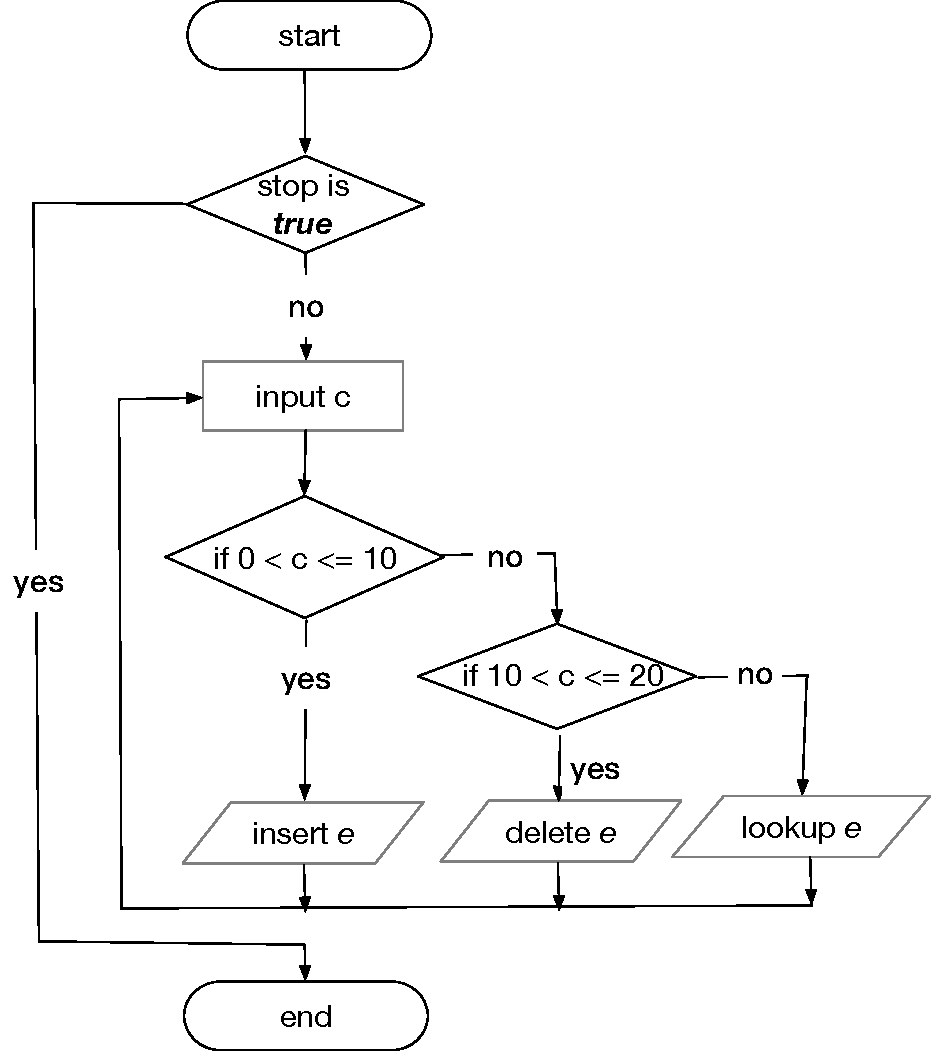
\includegraphics[width=0.9\textwidth]{flowchart_test}
\caption{CHTBench测试流程图}\label{fig:flowchart}
\end{figure}

如图~\ref{fig:flowchart}所示,
进入测试函数后,先判断此次执行哪种操作。
这个由随机值\textit{c}控制。
下面举例说明。
假设测试集中更新所占比重为20\%,则插入和删除各占10\%,而查询操作所占的比重为80\%,如果0 < \textit{c} <= 10时,执行插入操作;10< \textit{c} <= 20执行删除操作;而\textit{c}为其他值时则执行查询操作。

为了统计执行的总的操作次数,以及各项操作执行成功和失败的次数,每执行完一次操作,相应的计数器加1。最终通过统计相关计数器的值再除以执行时间得到吞吐量。

\section{本章小结}

%   \chapter{基于多核系统的并发哈希表的评估与分析}
\label{chap:chts}

计算机多核处理器技术的发展为处理更为复杂的数据创造了可能的同时,也为如何通过设计或者优化新的并发数据结构来充分发挥多核系统的性能特性提出了挑战。

在这一章中,首先对与本文密切相关的基本概念进行介绍,随后对现有的几类主要的哈希表进行描述,介绍相关参数的意义以及配置方法,最后给出对现有几个具有代表性的并发哈希表进行评估结果,以及通过对实验结果进行分析给出的并发哈希表设计和应用的最佳实践建议。

\section{实现并发哈希表的方法比较}

对于所有并发数据结构而言,断言并发访问是一项必要工作。
为了保证多个线程能够有序的对内存进行访问,有基于锁(lock-based)、无锁化编程(lock-free)和事务内存(transaction memory)几种主要的并发编程模型。

为了保证线程安全性,基于锁的并发哈希表对临界区进行加锁操作。
被锁保护的内存区间称为\textbf{临界区}(critical section)。
根据临界区的长短,基于锁的方法又可以划分为粗粒度(coarse-grained)锁实现和细粒度(fine-grained)锁实现。

一般的粗粒度锁在实现上相对简单,它使用少量的锁将受保护的数据结构分成几个区间,极端的情况是整个数据结构用一个全局锁。
这就使得临界区往往特别长,造成数据冲突的概率极高,不利于计算机资源的高效利用。
细粒度锁方法是使用锁对数据结构中的基本单元进行保护。比如哈希表中每个哈希桶设置一个锁字段对哈希桶进行保护,这样只有当不同的线程同时访问同一个哈希桶时才会造成冲突。
细粒度锁方法的好处是允许多个线程对数据的不同区段进行并发的读/写,大大提高了处理能力和资源利用率。
锁的粒度越细,越有利于提升整体性能,但是同时设计基于细粒度锁的数据结构的复杂度更高,并且正确性也难以得到保障。
同时使用大量的锁占用的存储空间也不容忽视。

无锁化编程是相对于基于锁的编程范式而言。
无锁化编程是用计算机原语来代替显示锁的一种并发编程范式。
同样的,无锁并发哈希也得到广泛的研究~\cite{urcu, nonblocking,metreveli2012cphash}。
使用无锁化编程设计并发数据结构能够获得良好的线程扩展性和性能。
但是,使用这种设计方法的复杂度不亚于细粒度锁实现。

事务内存的概念是沿用数据库事务处理的概念,数据库事务秉承ACID原则,即事务具有原子性,一致性,隔离性和持久性。
事务内存也遵循ACID原则:
\begin{itemize}
  \item 原子性:事务代码要么全部执行,要么全部不执行,不存在事务停滞在中间的某个状态,一旦因为某些原因需要中止,则事务回滚到事务开始执行的状态;
  \item 一致性:事务内存不会破坏数据的完整性和执行的事务代码的逻辑性;
  \item 隔离性:并行执行的多个事务代码区域互不干扰;
  \item 持久性:一旦事务代码成功执行完成提交,对系统状态所做的更改就会生效并且不会回滚,直到有新的事务执行结果对其进行修改。
\end{itemize}

事务内存的初衷便是让用户能够设计用粗粒度锁的实现方式获取接近甚至超过细粒度锁或无锁化编程的并发数据结构。目前,软件事务内存~\cite{todo}和硬件事务内存~\cite{todo}都得到了较好的实现。但是,在使用硬件事务内存是还需要使用软件优化方案,具体的细节将在下一章中详细介绍。


\section{典型的并发哈希表}

对串行哈希表的研究已日臻成熟,但是随着主流处理器生产商相继推出多核处理器之后,传统的串行哈希表已经无法充分利用多核系统的计算资源,也无法满足多核架构上的性能需求,在这样的背景下,相关研究人员开始着手高性能的并发哈希表的研究与设计。
并发哈希表继承了串行哈希表的快速索引,高效插入和删除元素的特性。
学术界和工业界的研究人员针对不同的应用场景提出并实现了一些具有特色的并发哈希表。
这些并发哈希表有基于用户态Read-copy Update(urcu)机制实现~\cite{urcu},
有被应用于memcached系统的多读单写Cuckoo哈希~\cite{memc3},
有应用于企业级应用的Threading Building Blocks (TBB)~\cite{tbb},
有集成到编程语言内的Concurrent\_HashMap~\cite{oracle},
\textcolor{red}{有使用消息传递机制来代替锁的CPhash~\cite{metreveli2012cphash}~.}
在哈希表密度非常高的情况下仍然可以保持较好性能的Hopscotch哈希~\cite{hopscotch},
以及遵循最小缓存行切换原则而以缓存行为哈希桶的缓存行哈希(CLHT)~\cite{clht}~等.

%所选哈希算法列表
\begin{table}[htbp]
  \caption{用于评估的五种并发哈希表实现}
\label{tab:concurrent_hash}
\footnotesize
\centering
\begin{tabular}{ccccc}
\toprule
序号 &   算法名称   &   设计思想     &   语言\\
\midrule
1  &  Cache Line Hash Table (CLHT)   &  Minimizes cache line transfers \cite{clht} &   C\\

2  &  Hopscotch Hashing (Hopscotch)   &  Combines the features of cuckoo, linear probing and chaining \cite{hopscotch}     &   C++ \\

3  &   Concurrent Cuckoo Hashing (Cuckoo)   &  A concurrent cuckoo hashing supports multi-reader/multi-wirter \cite{cuckoo}  &   C++ \\

4  &   User-Level Read-copy Update (URCU)   &   lock-free, trades update performance for read-side performance \cite{urcu}   &   C \\

5  &   Threading Building Block (TBB)   &   Based on separate chaining, scales well for read-heavy workload \cite{tbb}        &   C++ \\
\bottomrule
\end{tabular}
\end{table}

\subsection{缓存行哈希表}
\label{sec:clht}

T.David等人提出了一种“异步并发(ASCY)”的思想~\cite{clht},他们提倡遵循异步并发的四条编程模式来进行CSDS的设计。四条ASCY的编程模式内容如下:
\begin{itemize}
\item \textbf{ASCY$_1$}:CSDS的搜索操作不应该包含任何等待、重试或者存储;
\item \textbf{ASCY$_2$}:更新操作的解析阶段不应该包含任何重试或者等待,除非有清除当前内容的需要,否则不应包含任何存储;
\item \textbf{ASCY$_3$}:当某个更新操作在解析阶段失败之后(比如,需要删除某个元素使没有在哈希表内发现该元素或者在插入元素时发现该元素已经存在于哈希表内)不应当执行任何存储操作,除非有必要对解析阶段产生的数据进行清理;
\item \textbf{ASCY$_4$}:在成功的更新操作中进行内存存储的次数和存储的区域应当尽量与标准串行实现方法所消耗的次数和区域相近。
\end{itemize}

频繁的缓存行切换对并发哈希表的性能是灾难性的。
明确了这一事实后,T.David等人在四条异步并发模式的基础之上设计了缓存行哈希表(CLHT)~\cite{clht}。
CLHT的核心思想在于“并发算法想要获得良好的可移植性和可扩展性,它对于共享状态的内存的访问就需要像串行化那样是异步进行的。”
CLHT首要的设计准则就是“尽最大可能的缓存行的切换”,在这一准则下设计出的CLHT展现出极佳的性能。
为了确保大部分操作都能在一次缓存行切换内完成,CLHT的桶被精心的设计成与缓存行相同大小(64 Bytes,一般处理的缓存行大小都为64 Bytes)。
CLHT的冲突处理使用的是开链法,它的哈希桶通过指针链接。
因此,CLHT的哈希桶被隔离成8个字节,其中一个字节用于进行并发控制,6个字节用于存储三组键/值对,另外的一个字节用于指向其他桶。
基于这种哈希桶的结构设计基于锁的缓存行哈希方便。
直观的,完成一次更新操作(比如,在哈希表中插入新的元素),至少需要执行一次对共享状态的修改。

然而,根据ASCY指出的原则,查询操作不应该包含任何的存储。
因此,CLHT的查询操作需要对跟当前键对应的哈希桶进行解析并且不经过任何同步就返回结果。
为了实现就地更新,对哈希桶的解析不单纯的是对键进行遍历,还要同时获取每个键/值对的快照。
该原子快照确保搜索操作在找到目标键之后,与该键对应的值被返回但不会涉及并发修改。

CLHT有基于锁(CLHT-lb)和无锁(CLHT-lf)两个版本,本文对两个版本都进行了评估。
CLHT-lb采用细粒度锁(每个哈希桶都有一个锁字段)完成对读者和写者的同步控制。
查询操作遍历键/值对,如果匹配,则返回值。
更新操作首先需要执行进行一次查询以确定该操作可以继续执行(如果插入元素时发现桶内已存在相同元素或者删除元素时发现桶内没有该元素则不进行下面的操作),如果可以继续执行,则持有该桶的锁,直到完成相应的更新操作,完成后释放锁。
如果当前映射到的哈希桶内已经没有足够的空间插入新的元素,则会选择使用指针字段链入一个新的哈希桶,或者触发哈希表扩张操作(resize)。

而对于CLHT-lf,为了保持其插入键/值对插入时的原子性,设计了一个\textit{snapshot\_t}的对象。
\textit{snapshot\_t}的大小为8字节,它包括一个4字节的版本号和一个4字节的map。
\textit{snapshot\_t}提供在map内原子的读取/更改索引值的接口。
\textcolor{red}{版本号被用于原子的读取/更改map内的其他点。}
简而言之,CLHT-lf的原子性的过程可以大致描述如下:首先,通过在原子区间之前读取\textit{snapshot\_t}对象的值;
然后,使用比较并交换(CAS)原子指令对map内的目标索引值进行读取/更改。
举个例子,如果其他线程执行的并发插入已经完成了,那么当前的线程就会使CAS失败,因为两次的版本号不一致。
然后,可以通过map内的置位情况来判断给定的键/值对是处于有效、失效还是正在被插入三种状态中的哪一种。

\subsection{Cuckoo哈希表}
与CLHT所不同的是,Cuckoo哈希方法使用的开放寻址法解决哈希值冲突的问题。
使用的冲突处理方式不同注定了它们两者在数据结构上的差异。
Cuckoo哈希表中,所有的键/值对都被存放到一个大数组内,没有指针也不使用链表。
为了处理哈希冲突,它使用了两种技术:
\begin{itemize}
\item 第一,元素可以插入到桶数组内的两个位置(设置了两个哈希函数),如果其中一个位置被占用,则尝试插入到另外的位置上;
\item 第二,哈希桶设计采用多路组相连的方式,也就是说,对于每个桶都有B个“槽位(slot)”可供元素插入。
%为每一个键/值对提供两个哈希桶,如果当前哈希桶没有空闲位置供键/值对插入,则原来存储在这个位置的键/值对将会被踢出去,继续去寻找空闲的可供插入的位置,直到找到合适的位置或者达到预定的查找次数之后停止;
\end{itemize}

查找键k时,分别由哈希函数f$_1$和f$_2$计算得到k的两个可供k存储的位置b$_1$和b$_2$,然后在b$_1$和b$_2$的所有槽位中检查k是否存在。
图~\ref{fig:cuckoo}给出了一个使用2个哈希函数,4路组相联的Cuckoo哈希表。
采用这种设计带来的好处是:只需要检查2x4个键就能完成一次查询操作。因此查询操作非常快速并且是可预测的。
而在哈希表内插入新键时,如果b$_1$和b$_2$中任意一个桶内有空的槽位,那么就将该键存到这个桶内;
如果两个对应的桶都没有空闲位置,则随机的从带插入的桶内选择一个键踢出去,然后新的键插入到被踢出去的键的位置上。
被踢出的键则重新计算候选位置,可能会踢出其他的键以供自己插入,如此往复,直到没键被踢出或者达到预先设定的最大踢出次数为止。
如果最终仍有键没有找到空闲的位置进行插入,则说明哈希表的填充率接近极限了,此时会考虑对哈希表进行扩容操作。
一般的做法是将哈希表的容量扩大一倍,然后从扩容前的表中将数据拷贝到新创建的哈希表中。
在执行插入操作的过程中,被踢出的键序列被称作一条Cuckoo路径。
当表的填充率升高时,Cuckoo路径的长度会增加,没执行一次插入所需要的随机读/写的次数也会增加,Cuckoo的更新性能也因此受到影响而下降。

Cuckoo hashing方法最早是由R.Pagh等人在2004年提出的~\cite{cuckoo-src},其原始版本并不支持多线程并发。
之后由X.Li~\cite{memc3}和B.Fan~\cite{cuckoo}等人分别实现了支持多读单写和多读多写的并发Cuckoo哈希表。
本文中使用的B.Fan等人实现的多读多写Cuckoo哈希表。

%cuckoo数据结构
\begin{figure}[htbp]
\centering
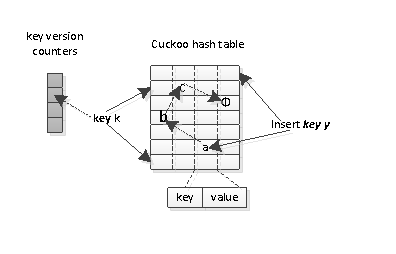
\includegraphics[width=0.9\textwidth]{cuckoo}
\caption{4路组相联Cuckoo哈希表}\label{fig:cuckoo}
\end{figure}

\subsection{Hopscotch哈希表}
与Cuckoo类似,Hopscotch也是采用的开放寻址法解决哈希冲突问题。
它在设计时综合考虑了Cuckoo哈希,线性探测法和链式法的特点,并将三者的优点结合起来。
Hopscotch哈希表由哈希桶数组构成。
它的核心概念在于任意的哈希表内的元素,它周围的所有哈希桶都称为其邻居哈希桶。
邻居哈希桶具有一个重要的特性:在邻居桶内查找元素所需的开销与在被映射的桶中查找元素所需的开销相同或者非常接近。
这个特性专门为处理插入操作而设计的。

图\ref{fig:hopscotch}实例描述Hopscotch插入元素的过程。
元素被映射进的实体总是在经过哈希函数计算得到的实体内或者在其相邻的下一个H-1实体内,其中H是设定的常量(一般H为32或者64位,一个标准机器字长),可以根据需求进行调整。
每一个实体包含一个字节的’跳‘信息和一张H比特的位图,位图指示在当前实体的下H-1个实体内包含该元素的虚拟桶的偏移量。
通过查看‘跳’信息能够得知哪些实体属于同一个哈希桶,然后只需扫描常数级别的实体数量快速的找到某一元素。
从任意相邻桶内找出某一特定元素的开销等同或者非常接近于直接从该元素所属的桶内进行查找的开销。


总之,Hopscotch的设计思想就是将空闲的槽位向着目标哈希桶移动,或者像Cuckoo哈希那样将元素从目标桶中移除然后重新为其寻找合适的位置。
Hopscotch实现了串行和并发两个版本~\cite{hopscotch},本文中用到的支持多线程并发的Hopscotch。

%cuckoo数据结构
\begin{figure}[htbp]
\centering
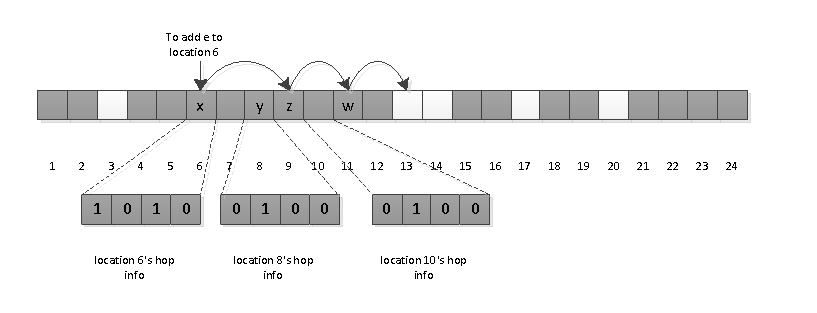
\includegraphics[width=0.9\textwidth]{hopscotch}
\caption{Hopscotch插入操作示例}
\label{fig:hopscotch}
\end{figure}

\subsection{基于RCU机制的哈希表}

\textcolor{red}{spilted-order list有基于URCU的实现版本,具体参看谷歌搜索urcu hash table的结果。}

读-复制更新,Read-copy Update(RCU)并不单纯是一种并发哈希表的设计方案,它最初是一种用于优化Linux系统内核的共享数据访问的一种并发模型~\cite{rcu}。
RCU是一种无锁化编程模型。
对于被RCU机制保护的共享数据结构,读者线程可以不需要锁自由的对其进行访问,但是写者线程在对该共享数据结构进行修改前必须保留该数据结构的副本。
当修改完成之后,通过适当的回调函数将指向旧数据的指针修改成指向新的数据(从旧数据拷贝的数据)。
RCU的核心概念有两个:一个成为静默期(quiescent state);一个称为优雅期(grace period).
\textcolor{red}{补充静默期和优雅期的描述与功能。}

基于RCU的并发哈希表的最大特点是牺牲更新性能来换取读性能。
基于RCU的编程模型主要用于Linux系统内核,为了便于将RCU集成到我们的测试框架下进行测试我们使用用户态的RCU实现(URCU)~\cite{urcu}~。
本文使用的URCU v-0.8.8版本~\cite{urcucode}。

\subsection{基于线程构建模块的哈希表}

Intel推出的线程构建模块(Threading Building Blocks, TBB)是一种针对多核平台的基于任务的并行编程模型~\cite{tbb}。
它实现的concurrent\_hash\_map允许多个线程并发的访问。
concurrent\_hash\_map的键是无序的。
每一个键在哈希表内最多只有一个元素与之相对应,但不排除有其它的元素尝试插入到相同位置。
类\textit{const\_accessor}和\textit{accessor}统称为访问控制器(accessor)。
访问控制器允许多个线程并发的访问哈希表内的键/值对。
访问控制器充当指向键/值对的智能指针。
它持有作用于键/值对上的隐式锁,直到该实例被销毁或者访问控制器调用解锁函数才会释放。

TBB实现的并发哈希表处理冲突采用的是典型的链式法。
键被哈希到包含了实体形成的链表的哈希桶内。
基于TBB的并发哈希表继承了链式法的所有优缺点。
适合处理读占多数的数据集。
本文中,将TBB v 4.2集成到CHTBench中进行测试。

\section{并发哈希表的评估与分析}
\textbf{并发哈希表}(CHT)是一种允许在同一时刻有多个读者或写者访问共享对象的哈希表。
其提供与串行哈希表一样的访问接口,但是CHT能够更有效的发挥多核处理器的性能。
并发哈希表的性能不仅依赖于应用本身的需求而且还依赖于底层硬件特性。
所以,对并发哈希表的剖析不能单纯的停留在吞吐量、延迟等直观的指标上,而是要综合考虑微观和宏观,底层和上层等多个层面的影响。
进一步说,选用通用的测试评估指标在一个统一的测试框架下进行测试,处理不同的工作集时没有任何一种并发哈希表能全面的体现其优势。
另一方面,对于用户而言,能够预先知道某种CHT的性能障碍将对其挑选合适的并发哈希表提供帮助。
不幸的是,这种用户关切的问题在现有研究中鲜有人提及。
由于缺乏一个统一的测试框架,用户也很难通过自行测试进行比较而选出理想的CHT应用到其软件系统中。
总之,对并发哈希表进行全面深入的剖析对并发哈希表的使用、设计以及优化都具有深远意义。
基于以上考虑,我们从现有的并发哈希表中挑选出表~\ref{tab:concurrent_hash}中列举的五种比较突出的进行深入的分析。

具体的,将挑选的CHTs放入CHTBench的框架内进行测试,对并发哈希表的评估与分析将围绕并发哈希表的线程扩展性、更新比重对性能的影响、初始化的哈希表元素的规模对性能的影响、延迟、线程绑定方案、同步机制以及内存消耗等七个方面展开。

\subsection{测试平台与配置}
为了体现对并发哈希表的评估具有一般性,测试在4台基于不同体系架构的多核处理器上展开。
它们分别是AMD Opteron 6172,Intel Xeon E5-2630,Xeon E7-4850,以及Intel Xeon Phi 7120p。
表~\ref{tab:arch_info}~给出了4个平台的硬件和系统特征。
测试过程中为了避免因操作系统的差异引入的干扰因素,所有测试平台都搭载Ubuntu 14.04 LTS操作系统。
下面分别对4台机器的硬件特征逐一进行介绍。

%目标平台的硬件和系统特征
\begin{table}[htbp]
  \centering
  \caption{测试目标平台的硬件和系统特征}
  \label{tab:arch_info}
  \begin{tabular}{ccccc}
    \toprule
       名称             & AMD Opteron           & Intel E5-2630       & Intel E5-4850     & Intel MIC \\
    \midrule
      系统               & Magny Cours      &  Ivy Bridge-EP        &  Haswell-EX         &  Knights Coner \\
      处理器             &  Opteron 6172         &  Xeon E5-2630      & Xeon E7-4850     &  Phi 7120P \\
      核/线程数量         & 24/48                & 16/32                & 48/96              & 61/244 \\
      时钟频率(GHz)       & 2.1                  & 2.4                  & 2.3               & 1.238 \\
      L1缓存(KB)         & 64/64 I/D             & 32/32 I/D            & 32/32 I/D         & 32/32 I/D \\
      L2缓存(KB)         & 512                  & 256                   & 256               & 512 \\
      LLC缓存(MB)        & 2x6                  & 20                    & 24                & NULL \\
      互联通道            & 6.4 GT/s HT          & 2x QPI               & 3x QPI             & NULL \\
      最大内存带宽(GB/s)   & 42.7                 & 51.2                 & 68                & 352   \\
      % 内存型号            &                       &                     &                   &         \\
      主存(GiB)         & 128                   & 56                  & 128                & 16 \\
    \bottomrule
  \end{tabular}
\end{table}

\begin{figure}[htbp]
\centering
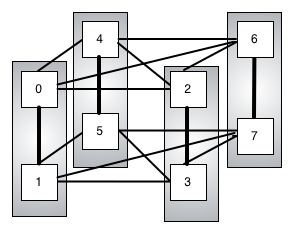
\includegraphics[width=0.6\textwidth]{AMD_top}
\caption{AMD Opteron内存结点拓扑结构}\label{fig:AMD_top}
\end{figure}

\textbf{AMD Opteron.} 该48核的AMD Opteron机器包含4个Opteron多芯片模块(MCMs)。
该系统总共具有八个内存结点:每一个MCM分为2个片区,每个片区拥有6个核,各个片区使用独立的内存控制器进行控制。该系统的拓扑结构如图~\ref{fig:AMD_top}~所示。
位于同一个多芯片模块内的两个片区之间的距离定义为1跳(1-hop),位于不同多芯片模块上的两个片区距离为2跳(2-hop)。
多芯片模块内通信开销要低于多芯片模块间的通信开销,并且模块内的两个片区之间的共享带宽比位于两个不同模块内的片区间的共享带宽要高。
它的CPU的时钟频率为2.1 GHz,三级缓存的容量分别为64 KiB,512 KiB和4 MiB (每一个片区的私有缓存容量)。
总的运行内存为128 GiB。
Opteron的缓存具有回写和非包容性~\cite{Conway2010Cache}。
然而,存储的层次结构并不具备严格的排他性,也就是说在LLC中命中的数据会被推送到L1中,至于该数据会不会在LLC中被删除取决于硬件实现~\cite{2011Software}.
Opteron采用MESI的扩展性协议MOESI作为缓存一致性协议。
其中’O’表示占有(Owned)状态,它表示缓存行的内容被修改,与内存中的数据不一致,不过在其他的核上可能有这份数据的副本。

\textbf{Intel Xeon E5-2630.} Intel Xeon E5-2630由两路插槽组成,每路插槽中有8个物理核(16个硬件线程),它的运行内存为16 GiB。
它的时钟频率为2.4 GHz,三级缓存的容量为别为32 KiB,256 KiB 和20 MiB。
该系统具有4个内存通道和两条6.4 GT/s的快速互联通道(QuickPath Interconnect, QPI)。
E5-2630的最大内存带宽可达59 GB每秒。
它的缓存具有包容性,即就是说每一个新的缓存行的填充都将在三级缓存中同步~\cite{intel2016}。
最后一级缓存是回写的,当出现由空间不足或者一致性问题引起处于‘M’状态的缓存行被驱逐时,数据被写入到内存中。

\textbf{Intel Xeon E7-4850.} 该平台由4个插槽组成,每个插槽内有12个物理核(24硬件线程),它的运行内存为128 GB,时钟频率为2.3 GHz。
它的三级缓存的容量分别为32 KB,256 KB和24 MB。
它具有4个内存通道和3个QPI。
该机器的最大内存带宽为68 GB每秒。
它采用的缓存一致性协议与E5-2630相同.

\textbf{Intel Xeon Phi 7120p.} 该机器在同一片芯片上集成了64个有序内核。
每一个内核均支持最多四个硬件线程,因此该机器的最大硬件线程数量可达244个之多,单个内核的时钟频率为1.23 GHz。
Intel Xeon Phi 7120p的内存分层结构类似于传统的多核系统。图~\ref{fig:phi_arch}~所示为其体系结构.
Phi上的内存为所有核所共享,所有的内核均可对其进行访问,该机器的内存大小为16GB。每一个核都有一个大小为32KB的一级数据缓存和32KB的一级指令缓存,以及一个大小为512KB的二级私有缓存,片上二级缓存的总量为31MB。
Phi实现了一个扩展的MESI协议,该协议的新颖性在于其将Shared状态扩展为一个基于目录的缓存一致性协议,这个协议简称为GOLS(Globally, Owned, Locally Shared),该协议的好处是能够共享被修改的缓存行,并且避免地址总线上的广播风暴。
每一次的缓存都通过查看GOLS协议来确定缓存行的状态。Phi的全局一致性的维护是通过纪录有每一个缓存行一致性状态的分布式目录标签(Distributed Tag Directories, DTDs)完成的。每一个缓存行的地址都通过一个哈希函数映射到DTD上,这样做的好处是保证负载均匀分布。

\subsection{线程扩展性}

线程扩展性是指在多核平台上随着被创建的线程数量的增加,应用的吞吐量保持不减的趋势。
线程扩展性直观的体现在吞吐量上,吞吐量也是很常用的性能评价指标之一。
吞吐量的计算方式用执行的哈希表查询、插入和删除操作的总和除以执行完成这些操作所耗费的时间。
单位用百万操作每秒(Mops/s)表示。

\label{sec:thread_scal}
\subsubsection{总体的扩展性评估}

本次实验中,采用紧凑的线程绑定方案(具体见~\ref{sec:thread_pinning}~),每次测试的持续时间为5秒,实验的结果如图~\ref{fig:thread_scal}~所示,每一组参数配置都运行五次,最终结果取五次结果的平均值。

从图~\ref{fig:thread_scal}~的曲线变化可以观察到,在这样的参数配置下,URCU在多个平台上的吞吐量曲线几乎与x轴重合,也就是说在更新比重为10\%的情况下,URCU的性能很糟糕。
而CLHT(由于CLHT-lb和CLHT-lf之间的趋势相同,数值接近,故不单独进行讨论)则在4个平台上均展现出最佳的性能,这得益于它的设计出发点:尽可能的减少缓存行的切换次数。
Hopscotch的吞吐量在E5-2630和E7-4850两台机器上达到峰值时对应的线程数分别为16和24.值得注意的是,16和24正是这两台机器单个内存结点(socket)支持的最大线程的数量。
同样的它在AMD Opteron上的峰值出现在线程数为6这个点(6恰好是该机器同一片区支持的最大线程数)。
综合Hopscotch在三个NUMA架构平台上的表现,可以推断Hopscotch在降低跨内存结点通信开销方面存在缺陷,它在单内存结点的多核计算机平台上应该有不错的线程扩展性。
换句话说就是Hopscotch在利用NUMA系统特性上所做的优化粒度不够,更多的细节描述见~\ref{sec:thread_pinning}~节。

%Intel Phi 7120p 体系结构
\begin{figure}[htbp]
\centering
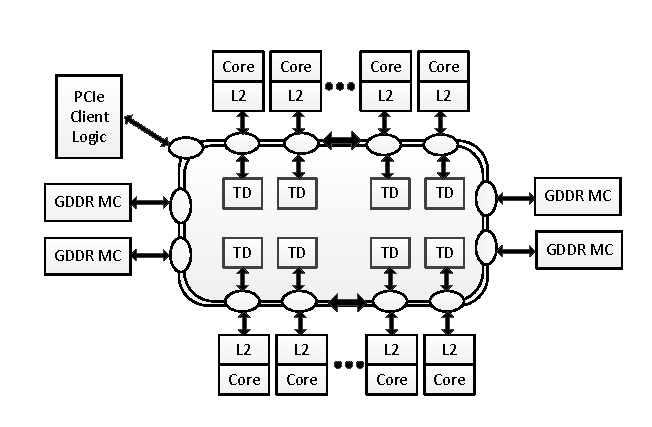
\includegraphics[width=0.9\textwidth]{PHIarch}
\caption{Intel Phi 7120p体系结构}\label{fig:phi_arch}
\end{figure}

考虑到在图~\ref{fig:thread_scal}~(a)中当线程数为16时存在一处拐点,故将该平台上的性能曲线单独分成两个阶段进行说明。

\textbf{阶段1}:在这个阶段创建的线程数量在1到16这个范围内,超线程没有被启用(紧凑型线程绑定方案)。
很明显CLHT表现出最佳的吞吐量增长速率,每多创建一个线程,它的吞吐量大约增加15 Mops/s。
CLHT-lb的性能优于CLHT-lf版本。对Hopscotch而言,每多创建一个线程,吞吐量大约增加5.5Mops/s. 在该阶段Cuckoo的性能比TBB要差。

\textbf{阶段2}:在这个阶段,创建的线程数量大于16个,线程分布在两个不同的插槽内而且超线程在这个阶段也被启用参与运算。
可能受到内存带宽上限的影响,CLHT的吞吐量保持微弱的增长势头。表~\ref{tab:mem_bandwidth}~列出了在Intel Xeon E5-2630平台上CLHT-lb的内存带宽随着线程数量的变化情况。
该表中数据表明在该阶段CLHT-lb运行时内存带宽没有发生变化。
而Hopscotch性能的陡然下降揭示它在处理跨插槽通信上的性能开销远大于增加额外的线程带来的性能增益。在这个阶段Cuckoo和TBB展现出不错的增长速度。

%表2,内存带宽使用情况
\begin{table}[htbp]
  \centering
  \caption{CLHT-lb内存带宽随线程数量变化情况}
  \label{tab:mem_bandwidth}
  \begin{tabular}{cccccccccc}
    \toprule
       Threads & 1 & 4 & 8 & 12 & 16 & 20 & 24 & 28 & 32 \\
    \midrule
      内存带宽(单位:GB/s) & 1.5 & 5.8 & 11.2 & 12.8 & 12.8 & 12.8 & 12.8 & 12.8 & 12.8 \\ 
    \bottomrule
  \end{tabular}
\end{table}


\begin{figure}[htbp]
\centering
%\subfigure[Intel]{
\subfigure[E5-2630]{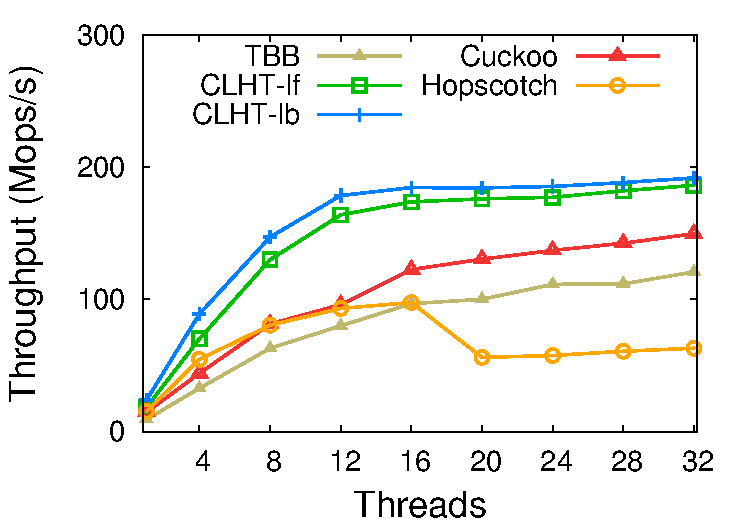
\includegraphics[width=0.45\textwidth]{2630Scal}}
\subfigure[E7-4850]{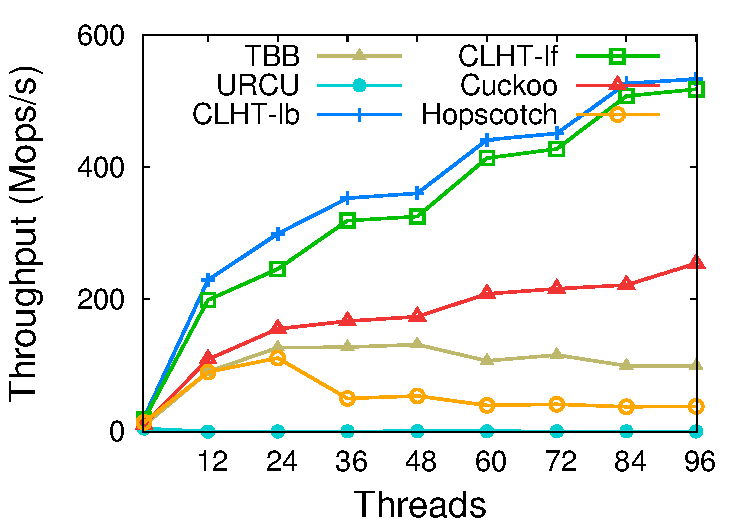
\includegraphics[width=0.45\textwidth]{4850Scal}}
\subfigure[Opteron]{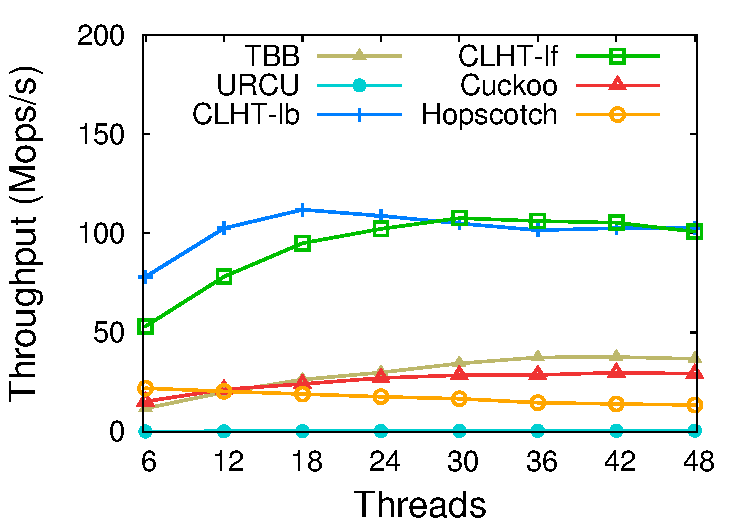
\includegraphics[width=0.45\textwidth]{AMDScal}}
\subfigure[Phi 7120P]{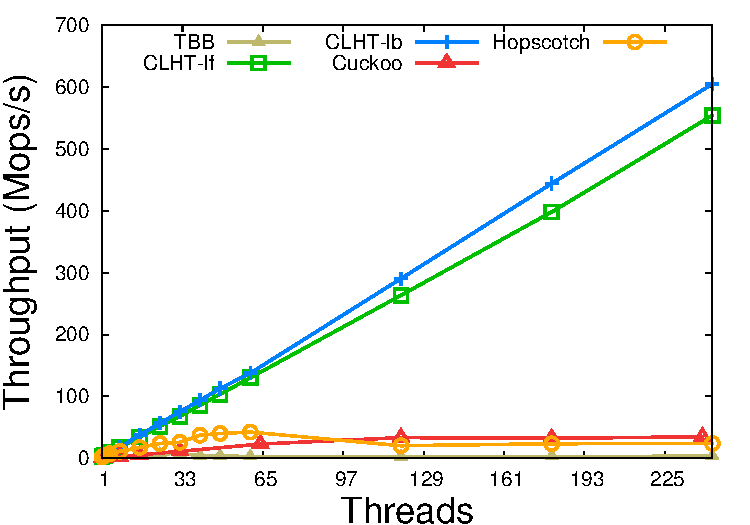
\includegraphics[width=0.45\textwidth]{7120PScal}}
\caption{并发哈希表的吞吐量随线程数量的变化曲线,哈希表的密度为50\%,\textit{u}为10\%,\textit{i}为一百万。}
\label{fig:thread_scal}
\end{figure}

图~\ref{fig:thread_scal}~(b)刻画的是E7-4850平台上的吞吐量曲线。
除CLHT之外,其它几种并发哈希表的性能曲线走势与E5-2630相似。
前面介绍了在E5-2630平台上由于受到内存带宽的限制,CLHT的吞吐量在第二阶段基本没有增长,而在E7-4850平台上CLHT全程保持稳定的增长趋势。

图~\ref{fig:thread_scal}~(c)给出的是AMD机器上的运行结果。
在该机器上TBB的线程扩展性在5个并发哈希表中仅次于CLHT。
Hopscotch只有当线程分布在同一个片区内时(n<=6)才具备最佳性能,创建更多的线程并不能促进整体性能的提升。
另外,对于Cuckoo和CLHT,当创建的线程数量超过某个特定的值时,会引起吞吐量的下降,这种引起吞吐量下降的原因来自两个方面:一是受到内存带宽的限制;一是来自有限的资源被多个线程激烈竞争。

Xeon Phi 7120P上的实验结果如图~\ref{fig:thread_scal}~(d)所示。
CLHT的两个版本在该平台上获得了线性的线程扩展性,每多创建一个线程,相应的吞吐量会增加大约2.5Mops/s. 
CLHT在该平台上获得线性扩展性归因于两个方面:
其一,每一个哈希桶的大小等于缓存行的大小,这样大大降低了缓存行切换的次数。
并且数据对齐有利于避免多线程伪共享问题,多线程伪共享是影响Xeon Phi性能的主要因素之一。
其二,CLHT采用细粒度锁在一定程度上抑制了线程间的竞争。
然而,并不是所有的并发哈希表在Phi 7120上都能表现的如CLHT一般呈现线性扩展性,相比于其它几个平台Cuckoo和TBB在该平台上的性能非常差,创建更多的线程也无法保证性能的提升。详细的原因将在~\ref{sec:impact_update}~和\ref{sec:sync}节中阐述。

\subsubsection{数据分布方式对线程扩展性的影响}
在前面的实验中,键值对是用随机方法产生的,服从均匀分布。
但是在实际的应用场景下,数据完美的均匀分布只存在理想状态中,某些数据出现的频度存在两极分化,因此,人们会更加关注不同的数据分布形式下各哈希表的性能表现。
在这一部分内容中,我们将对服从zipf分布的数据集进行测试。
在本次测试中,参数配置比如哈希表密度,更新比重以及哈希表的初始化元素个数均与线程扩展性一节的参数设置保持一致。
图~\ref{fig:zipf}为运行服从zipf分布数据集的性能曲线(在几个平台上的性能变化趋势相一致,故我们只给出了在E5-2630上的实验结果)。
与图~\ref{fig:thread_scal}(a)中的实验结果进行比较,Cuckoo,CLHT,Hopscotch以及TBB的吞吐量分别下降44\%,51\%,53\%和30\%。
性能下降的原因在于zipf分布使得数据访问更加倾向于频度较高的键值对,造成多数的操作集中访问少数频度较高的数据内容。
这加剧了多个线程访问相同键的竞争程度,对片上互联通道和同步造成压力从而引发更多的缓存一致性流量。

%数据服从zipf分布时,CLHT-lb的线程扩展性
\begin{figure}[htbp]
\centering
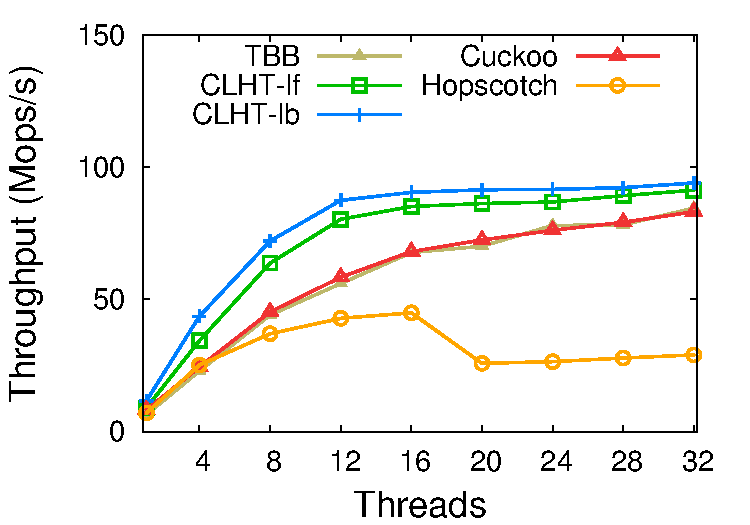
\includegraphics[width=0.6\textwidth]{2630zipf}
\caption{数据服从zipf分布时吞吐量随线程变化情况}
\label{fig:zipf}
\end{figure}

\subsubsection{哈希表的扩张}
不断的往哈希表中插入新的元素会引起哈希表密度的增加,将导致插入元素的时间成本增加。
在最坏的情况下,会因为找不到空闲位置并尝试多次之后导致插入操作失败,这无疑会对哈希表的性能造成巨大的损耗。
面对这样一种情形,大部分哈希表在设计的时候允许哈希表在达到一定密度后自行进行扩张。
具体的工作流程是,创建一张新的哈希表,新表的容量一般为旧表容量的两倍,然后将旧表中的元素拷贝到新表中,这不可避免的引入额外的时间和空间开销。
为了探究并发哈希表进行扩张时的开销情况,设计了如下一组实验。
在本次测试中,由于Hopscotch不支持哈希表的扩张,故没有比较,哈希表的初始化密度设为90\%,更新比重调整为40\%,其中插入占35\%,删除占5\%,这样设计的目的在于确保插入表中元素的个数大于被删除的元素个数,从而保证在运行过程中哈希表中元素的密度在不断的增加,增加触发哈希表扩张的概率。
实验结果表明,Cuckoo触发resize操作的概率低于TBB和CLHT,我们认为这得益于Cuckoo在查找cuckoo路径上所做的优化。在触发哈希表扩张操作的情况下,吞吐量大概下降5\%左右。

\textbf{分析}:创建更多的线程并不总是意味着吞吐量的增加。
一方面,创建更多的线程可能导致内存子系统达到饱和,从而导致性能不再上升甚至将削弱总体性能。
另一方面,NUMA系统在缺乏适当仲裁机制的情况下更高的并发度将引起高速互联通道的竞争居高不下,从而达不到最优性能。与传统的多核架构相比,Intel MIC架构在并发哈希的扩展性方面体现出重大差异。
在这种新的体系架构平台上设计并发哈希表需要充分考虑改种体系架构的特征。
处理倾向于高频度数据的访问的工作负载将引起更高的缓存一致性流量,这将需要更复杂的同步算法来缓解性能下降的问题。

\subsection{更新比重对性能的影响}
\label{sec:impact_update}
并发哈希表与串行哈希表一样善于处理读操作占多数的工作负载。
在本节中,通过调整工作负载中更新操作的比重来观察各个并发哈希表性能的变化情况。
哈希表中初始化元素的个数设置为一百万。
在三个NUMA架构平台上,选取\textit{n}为平台单个socket支持的最大线程数。
Phi 7120P上\textit{n}是选取一个能够展示线程扩展性的值。
这样,使用紧凑型线程绑定策略时可以避免跨socket流量的干扰。

\begin{figure}[htbp]
\centering
%\subfigure[Intel]{
\subfigure[E5-2630, n = 16]{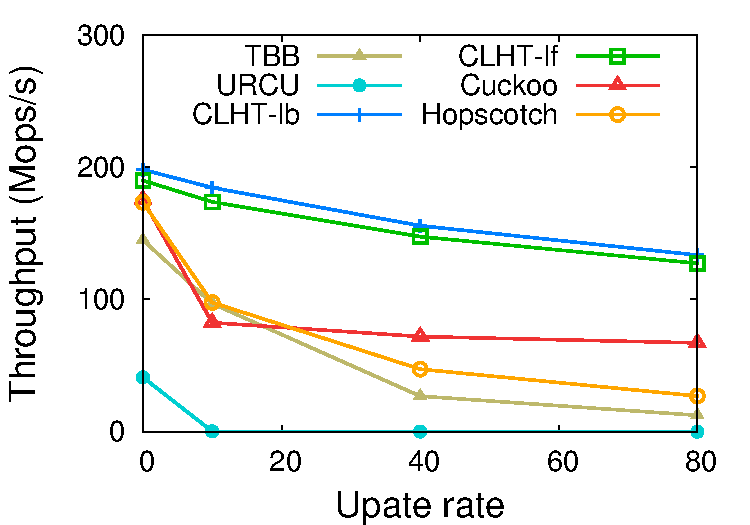
\includegraphics[width=0.45\textwidth]{2630Update}}
\subfigure[E7-4850, n = 24]{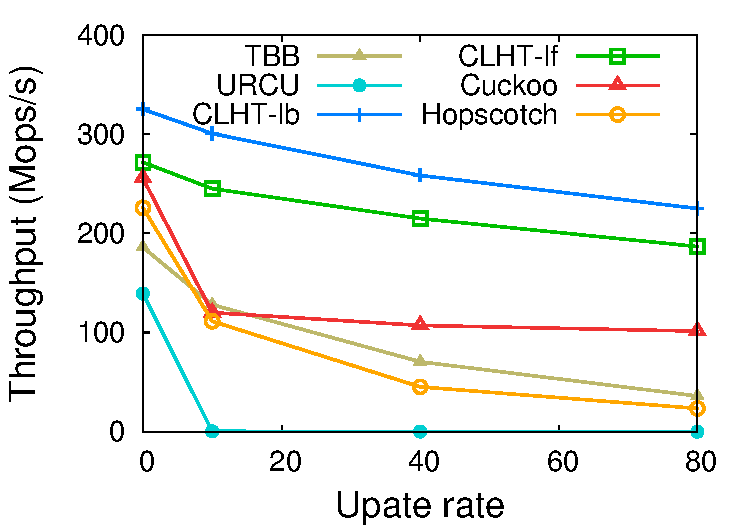
\includegraphics[width=0.45\textwidth]{4850Update}}
\subfigure[Opteron, n = 12]{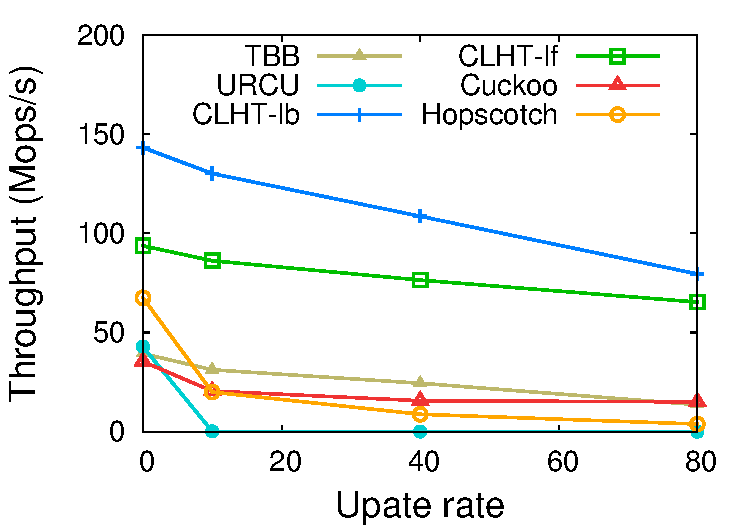
\includegraphics[width=0.45\textwidth]{AMDUpdate}}
\subfigure[Phi 7120P, n = 60]{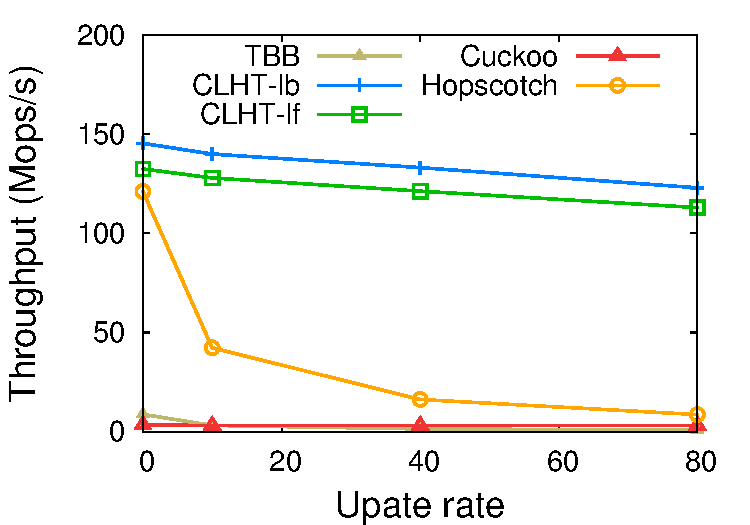
\includegraphics[width=0.45\textwidth]{7120U10}}
\caption{哈希表初始化元素个数一定的前提下,吞吐量随更新比重变化趋势}
\label{fig:update}
\end{figure}

如图~\ref{fig:update}~所示,
所有的并发哈希表的吞吐量峰值都出现在更新比重为0处,也就是说并发哈希表对处理纯读的工作负载具有最佳性能。
但是一旦运行的工作负载中包含了更新操作,性能会有很明显的下降。
其中URCU对于更新操作最敏感,更新比重从0调整到10\%,URCU的吞吐量下降到原来的1/270。下降幅度大的还有Hopscotch。
该现象同样解释了Hopscotch由于很高的同步开销导致的严重的扩展性问题(其它的并发哈希表比如TBB和URCU也有同样的问题)。
在更新比重增加时,Cuckoo表现出相对稳定的性能,它的下降速率在几个并发哈希表中是最低的,表明Cuckoo更能应对具有高更新比重的工作负载。

为了更好的说明工作负载中的更新比重发生变化引起性能变化的原因,本次实验引入一个新的微观指标:缓存未命中数/总的操作数量。
缓存未命中数用VTune Amplifier进行测量,测量结果为线程数16时的结果,具体见表~\ref{tab:cache_miss_update}。
通过表3的数据表明工作负载中更新比重越高,每操作对应的缓存未命中数也越高。
CLHT在低更新比重和高更新比重下都表现良好,这从表3中也可以得到体现,CLHT对应的最大值与最小值之间的差距只有30\%。
而URCU对应的值从0到10\%这个阶段扩大了14倍,从0到80\%更是扩大了127倍之多。
糟糕的情况更不止如此,URCU的CPU利用率非常低,大约保持在3\%左右,而同等参数配置下其它并发哈希表的CPU利用率达到50\%。进一步探究发现,
创建更多的线程并不会引起缓存未命中数量的增加,这表明工作负载中更新比重的变化是引起吞吐量变化的主要原因。

%表3,调整更新比重时缓存未命中率的变化情况
\begin{table}[htbp]
  \centering
  \caption{平均缓存未命中数量随更新比重变化情况}
  \label{tab:cache_misses_update}
  \begin{tabular}{ccccccc}
    \toprule
       更新比重(\%) & TBB & URCU & CLHT-lf & CLHT-lb & Cuckoo & Hopscotch  \\
    \midrule
     0 & 28.6 & 85.2 & 23.6 & 31.7 & 33.5 & 22.9  \\
      10 & 46.3 & 1169.2 & 24.6 & 34.9 & 44.2 & 28.1 \\
      40 & 99.2 & 4046 & 27 & 37.3 & 57.2 & 62.7 \\
      80 & 159.1 & 10788 & 30.7 & 40.6 & 66.2 & 115.5  \\
    \bottomrule
  \end{tabular}
\end{table}

\textbf{分析}:频繁的缓存行切换是并发哈希表更新性能最大的敌人。
更新操作致使缓存行失效的原因来自于两方面:一方面是写入本地内存结点的流量;另一方面是被缓存一致性协议强制进行的跨socket消息以及通过片上高速互联通道如Intel QPI和AMD HyperTransport等传递的信息。
一些设计用于处理读为主的工作负载的并发哈希表,哪怕是工作负载中包含很小部分的更新操作,它的性能也会大打折扣。
写友好型并发哈希表通常会进行精心设计用以控制缓存内的关键数据,比如共享变量等。

\subsection{缓存与主存}
考虑到哈希表属于内存密集型应用,所以在这一部分我们探究内存分层结构对并发哈希表性能的影响。
图~\ref{fig:initial_size}中的柱状图表示吞吐量随着哈希表初始化元素个数的变化情况,不同的初始化值所需的内存对应相应平台的三级缓存容量与主存容量。

\begin{figure}[htbp]
\centering
%\subfigure[Intel]{
\subfigure[E5-2630]{\includegraphics[width=0.45\textwidth]{2630Init}}
\subfigure[E7-4850]{\includegraphics[width=0.45\textwidth]{4850Init}}
\subfigure[Opteron]{\includegraphics[width=0.45\textwidth]{AMDInit}}
\subfigure[Phi 7120P]{\includegraphics[width=0.45\textwidth]{7120PInit}}
\caption{不同初始化大小对应的吞吐量抽样直方图}
\label{fig:initial_size}
\end{figure}

由于Phi 7120P与其它三个平台在内存分层结构上存在差异,故单独列出讨论。
从图~\ref{fig:initial_size}~(a)-(c)中观察到,当工作集的规模小于缓存的容量时,吞吐量是随着初始化大小增加的。
我们通过likwid-perfctr这个工具对最后一级缓存与主存之间的带宽与流量进行监测确认了这一结果。
一旦工作集的规模超过最后一级缓存的容量,将有较大的性能损耗。
此外,CLHT由于其在缓存使用机制上的独特设计,它的工作集规模小于缓存容量时的性能要比其它方法更好。
通过本次实验,我们还观察到一个有意思的现象(图~\ref{fig:initial_size}中没有体现该现象),当被创建的线程个数增加时,在一级缓存中存在显著的数据竞争情况。
下面通过举例对此现象加以说明,当初始化元素个数为1000时,并发哈希的吞吐量随着线程数量的增加而降低。
这个现象的原因在于线程越多,不同线程同时访问相同的共享数据的概率越高,从而导致较高的同步开销。

Hopscotch在本次实验中属于例外情况,它的吞吐量几乎不随初始化元素个数的变化而变化。
进一步的探究发现在Hopscotch的实现中,哈希表的内存是通过预先开辟固定大小的内存空间建立的。
这种方法的好处是获得了性能的稳定,缺点是丧失灵活性,在处理较小规模的工作负载时对内存空间的浪费较严重。
对高并发度的应用而言,无论是基于锁还是无锁的并发哈希表的实现,都依赖于有效的内存管理机制。而这些内存管理机制通常是建立在第三方插件的基础之上,或者来自由系统提供的动态内存分配器。
需要说明的是,有些并发哈希表在试图运行更大的工作负载(初始化值大于1亿)时失败了。这也可能是由内存管理上的缺陷造成的。

前文中指出,Phi 7120P的内存分层结构于其它主流多核体系架构存在较大差异。
它只包含两级缓存,并且其核与内存控制器之间是通过双向环状总线进行连接的。图~\ref{fig:initial_size}~(d)为Phi 7120P上的实验结果,在该平台上CLHT的吞吐量随着初始化元素个数的增加而降低,而其它几种哈希表因为数值太小在图中无法明确的体现这一趋势,通过比较实验数据发现同样符合这个趋势。

除了图~\ref{fig:initial_size}~中展示的数据规模之外,还对运行超过GB级别的数据进行了测试。
性能曲线与初始化值为一百万时的同类测试类似,只是在吞吐量上要打折扣。

\textbf{分析}:缓存对加速不同体系架构的性能具有非常重要的作用。
对缓存采用细粒度的方法进行控制的目的在于获得可预测的结果,比如为常驻缓存的工作集进行线程调度有利于避免额外的同步开销。
静态内存分配的方式对于并发哈希这种内存密集型应用来说并不是最佳选择,而对超大规模数据集使用动态内存分配方式需要进一步的优化方案予以辅助。

\subsection{操作延迟}
\label{sec:latency}
前文从宏观的吞吐量出发对并发哈希表进行了评估,在这一节当中我们从微观的每个操作执行的运行时延迟的角度进行分析。
对于延迟敏感型应用而言,理解不同算法设计的延迟变化造成的影响至关重要。

本次实验中,更新比重设置为10\%,哈希表密度为0.5,哈希表的初始化元素个数为一百万。
通过实验收集哈希表操作所耗费的CPU时钟周期数进行统计。
我们对哈希表的操作进行如下定义:如果某个操作完成了对其预期目标对象的访问,我们称该次操作为一次成功的操作;否则我们称之为一次失败的操作.
根据如上定义,得到六种不同的操作类型,它们分别记做:get-suc, get-fail, put-suc, put-fail, rem-suc和rem-fail。所需的时钟周期数使用开源工具sspfd~\cite{sspfd}~收集,然后通过均匀抽样方法计算每种操作对应的平均延迟。

图~\ref{fig:latency}给出了我们在E5-2630平台上的实验结果。
随着所创建的线程数量的增加,资源的竞争(包括内存带宽,缓存以及内存控制器)和同步开销逐步增加,这些都将不可避免的导致延迟的增加。
通过比较发现,CLHT(两个版本)在大部分情况下的延迟都低于其它并发哈希方法,这归因于它在设计上严格遵循4条异步并发模式。
过多的缓存行切换需要更周密的缓存一致性协议予以支持,从而导致哈希表操作延迟的增加。在几种并发哈希表中,URCU的操作延迟最高,原因是URCU在设计上有一个称为“RCU优雅时间”的等待期。Hopscotch的延迟对跨插槽通信相当敏感(对应图中线程数量大于8时的曲线变化)。
并且在Hopscotch进行删除操作时它的时间戳会被修改,用以确保同一时刻对该内存地址的查询操作失效,这一点类似于CLHT的原子快照方法。
Hopscotch和CLHT的不同之处在于Hopscotch需要存储共享变量,这将引起额外的缓存一致性开销。
另外,因为Hopscotch的锁在一进入解析阶段就已经获得,所以Hopscotch的更新操作对应的解析阶段包含了等待过程。这些设计都违背了异步并发模式的第二条原则:“除非对数据结构进行清零操作,否则在更新操作的解析阶段不要执行任何存储操作,也不要有任何的等待过程或者重试操作。”在最坏的情况下,Hopscotch的延迟比URCU的延迟还要高(图~\ref{fig:latency}(c)和(d))。

\begin{figure}[htbp]
\centering
%\subfigure[Intel]{
\subfigure[get-fail]{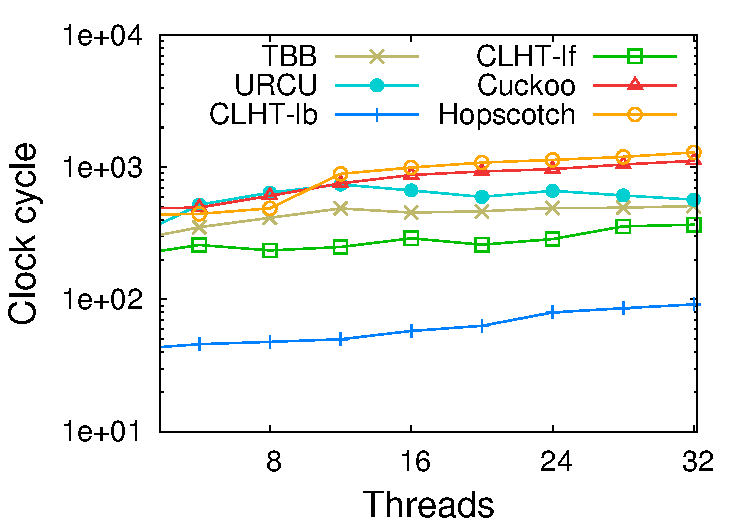
\includegraphics[width=0.45\textwidth]{getfail}}
\subfigure[get-suc]{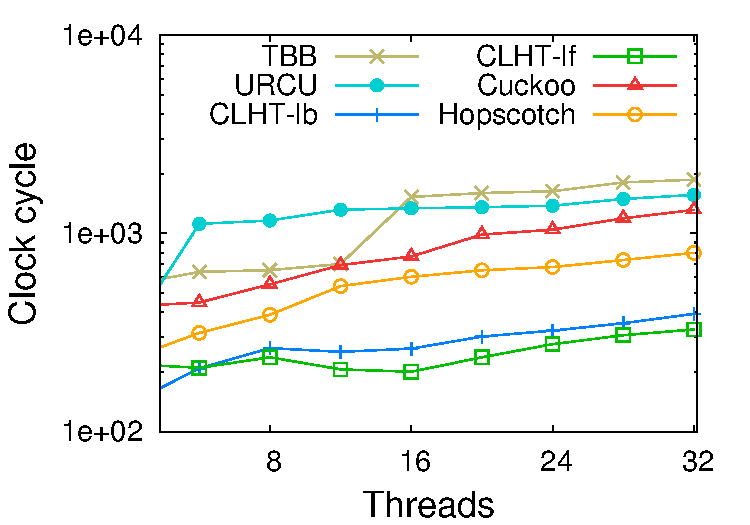
\includegraphics[width=0.45\textwidth]{getsuc}}
\subfigure[put-fail]{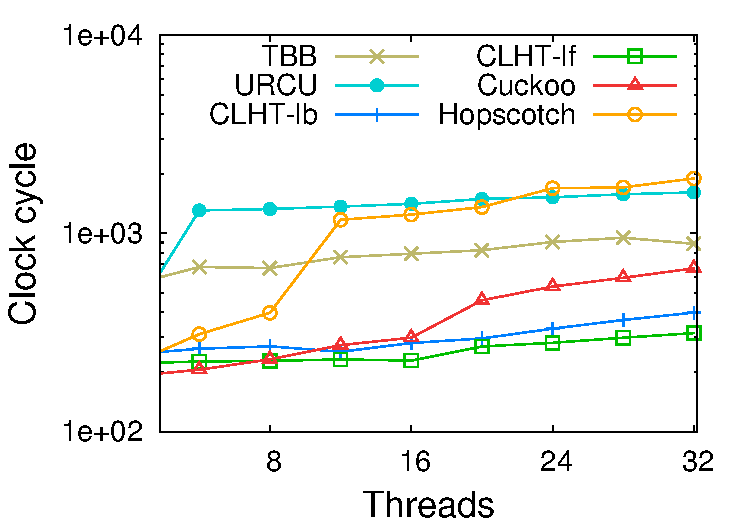
\includegraphics[width=0.45\textwidth]{putfail}}
\subfigure[put-suc]{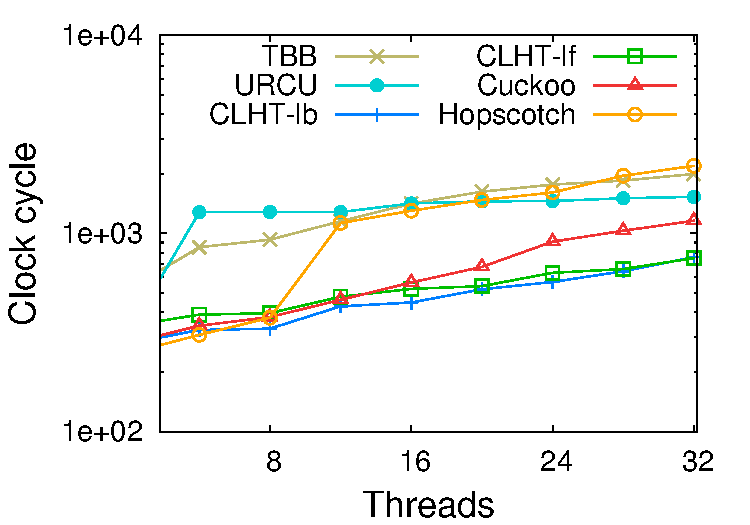
\includegraphics[width=0.45\textwidth]{putsuc}}
\subfigure[rem-fail]{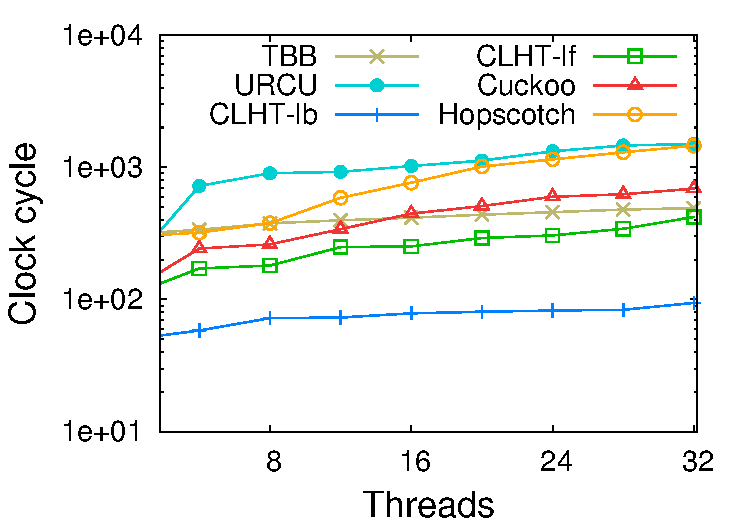
\includegraphics[width=0.45\textwidth]{remfail}}
\subfigure[rem-suc]{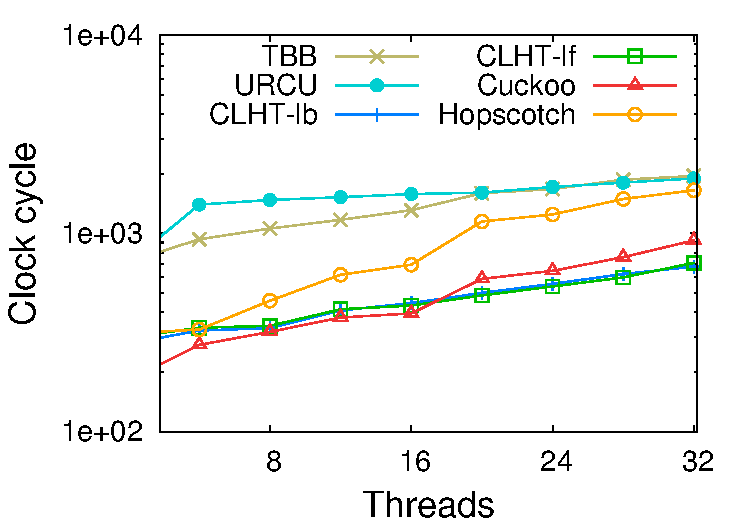
\includegraphics[width=0.45\textwidth]{remsuc}}
\caption{E5-2630平台上6种操作对应的延迟随线程数量变化曲线}
\label{fig:latency}
\end{figure}

Cuckoo从直观的计数器的数据来看它搜索操作耗费的平均时钟周期比更新操作的更高。
出现这种现象的原因是Cuckoo需要频繁的从较长的cuckoo路径中搜索元素。
在并发度较低的情况下,Cuckoo处理put-fail和rem-suc两种操作的延迟较低。
同样在线程数低于6的情况下,Hopscotch处理put-suc操作的延迟较低。TBB在处理fail类型的操作时的延迟相对稳定,但是在处理suc类型操作时与URCU持平,甚至在某些情况下比URCU表现更糟糕。

\textbf{分析:} David等人在其研究中提出的异步并发(ASCY)模式有助于获得良好的扩展性~\cite{clht}。
这一点在CLHT上得到很好的体现。
在实际应用中,ASCY的特定模式能够帮助开发人员在实现并发哈希表时避开潜在的陷阱。
比如,在对Hopscotch进行分析时,我们发现其在进行删除操作时对共享变量所做的修改,以及在更新操作的解析阶段的等待都与ASCY的原则相悖。
将删除操作替换成其它类型的操作进行测试发现其吞吐量有明显的增加。

\subsection{线程绑定方案的影响}
\label{sec:thread_pinning}
在多核计算机系统上线程到核之间的映射关系称为线程绑定。
线程绑定对于并发编程至关重要~\cite{pinning}。
在这一部分内容中,将以E5-2630为例,探究3种不同的线程绑定方案在4个多核系统上的表现有何区别。
图~\ref{fig:2630topology}所示为E5-2630平台上使用平衡型线程绑定方案时线程与核的映射拓扑结构。
该拓扑结构使用开源工具\textit{likwid}\cite{likwid}的\textit{likwid-topology}得到。
该平台具有两个socket,每个socket集成了八个物理核,每个物理核最多支持两个硬件线程。

\begin{figure}[htbp]
\centering
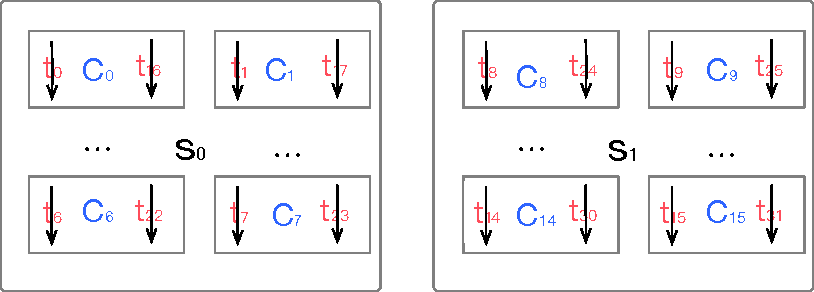
\includegraphics[width=0.6\textwidth]{2630topology}
\caption{E5-2630平台上使用平衡型线程绑定方案时线程与核的映射拓扑结构}
\label{fig:2630topology}
\end{figure}

在进行实验分析前,首先简要介绍实验中用到的三种不同方案:默认绑定方式和显示绑定方式,其中显示绑定方式又分为紧凑型绑定和平衡型绑定两种。

\textbf{默认方式}:线程通过系统调度器自动分配核。
操作系统调度器尽可能的实现多个核之间的负载均衡。这种绑定策略的好处是允许线程在执行过程中在不同的核之间迁移。

\textbf{紧凑型}:尽可能的将连续的线程映射到在拓扑结构上距离最近的核上。
如果需要创建24个线程,根据紧凑型绑定策略首先将第一个插槽内的核映射满,即就是线程t$_0$到t$_{15}$被映射到s$_0$内的c$_0$到c$_7$上,然后余下的线程将映射到位于s$_1$上的c$_8$到c$_{11}$上。
这种绑定方式的好处是在线程间提供较高的数据重用率。

\textbf{平衡型}:紧凑型线程绑定方案具有在单个插槽内共享缓存的优势,它的劣势在于紧凑型的线程绑定容易引起负载不均衡。
因此,平衡型绑定策略将线程均衡的绑定到位于不同socket的核上。
下面用一个实验测试中的实例进行说明:假设运行某次测试需要创建16个线程参与运算,正好可以将16个线程分别映射到c$_0$到c$_{15}$;
如果需要创建的线程数量超过了系统核的数量,这时才会启用超线程。使用平衡型绑定策略的好处有两方面:一是保持负载均衡;二是,在创建的线程数量少于系统具有的物理核的数量时,可以避免启用超线程产生的干扰。


\begin{figure}[htbp]
\centering
%\subfigure[Intel]{
\subfigure{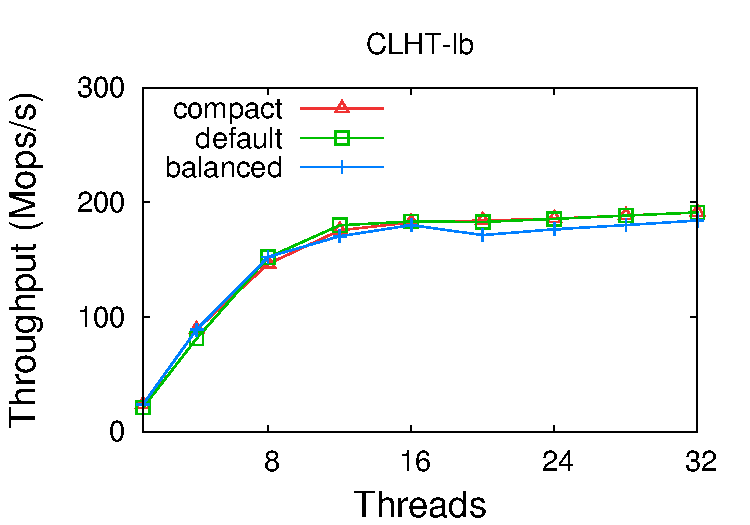
\includegraphics[width=0.3\textwidth]{2630clht}}
\subfigure{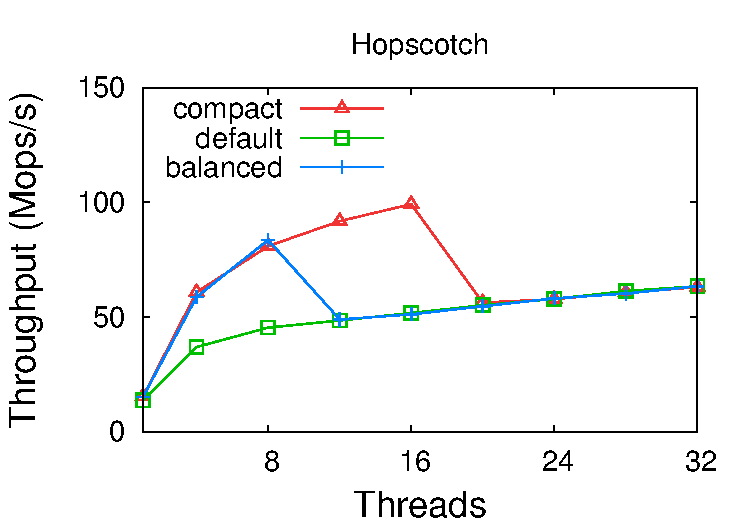
\includegraphics[width=0.3\textwidth]{2630hop}}
\subfigure{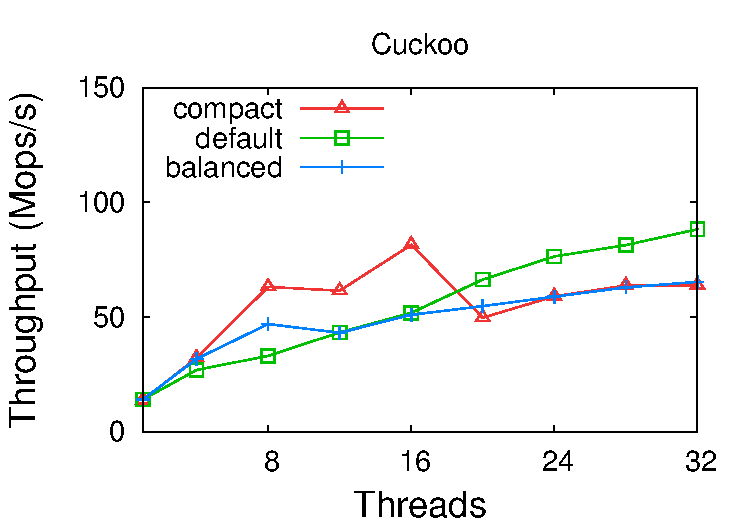
\includegraphics[width=0.3\textwidth]{2630cuckoo}}
\subfigure{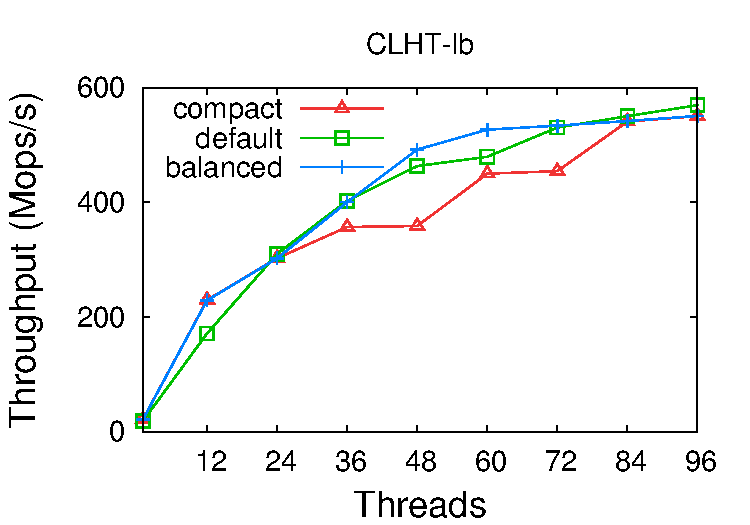
\includegraphics[width=0.3\textwidth]{4850clht}}
\subfigure{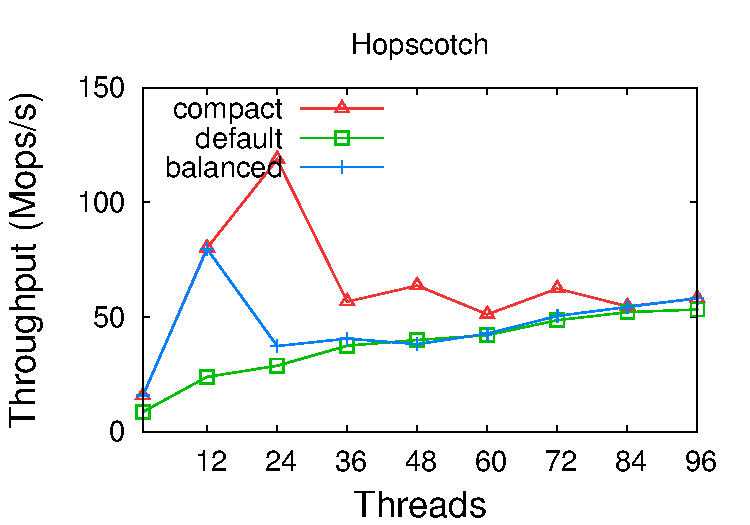
\includegraphics[width=0.3\textwidth]{4850hop}}
\subfigure{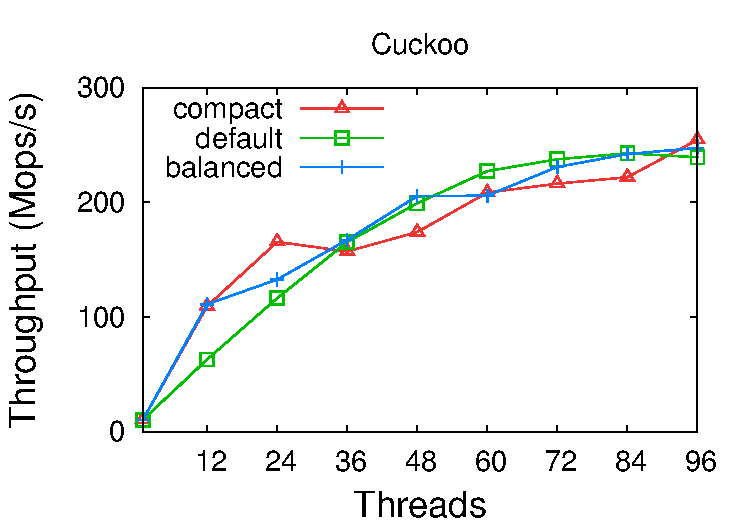
\includegraphics[width=0.3\textwidth]{4850cuckoo}}
\subfigure{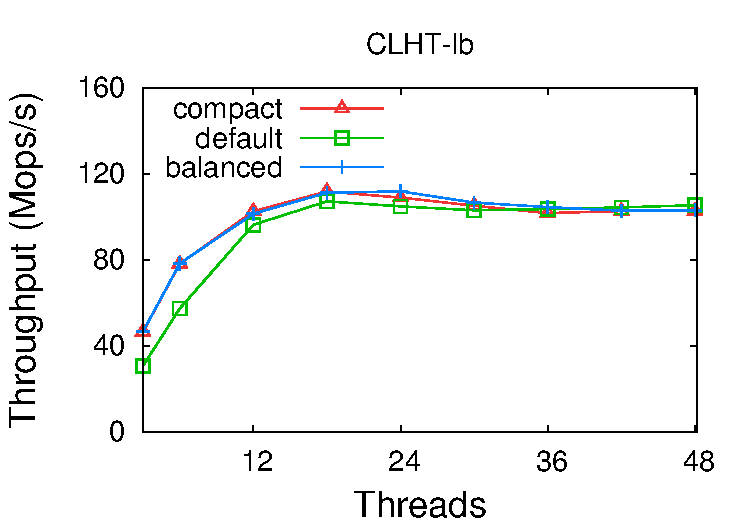
\includegraphics[width=0.3\textwidth]{AMDclht}}
\subfigure{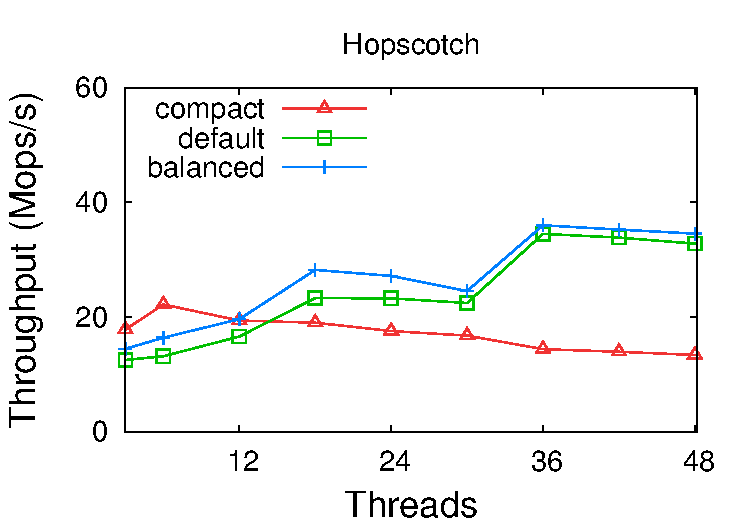
\includegraphics[width=0.3\textwidth]{AMDhop}}
\subfigure{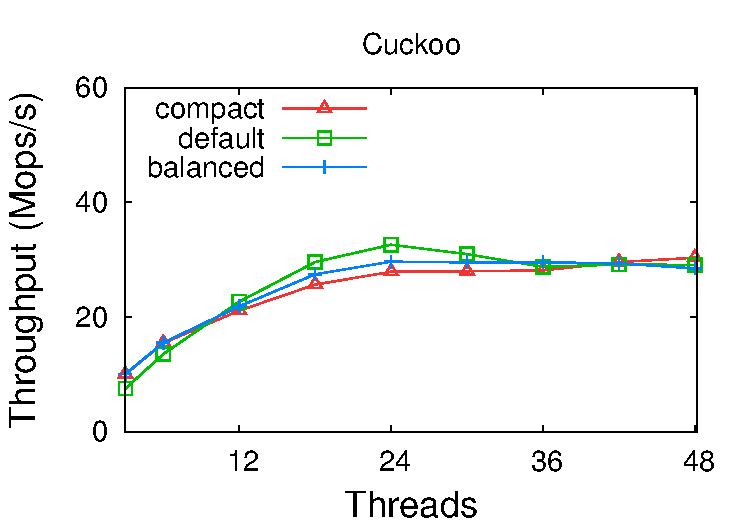
\includegraphics[width=0.3\textwidth]{AMDcuckoo}}
\subfigure{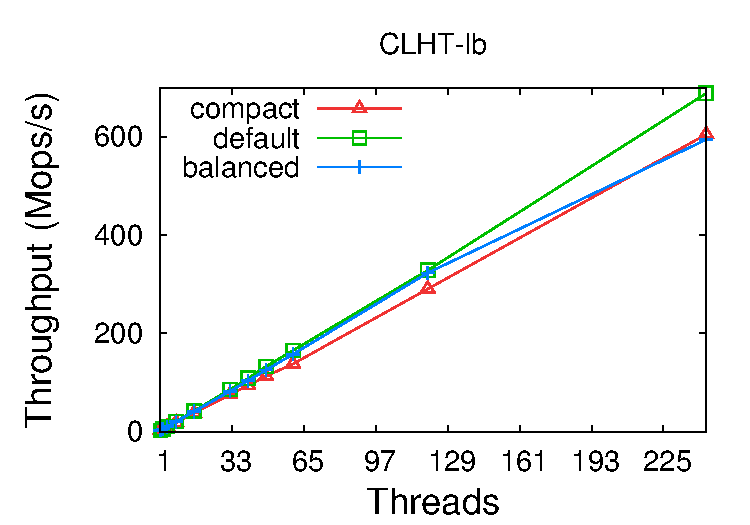
\includegraphics[width=0.3\textwidth]{7120Pclht}}
\subfigure{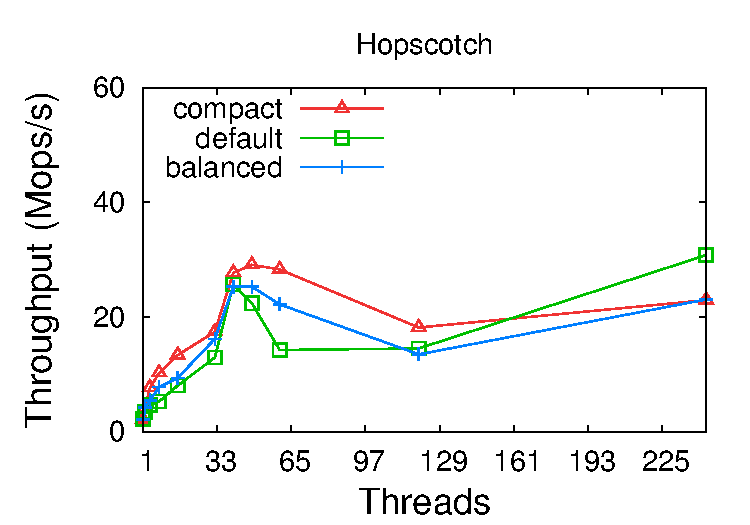
\includegraphics[width=0.3\textwidth]{7120Phop}}
\subfigure{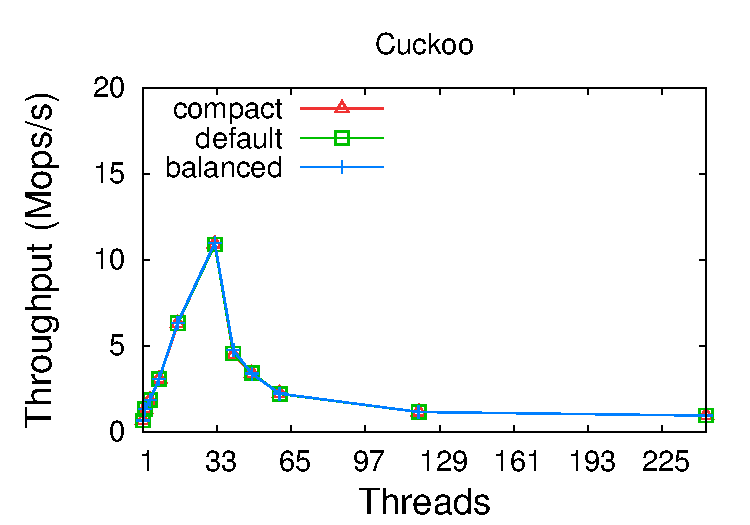
\includegraphics[width=0.3\textwidth]{7120Pcuckoo}}
\caption{三种线程绑定方式性能对比}
\label{fig:pin}
\end{figure}

CLHT的吞吐量受线程绑定方式影响较小,但Hopscotch和Cuckoo的吞吐量的波动却很大。
具体的以E5-2630为例,在该平台上以默认方式的性能曲线为基准,线程数量为8时,使用紧凑型和平衡型绑定策略性能提升了大约一倍。
进一步分析,在紧凑型线程绑定策略下,线程数达到16时,吞吐量比采用默认绑定方式提升了2倍。在E7-4850机器上体现了相同的趋势,故不再单独分析。

Hopscotch吞吐量显著的加速比来自于它的静态内存分配机制。
它在创建哈希表的同时就已经预先进行了内存分配,受Linux内核first 
touch内存分配策略的控制,预先分配的后果是导致所分配到的内存全部位于同一个NUMA结点上。所以,我们使用libnuma对其它并发哈希表进行优化,使其在进行动态内存分配时均衡的兼顾所有NUMA架构下的内存结点。
然而,当线程数从16向20变化(E5-2630),从24向36变化(E7-4850)过程中,吞吐量猛然下跌,这说明跨socket开销对性能的影响远大于此阶段参与运算的线程数量的增加。

而在AMD平台上,各哈希表的性能表现得对于线程绑定方式不敏感,这个现象可以从两个方面进行解释。
首先,Intel Xeon最后一级缓存的可包容性提供了较强的局部性,这种局部性提高了socket内通信的效率。
其次,在执行状态为’O’和’S’的缓存行上执行存储操作时,即便是所有的共享线程全部位于同一个socket内,AMD Opteron的不完整目录协议也会是跨socket间的流量失效。
因此,socket内的性能与跨socket情况下的性能基本一致。
由于负载的均衡分布使得该平台对跨socket通信不敏感,所以当线程分布在多个socket上时,默认绑定方法和平衡型绑定方法的性能要优于紧凑型绑定方式。

在Phi 7120P平台上,CLHT无论采用哪种绑定方式,性能都一如既往的好(吞吐量随着所创线程数量的增加呈线性增长)。
而Cuckoo采用三种不同绑定方式所获得的吞吐量不存在显著差别(三条性能曲线基本重合)。
这一点与之前在其它三个NUMA平台上观察到的结果存在较大差别,在NUMA平台上Cuckoo采用默认绑定方式具有最佳性能。
当线程数在[1,150]这个区间变动时,Hopscotch在Phi平台上使用紧凑型绑定策略获得最佳性能。
然而,在线程数超过150个之后,CLHT 和Hopscotch在这个阶段使用默认绑定策略的性能要优于其它两种策略。使用显示线程绑定策略的缺点是:受到二级缓存容量的限制,会造成更多的缓存未命中数量和过高的内存访问延迟。而在Xeon Phi上,默认绑定方式由于依赖于操作系统的调度器进行线程绑定并且允许线程在不同的核之间进行动态迁移,能够有效的降低资源竞争率并且更好的利用缓存子系统。
另外,Xeon Phi的表现类似与对成多处理机(SMP)系统,所有核到主存储器之间的距离是相等的。
将线程分配在不同的物理核上引起的开销与类似于NUMA系统上跨插槽的开销,但由于Phi上快速双向环状互联通道的设计使得跨核开销要远小于跨插槽开销。

\textbf{分析:} 通过实验表明没有哪一种绑定策略能在所测试的多个硬件平台上具有压倒性优势,也没有哪一种策略能够让所有的并发哈希表发挥最佳性能,所以在比较三种不同的线程绑定方案过程中没有一个统一的结论。
比如,在Intel Phi平台上,CLHT使用默认绑定方式具有最佳性能,但是在其它平台上则是其它绑定方式下具有最佳性能。
再就是Cuckoo在Phi平台上使用三种不同绑定方案的性能相当接近,没有哪一种具有明显的优势。因此,要探究并发哈希表的异常表现,需要结合并发哈希表的设计模式,线程绑定方案,创建的线程数量以及对应的硬件平台的特征进行考虑。
这对开发人员无疑是一种负担,最理想的解决方案是在运行过程中通过对硬件特征和工作负载的监控进行自适应的动态切换线程绑定策略,以达到获得最佳性能的目的。

\subsection{同步}
\label{sec:sync}
在并发读写的过程中,为了保障性能,多个线程对共享数据的访问需要用到同步方案对并发线程进行协调。
因此,设计并发哈希表时的另一个重要环节是同步方式的选取。
对线程间的同步处理不当会成为阻碍相关算法扩展性的最大障碍。
在这一部分中,将讨论并发哈希表中几种主要的同步机制以及运用不同的同步机制对性能会产生什么样的影响。

回顾图~\ref{fig:update}的性能曲线,几种并发哈希表中CLHT的性能最突出,尤其是在Phi 7120P平台上体现的最为明显。
CLHT获得突出线程扩展性的原因除了其在数据结构设计上的巧妙之处外,它所采用的同步机制的贡献也不容忽视。CLHT-lb使用原子快照对读者线程和写者线程进行同步。
具体的,在读者线程间,它使用由原子操作FAI(Fetch-and-Increment)实现的自旋锁对每个哈希桶进行保护。
采用这种方式的好处是,即便在并发度很高的情况下,竞争仍然保持一个较低的水平。
简单锁方法加上低竞争化合出理想的扩展性~\cite{david}。无锁的CLHT版本同样使用快照的方式进行同步,该快照的大小为8字节,它能在单个操作内被读取、存储或者CAS(Compare-and-Swap)。
在哈希桶内有一个版本计数器用于同步并发写线程,同时还有一张表示有效、失效或者正在被执行插入操作三种状态的位图。
以上就是CLHT获得卓越性能的原因。

在处理只包含读操作的工作负载时,发现Hopscotch的性能要优于CLHT。
而一旦工作负载中包含了更新操作,Hopscotch的性能有显著的下降。
并且这种下降幅度随着工作负载内更新操作比例的增加而增大。
这种现象也说明选取同步方案的重要性。Hopscotch使用TTAS锁对写线程进行协调。
写线程之间的同步开销要高于读线程间的开销。
为了减轻同步开销,在写线程和读线程之间使用时间戳。
Hopscotch在设计上特意使锁的数量等同于锁创建的线程的数量,这与CLHT相比无疑会引起更高的竞争。
更糟糕的是,Hopscotch使用的TTAS锁本身的扩展性也存在问题。以上对Hopscotch严重的性能下降现象就同步方面作出了解释。

Cuckoo的实现也是基于细粒度锁。
它使用锁对读-写和写-写两种访问模式进行同步。
Cuckoo使用的是条纹状自旋锁,锁的实现使用CAS(Compare-and-Swap)原语。
TBB使用细粒度锁对每个哈希桶进行保护,这一点与基于锁的CLHT的设计思想相似,但二者的区别是TBB每个哈希桶内包含的键/值对的数量要远多余CLHT。

如图~\ref{fig:thread_scal}(d)和图~\ref{fig:update}(d)所示,并发哈希表在Xeon Phi平台上性能曲线与其它三个NUMA平台存在明显差异。
Xeon Phi使用的是扩展的MESI缓存一致性协议,该协议用GOLS(Globally Owned Locally Shared)模拟共享状态以允许对处于修改状态的缓存行实现共享,对处于GOLS状态的缓存行进行存储同样会引起无效的通信。
过高的一致性流量很容易使Phi的环状互联通道达到饱和。
从实验结果可以推断,CLHT的设计同样很好的适用于Xeon Phi的体系架构。而Cuckoo在该同台上的性能很差,即便是处理只读的工作负载,其性能也不理想。
其原因在于每一次查询操作,与给定哈希值相关联的哈希桶都被上了锁,这严重的限制了并发度,从而影响了其在该平台上的性能。

\textbf{分析:} 同步在并发哈希表的性能中扮演者至关重要的角色。
然而,并不存在一种放之四海兼准的通用的同步方案,设计一种高效的同步机制需要综合考虑来自底层原语到体系结构特征再到高层锁实现乃至并发模型的影响。
正如我们通过实验分析的那样在MiC架构平台上,除了CLHT之外,其它并发哈希表反常的性能地下表明获得可移植的高性能任重道远。
在实践当中,判断同步机制是否合适,需要全面的理解上述因素的多方面影响。
例如,在设计锁算法时,需要知道在特定的平台上怎样选择更合适的原子原语,而这又取决于缓存一致性,以获得更好的性能。
更进一步说,有些锁在高竞争环境下表现良好,而有些锁在低竞争情形下更具有竞争力。
因此,实现自适应锁来利用不同锁算法的优点将是一项有价值的研究工作。

\subsection{内存消耗}
\label{sec:memory_comsume}
在物理内存有限的场景下,对于CHT这种内存密集型应用而言,除了对于性能方面的需求之外,另一个重要的指标是内存的消耗。
在运行时间一定的情况下,获得相同的吞吐量所消耗的内存越小,该应用就越占据优势。
下面对四种动态分配内存的并发哈希表的内存使用情况进行分析。

表~\ref{tab:memusage}~给出各个并发哈希表使用16个线程运行含有10\%更新操作的不同初始化元素个数的工作集时的内存使用情况。单位为MiB。
内存使用情况使用Linux系统的系统监测工具测量。
在初始化元素值相同的前提下,Cuckoo在处理规模叫大的工作集时内存效率更高,URCU仅次于Cuckoo,并且处理小规模数据集时具有更高的内存效率。CLHT和TBB在同等规模数据集下所消耗的内存时Cuckoo和URCU的几倍。


\begin{table}[htbp]
  \centering
  \caption{E5-2630平台上的内存使用情况}
  \label{tab:memusage}
  \begin{tabular}{cccccccc}
    \toprule
       \textit{i}   &   TBB   &    CLHT    &  URCU     &  Cuckoo &     Hopscotch \\
    \midrule
$10^3$     & 0.6  &   1   &  \textbf{0.6}   & 63 &   608.6    \\

$10^4$     & 2.2   &  15.4   &   \textbf{1.8}    & 63  &   608.6    \\

$10^5$     & 14.1 &    34.4   &   \textbf{7.8}   & 63  &  608.6     \\

$10^6$     & 80   &  78.4    &   \textbf{43.9}   & 101 &  608.6       \\

 $10^7$    &  857  &   1024   &   645    & \textbf{633} &  608.6     \\

 $10^8$    &  5.5 GiB  &   8 GiB   &   5 GiB    & \textbf{2.3} GiB &       \\
    \bottomrule
  \end{tabular}
\end{table}

产生这种差异的原因是什么呢?接下来的内容将对这个问题进行说明。

Cuckoo内存效率高的原因来自两个方面。
首先,Cuckoo组相联的设计节约了空间,提高了空间使用效率。
其次,使用版本计数器代替指针连接其它哈希桶,在处理键值对很小的条目时具有极高的内存效率。
CLHT和TBB都使用细粒度锁对每个哈希桶内的键值对进行保护。
这种机制的的好处是处理速度快,但是在处理大规模键值对的工作集时,指针将消耗大量的内存。
所以,使用细粒度锁机制是一种通过牺牲空间换取性能的优化方式。

\textbf{分析:} 一方面,相同配置下较低的内存开销的应用能够处理更大规模的工作集,并且降低了操作系统发生页切换的概率,降低页切换概率有利于降低来自平台对性能的影响。
另一方面,内存效率依赖于数据间的管理机制,而数据管理机制的选择也会在一定程度上对性能造成影响。
链式结构的并发哈希表需要额外的指针对哈希桶进行链接,尤其是以CLHT最为突出,它的哈希桶的容量被设计成与缓存行的大小一致,这就需要在每个缓存行都预留一个字节的指针以便与其它的哈希桶进行链接,而Cuckoo的组相联的设计减少了这种指针的使用,降低了额外的内存开销。
另外,锁的粒度越细,所消耗的内存空间也越多。
总而言之,对数据的组织结构和同步的粒度进行优化有助于提高性能,其代价是更高的内存开销。

\section{本章小结}
并发哈希表在现代多核软件系统中占据至关重要的地位。
为了解决特定硬件环境与错综复杂的算法设计中的实际问题,相关研究人员提出了一系列的并发哈希表的设计方法。
用户如果需要从众多的相关算法中选择一个适合自己应用的算法就需要深入透彻的去了解现有并发哈希表的优缺点。
然而,事实却是不同的并发哈希表要么是根据特定的应用软件设计的,要么是针对特定的硬件平台进行优化,缺乏统一的评测基准。
这对并发哈希表的设计、优化,并发哈希的应用都造成了不便。

基于上述考虑,首先设计一套用于测试评估并发哈希表的统一的测试框架(CHTBench),为并发哈希表的评估提供一个相对公平的环境,避开因工作负载、键值对生成方式等因素的干扰。
随后使用CHTBench对现有文献中影响力较高的5种并发哈希表进行测试评估。
评估和比较的指标辐射面从宏观的吞吐量到微观的延迟,从片上缓存到主存,从复杂的同步机制再到可移植优化等,并在每一项指标的评估之后做了针对性的分析。

本章对并发哈希表的比较和评估工作是迄今为止覆盖面最广,指标最多,最有深度的。
文中设计CHTBench和测试方法对并发哈希将来的设计研究和应用推广具有重要价值。 

% 
\chapter{基于硬件事务内存的并发哈希表的实现}

%备选标题:基于RTM的锁省略算法
\section{事务内存的基本概念}
事务内存(TM)是一种简化并发编程的并发控制范式,其源自于数据库管理系统中的事务概念。
它的核心思想是将一段代码标示成一条事务。
在数据库管理系统中,事务必须满足ACID性质,即原子性(Atomicity)、一致性(Consistency)、隔离性(Isolation)和持久性(Durability)。
原子性指的是事务中的动作要么全部执行,要么一个都不执行;一致性指的是任何时刻,数据库必须处于一致性状态,即必须满足某些预先设定的条件;隔离性是指一个事务不能看见其它未提交事务所涉及到的内部对象的状态;而持久性则是指一个已提交的事务对数据库系统的改变必须是永久的。

事务内存继承了事务的ACID原则。
事务内存的原子性是指事务代码区间的内容要么全部执行,要么全部不执行,不存在有事务代码停滞在中间的任何一条语句,如果发生意外而中止了事务,则系统状态会回滚到事务起始的状态继续执行;
事务内存的一致性是指是指事务应该要么执行完成并令外界看到其造成的变化,要么执行失败并使所有相关状态都保持不变。如果有多个事务同时运行,那么从这些事务之外的角度来进行观察,它们对系统状态做出的改变始终是一个接着一个发生的,中间不会有任何交叉。例如,在(对同一个账户)两个独立且并发的存款和取款事务完成之后,账户余额应该是两个操作所产生的累加效果(取钱是对账户加上一个负数)。
事务内存的隔离性是指并发执行的多个事务代码区间彼此之间是严格隔离的,本事务无法了解其他事务的局部变更结果,所有事物造成系统状态的变化只有在成功提交之后才对外部可见;
事务内存的持久性是指事务代码执行完成成功提交之后,对于系统状态的变更是持久有效的,并不会回退到起始状态,直到有新的事务执行的代码改变这个状态。

事务内存具有两个重要的性质,即事务内存要确保对临界区代码片段的执行具有原子性和隔离性。
满足原子性和隔离性的事务内存可以安全的并行执行,可以取代现有的令人头疼的锁机制与原子原语。
基于锁的并发编程是一种悲观的并发模式,它假设获得锁的线程一定会访问共享数据,从而会对其他线程进行阻塞。
而任意两条访问加锁的变量的事务能够并发的执行,并且只有在其中一条事务尝试修改共享数据时触发回滚。

事务内存被认为是最有希望解决多核处理器编程问题的并发编程方案之一。
它最吸引人的特点是程序员只需在本地对共享数据的访问进行推理,并让底层系统确保正确的并发执行。
该模型有望提供细粒度锁机制那样的线程扩展性并能避免由一般的锁机制中常见的陷阱,比如死锁等问题。

事务内存发展到今天,有两种实现方式,一是基于软件的事务内存(STM);一是基于硬件的事务内存(HTM)。
不论是软件事务内存\cite{spear2010lightweight,saha2006mcrt,shavit1997software}还是硬件事务内存\cite{yen2007logtm,moore2006logtm,dalessandro2011hybrid}都得到了充分的研究与长足的发展。
随着IBM z系列~\cite{Cain2013Robust}和p系列~\cite{Wang2012Evaluation}处理器以及Intel Haswell处理器~\cite{Intel2015Intel}的问世,标志着硬件事务内存~\cite{Herlihy1993Transactional}走向市场化。

本章主要研究硬件事务内存对构建并发哈希表的作用。

\section{Intel事务同步扩展}
2012年2月,Intel发布了其支持硬件事务内存的事务同步扩展(Transactional Synchronization Extensions, TSX),并于2013年6月在其基于Haswell微体系结构的微处理器上亮相。
标志着硬件事务内存的全面商用化。

TSX对使用锁锁省音方式编写的多线程并发软件具有明显的加速所用。 
TSX提供一组扩展指令集,允许编程人员指定事务同步的代码区域。
有了事务同步,硬件就能动态的决定线程是否需要对锁保护的临界区进行串行化,并且只在必要的时候执行串行化。
这允许处理器利用由于动态的不必要的同步而隐藏起来的并发性。
在Intel TSX的最底层,编程人员指定的代码区域(也称为事务区域)就能事务性的执行。
如果事务执行成功完成,那么对其他逻辑核而言所有在事务区间执行的内存操作都像是在瞬间发生的。
只有确认成功提交后,在执行事务区域期间对于系统的更新操作才会对其他逻辑核可见,该过程称为一次原子提交。
这样,编程人员只需使用粗粒度的锁编程就能实现细粒度锁的性能。
如果多个线程同时访问受同一个锁保护的临界区而彼此之间有不存在任何数据冲突,那么这些线程就能并发的执行而无需串行化。

Intel TSX提供两种不同的软件接口。一种称为硬件锁省略,Hardware Lock Elision (HLE);一种称为限制性事务内存,Restricted Transactional Memory (RTM)。

\subsection{Intel硬件锁省略}
HLE提供与传统指令集兼容的指令集接口供编程人员编写事务化的程序,还提供两条全新的指令前缀XACQUIRE和XRELEASE。

使用HLE时,将XACQUIRE前缀放置在用于获取保护临界区的锁的指令的前面。
处理器将XACQUIRE视为省略写相关的锁获取操作的提示。
即使是获取锁的请求与该锁有关联的写操作,处理器也不会将锁的地址添加到事务区域的写集中而是将锁的地址添加到事务区域的读取集中,更不会向该锁发起任何写入请求。
之后逻辑处理器进入事务执行。
如果在XACQUIRE前缀指令之前是可用的,那么后面的其他所有的处理器都将该锁视作是可用的。
因为当前正在事务化执行的逻辑处理器不会将锁的地址写入到它的写集中,也不对其执行外部可见的写操作,其他的逻辑处理器仍然可以读取该锁而不会造成数据冲突。
这就允许其他的逻辑处理器也进入并且并发的对受同一个锁保护的临界区进行操作。
处理器将自动检测事务执行期间发生的任何数据冲突,有必要时执行中止事务操作。

XRELEASE前缀放置在用于释放保护临界区的锁的指令的前面。这涉及到对锁的写的问题。
如果XRELEASE正在试图将锁的值恢复到XACQUIRE发起锁请求时所操作的同一个锁的值,那么处理器将省略所有与即将释放的锁相关的所有外部锁请求并且该锁的地址不会被添加到写集中。
然后处理器尝试提交事务执行。

使用HLE时,有多个线程同时执行到被同一个锁保护的临界区时,如果它们执行的操作不会相互之间产生数据冲突的话,这些线程可以并发执行。
如果无法事务的执行代码区域,处理器将不使用省略而以普通的方式执行代码区域。
HLE确保软件有与基于锁的非HLE模式相同的前向执行的能力。
对于一次成功的HLE执行,锁和临界区代码都必须遵循特定的指导原则~\cite{Intel2015Intel}。
这些指导原则将会对性能产生影响,不遵循这些指导原则不会造成功能性的失败。

不支持HLE的硬件会忽略掉XACQUIRE和XRELEASE前缀提示,也不会执行任何省略操作。
更为重要的是,HLE很好的与现有的基于锁的编程模型兼容。
在基于锁的编程模型中不正确的使用XACQUIRE和XRELEASE前缀提示不会引起功能错误,但它可能会暴露代码中已经存在的潜在的漏洞。

\subsection{Intel限制性事务内存}
RTM为事务的执行提供了更为灵活的接口。
它提供三条新的指令——XBEGIN, XEND和XABORT——供用户启动,提交和中止一次事务执行。

XBEGIN指令用于指定事务代码区域的起始位置,XEND指令表示事务代码区域的结束。
XBEGIN指令携带一个操作数,该操作数用于表示到回滚指令地址的相对偏移量,如果RTM代码区域无法成功的进行事务化执行,将会推到该操作数指向的指令继续执行。

处理器有很多原因中止RTM的事务执行。
硬件自动检测事务中止条件,退回到回滚指令处以从XBEGIN开始的指令时的体系结构状态和EAX寄存器更新的描述事务中止的状态重新开始执行。

XABORT指令允许用户显示的中止RTM代码区域的执行。
它携带一个8位的直接参数,这个参数被加载到EAX寄存器中并将在发生RTM中止后对软件可见。具体参数的意义见表~\ref{tab:rtm_status}~。

\begin{table}[htbp]
  \centering
  \caption{RTM的中止状态定义}
  \label{tab:rtm_status}
  \begin{tabular}{cc}
    \toprule
       EAX寄存器比特位 & 说明 \\
    \midrule
      0     & 由XABORT指令引起的中止 \\
      1     & 该事务有可能在Retry之后成功\\
      2     & 该次中止是因数据冲突而引起的 \\
      3     & 该次中止是因内部的缓存溢出引起的\\
      4     & 该次中止是因调试断点引起的 \\
      5     & 该次中止是因事务嵌套引起的 \\
      23:6  & 保留位\\
      31:24 & XABORT参数(只有位0被置位时有效) \\
    \bottomrule
  \end{tabular}
\end{table}

RTM指令没有任何与它们相关联的数据存储位置。
虽然硬件无法保证RTM区域总是能够成功地进行事务地提交,但大多数遵循推荐指南的事务都有望成功地进行事务处理。
然后,用户必须在回退路径中提供备选的代码序列,以确保程序的前向执行。
比如,通过简单的锁申请然后以非事务的方式执行制定的代码区域。
此外,总是在特定的实现中发生中止的事务可能会在接下来的实现中完全事务的执行。
因此,用户必须确保事务性区域代码的路径和备选代码序列在功能上是完备的。

使用Intel RTM必须获得相应的硬件支持,在不支持RTM的平台上无法完成编译。
这是RTM有别于HLE的地方之一。

\subsection{TSX的Lemming效应}
\textit{Lemming}效应是指正在运行中的事务之间陷入一种相互阻扰对让进入事务执行的状态。
具体的,任意获得锁的线程会对锁变量进行修改同时强制其他当前正在该锁上执行锁省略过程的线程中止。
这些被中止的线程随后会尝试重新尝试事务的执行或者尝试获取锁。
当存在多个线程都处于这一过程时,这些线程会陷入一种持续阻挠对方回退到回退路径的状态,使得锁省略过程长时间停滞。

被省略的锁有一个强制的惯例,即要么所有的锁用户都是省略的,要么所有的锁用户都是真实的持有锁。
一般的情况下总是这样,除了一些特殊的情况可以避免这种惯例。
这种惯例确保对任何实际持有锁的线程执行正确的锁语义。

在HLE中,受锁保护的代码段执行时通过启动一条事务并假装“获取”锁但实际上并没有真正持有该锁。
也就是说,锁被读取,如果它的状态被解锁,那么它就被放置在被锁住的事务读集中,而不影响锁的状态,这仍然保持解锁状态。
然而,当事务中止时(例如发生冲突),它会执行回滚然后以非推测性的方式获取锁,并将锁写入。
被中止的线程获取的全局可见的锁与执行推测运行的HLE事务时推测性加载的锁发生冲突,由于在锁的位置上发生了冲突,所以会导致所有这些锁被中止。此外,当新的线程到达临界区时发现当前锁已经被其他线程持有时,新的线程不会启动它们的事务。
在公平锁的情况下,获取锁时的冲突会使得线程无法并行的执行,这种情况一直会持续到经历一个没有线程试图访问锁的静默期为止。
这种引起不必要的串行化从而限制并发度的现象称为\textit{Lemming}效应~\cite{Dice2008Applications}。

当中止率升高时,\textit{Lemming}效应的影响会越来越严重。
如果是在中止率很低的情况下,\textit{Lemming}效应的影响可以忽略不计。
从本质上说,\textit{Lemming}效应使得事务从中止中恢复过来的成本更高,并且引起不必要的序列化执行。

在事务的执行过程中,常常由于冲突而导致事务中止。
事务申请获取的锁当前被其他线程占有从而被迫中止,但是占有该锁的线程可能很快执行完成并释放锁。
因此,大部分被中止的事务经过一次或者多次重试之后可以成功获取锁,完成提交。
Intel在TSX开发者手册中提倡使用RTM进行锁省略编程时适当的进行RTM重试有助于提升性能。
使用RTM编写锁省略代码时,如下行为会引起\textit{Lemming}效应的加剧:

\textbf{第一,过快的进行RTM重试。}当检测到发生中止时立即进行重试。
考虑这么一种情况,设定最大重试次数为5次(重试5次仍然无法成功提交则方式事务执行转而使用常规方式申请锁执行),假设现在有t$_1$和t$_2$两个线程在并行的执行事务代码,t$_1$长时间的持有锁。
这时t$_2$尝试申请锁,但发现当前锁不空闲,于是立即开始重试,重试次数很快达到5次,此时t$_1$仍然没有释放锁,t$_2$回滚,然后使用标准方式申请锁完成执行。
如果有更多的线程并行的处于上述状态,它们将陷入\textit{Lemming}效应的魔咒。
这些重试达到最大次数进入回滚路径执行的线程排队等待锁执行,长时间无法再一次进入到事务执行。
对性能造成损耗。

\textbf{第二,设定的RTM重试次数过大。}一般的,在使用RTM进行锁省略编程时通常能够提升性能。
而且,对于不同的工作负载最大重试次数是弹性变化的。
但是,当设定的重试次数过大时,会有加剧运行其他工作负载的\textit{Lemming}效应的风险。
同样以t$_1$和t$_2$为例,假设t$_1$和t$_2$都尝试事务执行,它们运行临界区,一定的时间后同时造成对方中止。
然后,它们进行重试,又一次遇到上述情况,如此循环若干次。
摆脱这种纠缠不清的状态的方法是其中一方进去到回退路径申请标准锁执行。
但是,如果重试次数过高,它们在进入回退路径之前会浪费较长的时间。

\textbf{第三,不设定回退路径,不停的进行重试。}除了冲突可能造成事务中止之外,还有其他原因(比如执行TSX不兼容的指令,动态连接库,页脏位以及其他异常等)也会造成中止,TSX不能保证每次事务执行都能成功。
不设置回退路径可能导致程序挂起。

\textbf{第四,没有将锁变量放入读集合内。}锁省音依赖于其读集合中的锁变量,用来确保推测行执行和真实的锁持有者之间的完全同步。
这要求在事务执行过程中至少读取一次锁变量。
如果该锁只使用单一的锁变量,那这个过程将由HLE自动完成,但是当锁有多个锁变量的时候,即便是有HLE的的情况下,这个过程也可能会出错。

\textbf{第五,在事务执行完成时使用\textit{xtest}代替锁的状态检测。}

\section{软件优化的硬件锁省略技术}

在使用硬件事务内存设计并发哈希表时,为了减轻
\textit{Lemming}效应对性能造成的负面影响,Intel的开发者手册中建议对被中止的事务进行重试~\cite{Intel2015Intel}。
然而,从上一节中关于触发\textit{Lemming}效应的原因中得知,过快、过度的使用RTM重试或者不对RTM重试的次数做出限定同样会引起\textit{Lemming}效应。
Y. Afek等人通过实验也表明这种简单的技术方案并没有完全缓解这个问题~\cite{Afek2014Software},尤其是当\textit{Lemming}效应很严重时,比如使用公平锁或者高并发度情况下,单纯的依靠使用RTM重试不能有效缓解\textit{Lemming}效应的副作用。
为了有效的抑制\textit{Lemming}效应造成的性能下降问题,他们提出了两种软件辅助的优化方案:软件优化的硬件锁删除方法和软件辅助的冲突检测方法。

\subsection{软件辅助的硬件锁删除方法}
软件辅助的锁删除技术,Software-assisted lock removal (SLR),是为了克服Lemming效应的影响,引入的第一种方法。
这种方法可以视为对Rajwar和Goodman~\cite{Rajwar2002Transactional}硬件锁删除技术的软硬件混合实现。
Rajwar和Goodman观察到只要事务内存能够为冲突的事务提供前向保证,那么就可以不需要锁执行具有相同临界区的事务(也就是通过启动事务代替申请锁,提交事务代替释放锁)。
然而,Haswell的硬件事务内存使用非常简单的“请求者至上”的冲突解决策略~\cite{2011Intel},而这一策略容易引起“活锁”~\cite{Bobba2007Performance}。

\SetKwProg{Fn}{Function}{}{}
\begin{algorithm}[htbp]
\SetAlgoLined
\Fn{lock()}{
  $retries \gets $ 0 ~~\\
  // speculative path~~\\
  XBEGIN (line 6)   \tcc*[f]{如果发生中止,跳转到第6行重试}\; 
  \Return
  ~~\\
  // fallback path~~\\
  $retries \gets retries + $ 1 ~~\\
  \eIf{$retries < MAX\_RETRIES $}{
    goto Line 3
  }{
    lock.lock() \tcc*[f]{执行标准锁请求}
  }
}
\caption{SLR的加锁方法}
\label{algo:slr_lock}
\end{algorithm}

SLR方案使用如下方法避免上述提到的问题,其加锁和解锁过程如算法~\ref{algo:slr_lock}~和~\ref{algo:slr_unlock}~所示。
在算法~\ref{algo:slr_lock}~中,第3行标示事务代码区域的起始位置,如果发生中止,则跳转到第6行尝试再一次的以事务的方式执行,如果重试的次数超过预先限定的门限值MAX\_RETRIES,则放弃事务执行,转而用普通的方式通过申请锁完成本次执行(第10行)。

\SetKwProg{Fn}{Function}{}{}
\begin{algorithm}[htbp]
\SetAlgoLined
\Fn{unlock()}{
   \eIf{$ XTEST() $}{ \tcc*[f]{如果本次为事务执行,返回TURE}~~\\
      \eIf{lock is $ TRUE $}{
          XABORT       \tcc*[f]{中止事务执行}
      }{
          XEND
      }
   }{
      lock.unlock()   \tcc*[f]{以标准解锁方式解锁}
   }
}
\caption{SLR的解锁方法}
\label{algo:slr_unlock}
\end{algorithm}

SLR使用HTM在不访问锁的情况下事务的执行临界区,直到准备提交。
如果当前锁未被其他线程持有,则SLR读取锁并提交;否则的话发生事务中止并重试。
重试多次之后仍然失败,此时SLR会放弃事务的执行转而以非事务的(常规的)方式申请锁完成该次操作。
在SLR中,获取锁的线程不会自动与运行事务冲突,也不会阻止到达的线程以推测的方式启动事务。
因为在SLR中,推测的事务可能并发的运行到持有锁的事务中,此时推测事务可能看到不一致的状态(这将确保推测事务提交失败然后中止)。

\subsection{软件辅助的冲突检测方法}

算法~\ref{algo:scm_lock}~和~\ref{algo:scm_unlock}~描述了SCM的加锁和解锁的过程。

\SetKwProg{Fn}{Function}{}{}
\begin{algorithm}[htbp]
\SetAlgoLined
\Fn{lock()}{
  $retries \gets 0$ \; 
  \tcc{primary path}~~\\
  XBEGIN (line 6)   \tcc*[f]{如果发生中止,跳转到第6行重试} ~~\\
  条件成熟时调用HLE或者SLR的$lock()$方法\;
  \Return
  ~~\\

  \tcc{serializing path}~~\\
  \eIf{aux\_lock\_owner  is $ FALSE $}{
      $ retries \gets retries + $1\;
  }{
      aux\_lock.lock()      \tcc*[f]{辅助锁申请锁}~~\\
      $aux\_lock\_owner \gets TURE$
  }
  \eIf{ $retries < MAX\_RETRIES $}{
      goto Line 3
  }{
      main\_lock.lock()
  }
  }
\caption{SCM的加锁方法}
\label{algo:scm_lock}
\end{algorithm}

软件辅助冲突管理技术(Software-assisted Conflict Management, SCM)。
SLR方法虽然能够很好的抑制\textit{Lemming}效应,但是以损失不透明度为代价。
SCM是另一种抑制\textit{Lemming}效应的软件辅助方法。
SCM是一种简单的冲突管理技术,它允许不冲突的线程继续运行其推测性的基于HLE的事务,而不受产生冲突的线程的影响。
为此,在锁的实现中添加一个串行化的路径,其中一个被中止的线程必须获得一个独立的辅助锁(不使用锁省略)以便重新加入与其他线程的推测执行。使用这种方法,发生冲突的线程之间被串行化,而不影响其他线程的并行执行。
如果线程在多次冲突中失败,那么它必须放弃推测执行转而申请原始锁。


SCM方法使用了两种锁,一种为主锁(\textit{main\_lock}),一种为辅助锁(\textit{aux\_lock})。
主锁使用的是HLE/SLR机制中的一种,而辅助锁是一种标准的传统锁。
只有在以标准的非事务执行方式执行代码区域时才会申请使用辅助锁(算法~\ref{algo:scm_lock}~第9、10行)。
辅助锁会将所有陷入冲突的线程召集到一起,然后将它们串行化的执行。
当某一事务被中止时,被中止的线程以非事务性的方式申请辅助锁,随后重新加入到对原始临界区的推测执行队列中。
这种为了重新加入到推测执行队列而申请辅助锁的过程称为串行化的路径(serializing path)。
线程在进入串行化路径之前会对事务进行重试。

\SetKwProg{Fn}{Function}{}{}
\begin{algorithm}[htbp]
\Fn{unlock()}{
\eIf{XTEST()}{
  调用HLE或者SLR的$unlock()$方法
  XEND
}{
  main\_lock.unlock()
}
\If{$ aux\_lock\_owner = TRUE $}{
  aux\_lock.unlock() ~~\\
  $aux\_lock\_owner \gets FALSE$
}
}
\caption{SCM的解锁方法}
\label{algo:scm_unlock}
\end{algorithm}
SCM和SLR也可以结合起来进一步减少当SLR线程放弃并以非事务的方式申请锁时引起的任何前向问题。

上述的两种软件辅助方法已经使用标准的pthread锁接口封装到动态库中。
可以直接在程序中使用上述方法而无需对代码进行调整,也无需重新编译。


\section{基于HTM的并发哈希表的设计}

\subsection{问题引入}

%哈希表操作示意图
\begin{figure}[htbp]
\centering
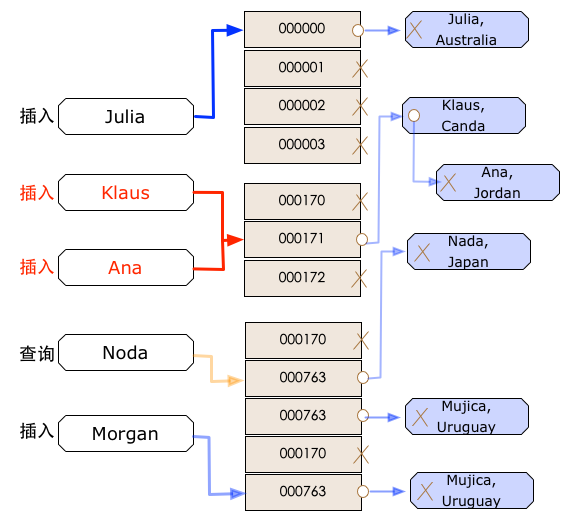
\includegraphics[width=0.9\textwidth]{hashtable}
\caption{串行执行五个操作的哈希表}\label{fig:hashtable}
\end{figure}

哈希表用于在线性时间内对键和键值对之间建立映射关系。
插入和查询是哈希表的两种核心操作,当然哈希表的扩张和删除操作也很重要,但是这里为了简要的引出我所要解决的问题,暂时不考虑哈希表的扩张和删除操作。

考虑这么一种场景,有一个简单的如图~\ref{fig:hashtable}所示哈希表,它串行的执行五次操作,分别是插入、插入、插入、查询、插入。
现在变更需求,希望将这个哈希表设计成并发的,会有怎样的问题呢?

设计高并发的哈希表并不是一件简单的事,目前有很多方法,比如基于锁的方法,使用原子指令实现的无锁化编程等,用于构建高并发度的并发哈希表。
但是这些方法无疑都会涉及到更加复杂的数据结构的设计,同时也增加了程序的复杂性。

使用粗粒度锁方法(全局锁,只用一把锁)实现并发是最简单的方法。
具体的方法是将整个哈希表作为临界区,只用一个锁对临界区进行保护。
在这个方法中,每一次对哈希表的操作都是先申请锁,然后执行相应操作,再释放锁。
当前锁被其他线程持有时,其他线程无法获得锁,因此也不允许对哈希表进行其他操作。
显然,这种方法的缺陷是致命的,它的效率非常低。

现在尝试细粒度的锁方法。具体的方法是将哈希表分成更小的区间,每个区间用一个锁保护。
也就是缩短了临界区的长度。使用这种方法的好处是,可以允许多个线程在不存在数据竞争的前提下并发的对哈希表进行操作。
相比于之前采用的整个哈希表用一把锁的情形,显然细粒度锁方法的效率要更高。
但是细粒度锁方法同样也存在缺陷,它引入了不必要的延迟,并且使得数据结构的设计更加复杂,且难以保证正确性。

粗粒度锁方法易用,便于理解,易于调试,唯一的缺陷是在多线程环境下对性能造成阻碍。
在多处理器上这个缺陷是致命的,不可调和的。
细粒度锁方法能够较好的发挥多核处理器的性能,但是细粒度锁方法的实现方式复杂,且正确性难以得到保障。
那是否有一种方法既具备粗粒度锁方法易用,便于理解,易于调试的特点,又具备细粒度锁方法的性能呢?
有!Intel TSX很完美的具备了两种方法的长处,对于并发数据结构的设计具有重要意义。

图~\ref{fig:hashtable}~中的五个操作,只有两个插入操作存在冲突。
其他的三个操作都是互不干扰的。因此,在全局锁的上使用HLE可以完全的将锁省略掉。
换句话说,使用这种方法获得的性能与执行没有加锁和解锁过程的代码获得的性能非常接近。
造成性能相近的关键原因是这些操作受到Intel TSX的保护,该硬件取代了锁的功能,悄无声息的完成了对临界区的保护。

至于被映射到同一地址的两个操作由于存在冲突,所以需要交错执行。
但是,在多线程环境中,两个操作有可能被两个线程同时执行。
Intel TSX将确认在这种情况下确实需要加锁以保证代码的正确执行,同时也会因为加锁操作而引入额外的开销。
实际上,出现这种情形时,相互冲突的任务将执行到事务代码里面,一直到处理器检测到了这个冲突。
这时,双方都会中止事务代码的执行。
最常用的解决这个问题的方法是让每个任务继续以非事务的方式(常规的获取锁,释放锁的方式)执行。
这就意味着,总有一个任务先获得锁而进入临界区完成操作,而另一个任务则延迟直到先进入临界区的任务执行完毕。


\subsection{缓存行哈希原型描述}

\SetKwProg{Fn}{Function}{}{}
\begin{algorithm}[htbp]
\SetAlgoLined
\SetKwRepeat{Do}{do}{while}%
\SetKwFunction{Insert}{Insert}%
\Fn{Insert(hashtable,key,val)}{
  初始化\;
  $lock \gets \&bucket\rightarrow lock$\;
  $empty \gets NULL$\;
  $empty\_v \gets NULL$\;
  LOCK\_ACQ(lock)\;

  \While{True}{
  \For{$j=0$ \KwTo $ENTRIES\_PER\_BUCKET - 1$}{
    \If{$\&bucket\rightarrow key[j] == key $}{
      LOCK\_RLS(lock)\;
      \KwRet {$false$}\;
    }
    \ElseIf{$empty == NULL $ and $bucket.key[j] == 0$}{
      $empty \gets \&bucket\rightarrow key[j]$\;
      $empty\_v \gets \&bucket\rightarrow val[j]$\;
    }
  }

   \If{$bucket\rightarrow next == NULL$}{
      \eIf{$empty == NULL$}{
       $bucket\rightarrow next \gets clht\_bucket\_create()$\;
       $bucket\rightarrow next \rightarrow key[0] \gets key$\;
       $bucket\rightarrow next \rightarrow val[0] \gets val$\;
      }{
       $\*empty\_v \gets val$\;
       $\*empty \gets key$\;
     }

     LOCK\_RLS(lock)\;
     \KwRet{$true$}\;
  }
  $bucket \gets bucket\rightarrow next$\;
  }
}
\caption{CLHT-lb的插入方法}
\label{algo:clht-lb-insert}
\end{algorithm}

经过第~\ref{chap:chts}中对现有并发哈希表的深入评估与分析之后,发现缓存行哈希在多个平台上无论是线程扩展性、性能或者延迟这些方面都具有突出的表现。
因此,在设计基于硬件事务内存的并发哈希表时,参考了缓存行哈希表的数据结构的设计思路。

在前一章的内容中详细介绍了缓存行哈希表(第\ref{sec:clht}节)的设计思想、原理以及同步方法。
这里再就与本章内容密切相关的内容做一个简单的回顾。
\textcolor{red}{缓存哈希的哈希桶被设计成具有与主流计算机缓存行相同的大小(64字节)。
每一个哈希桶中包含了一个8字节的同步控制字段,用于存放锁(用于实现基于锁的版本)或原子快照(用于实现无锁版本的同步控制)。
基于锁的缓存行哈希表采用细粒度锁(每个哈希桶都有一个锁字段)完成对读者和写者的同步控制。
查询操作遍历键/值对,如果匹配,则返回值。
算法~\ref{algo:clht-lb-insert}~描述了基于锁的缓存行哈希表的插入操作的过程。
更新操作首先需要执行进行一次查询以确定该操作可以继续执行(如果插入元素时发现桶内已存在相同元素或者删除元素时发现桶内没有该元素则不进行下面的操作),如果可以继续执行,则持有该桶的锁,直到完成相应的更新操作,完成后释放锁。
如果当前映射到的哈希桶内已经没有足够的空间插入新的元素,则会选择使用指针字段链入一个新的哈希桶,或者触发哈希表扩张操作(resize)。
}

由于缓存行哈希表在设计时遵循最小化缓存行切换的原则,并通过细粒度锁方式使得临界区的长度固定为一个缓存行大小。
这就使得它具有一个天然的优势,所有的操作至多只需要一次缓存行切换就能完成。
这样可以避免单次操作过多的缓存未命中次数对系统性能的消耗。
所以在对其进行评估与分析时,它具有优于其他并发哈希方法的性能。
通过评估的结果还发现缓存行哈希表对NUMA架构的多核系统有好,能够很好的克服访问远程结点开销过高的问题。

但是,缓存行哈希表同样存在一些不足之处:

第一,较之Cuckoo、Hopscotch等哈希表,缓存行哈希表需要消耗更多的内存。这主要体现在两个方面:
\begin{itemize}
\item 基于链表的实现方法占用更多的内存空间。使用链表组织哈希桶的结构可以保证查询速度以及哈希表的空间利用率,但是每个桶都需要有8字节用于存放指针;
\item 以缓存行大小为粒度的锁实现消耗更多内存。临界区的长度等于一个缓存行的大小,每个哈希桶都包含8字节的信息用于并发控制(锁版本该位置存放锁,无锁版本该位置存放的是原子快照)。
\end{itemize}

第二,细粒度锁方法虽然能够保证线程扩展性以及稳定的性能,但其实现复杂度过高并且正确性得不到保证。

硬件事务内存为多线程应用的同步提供硬件指令支持,使用硬件事务内存既可以实现无锁化编程,又能用于实现锁。
它以粗粒度的锁实现达到或者接近使用细粒度锁方法所获得的性能。
本文以基于锁的缓存行哈希表为基础,使用Intel RTM实现基于硬件事务内存的并发哈希表。
并运用SLR和SCM两种技术用于优化RTM实现的锁以获取更高的性能。

\subsection{基于软件优化方法的加锁和解锁描述}

\subsubsection{加锁过程}

\SetKwProg{Fn}{Function}{}{}
\begin{algorithm}[htbp]
\SetAlgoLined
\Fn{lock\_mutex\_lock(*mutex)}{
  $*lock \gets  *mutex$\;
  $reason \gets 0$\;
  speculative\_path:~~\\
  XBEGIN(fallback\_path, reason)\;
  \KwRet {$0$}\;

  fallback\_path:~~\\
  $retries \gets retries + 1$\;
  \If{$retries \lq MAX\_RETRIES$}{
    goto speculative\_path\;
  }
  $*prev \gets NULL$\;
 
  \eIf{$thread\_handle == lock\rightarrow aux\_lock\_owner$}{
    $lock \rightarrow aux\_retries++$
  }{\tcc{以标准方式申请辅助锁}
    $my\_aux\_node.locked \gets true$\;
    $prev \gets \_\_sync\_lock\_test\_and\_set(\&lock\rightarrow aux\_lock, \&my\_aux\_node)$\;
    \If{$prev != NULL$}{
      $prev\rightarrow next \gets \&my\_aux\_node$\;
      \While{$my\_aux\_node.locked$}{cpu\_relax()\;}

      $lock \rightarrow aux\_lock\_owner \gets thread\_handle$\;
      $lock \rightarrow aux\_retries \gets 1$\;
    }
    \If{$reason \& TXN\_MAY\_SUCCEED$ is $true$}{
      \If{$lock\rightarrow aux\_retries \lq MAX\_RETRIES$}{
        goto speculative\_path\;
      }
    }
    \tcc{以标准方式申请锁,这个过程与申请辅助锁一样,省略描述}~~\\
  }
  \KwRet {$0$}\;
}
\caption{结合SLR和SCM的锁方法}
\label{algo:slr-scm-lock}
\end{algorithm}

\textcolor{red}{完善对于加锁过程的描述}

\subsubsection{解锁过程}

\SetKwProg{Fn}{Function}{}{}
\begin{algorithm}[htbp]
\SetAlgoLined
\Fn{lock\_mutex\_unlock(*mutex)}{
  $ *lock \gets *mutex$\;
  % $ *last \gets NULL$\;

  \eIf{$XTEST()$ is $true$}{
    \If{$lock \rightarrow lock$ != $0$}{
      XABORT($1$)\;
    }
    XEND()\;

    \If{$thread\_handle == lock\rightarrow aux\_lock\_owner$}{
    $lock\rightarrow aux\_lock\_owner \gets INVALID\_THREAD\_HANDLER$\;
    $lock\rightarrow aux\_retries \gets 0$\;

    \If{$my\_aux\_node.next == NULL$}{
      \If{\_\_sync\_bool\_compare\_and\_swap(\&val,\&val,NULL) is $true$}{
        \KwRet{$0$}\;
      }
      \While{$my\_aux\_node.next == NULL$}{cpu\_relax()\;}
    }
    $my\_aux\_node.next \gets NULL$\;
    $last\rightarrow locked \gets false$\;
    }
    }
  {
    \tcc{使用标准的方式进行解锁}\
    \If{$my\_node.next == NULL$}{
      \If{\_\_sync\_bool\_compare\_and\_swap(\&val,\&val,NULL) is $true$}{goto unlock\_aux\_lock\;}
      \tcc{接下来重复第15至17行while循环}
    }
    $my\_aux\_node.next \gets NULL$\;
    $last\rightarrow locked \gets false$\;

    unlock\_aux\_lock:
    \tcc*[f]{这里重复第9至20的过程}\;
  }
  $retries \gets 0$\;
  \KwRet{$0$}\;
}
\caption{结合SLR和SCM的解锁方法}
\label{algo:slr-scm-unlock}
\end{algorithm}
\textcolor{red}{完善对于加锁过程的描述}

\subsection{基于RTM的并发哈希表实现}
\subsubsection{基于全局锁的并发哈希表的HTM实现}
\textcolor{red}{//todo}

\subsubsection{基于细粒度锁的并发哈希表的RTM实现}
\textcolor{red}{//todo}

将原来对每个哈希桶加锁替换成对整个哈希表共用一个全局锁。
具体的过程是,在CLHT-lb的哈希表结构体中加入属性为\textit{locklib\_mutex\_t}的锁字段。
然后用基于HTM的锁方法替换掉CLHT-lb的锁。
这个全局锁是通过结合SLR和SCM两种方法实现的,具体见算法~\ref{algo:slr-scm-lock}~和~\ref{algo:slr-scm-unlock}~。


\section{性能评价}
\subsection{测试平台和参数设置}
进行实验测试的平台为Linux工作站。
该工作站配备有两个Intel Xeon Broadwell EP/EN/EX处理器,总共有32个物理核(64个逻辑核),内存总容量为64GiB。
CPU的时钟频率为2.1 GHz,三级缓存的容量分别为64 KiB,256 KiB以及40 MiB。
该工作站搭载Ubuntu 16.04 LTS操作系统。

本次实验的源文件使用GCC-4.8.0进行编译生成可执行文件。
下文中如非特别说明,所有的可执行文件的编译都是使用默认的线程绑定方案(见~\ref{sec:thread_pinning}~),即由操作系统完成线程与核之间的映射。
为了简便起见,实验中所用的键/值对的大小均为64位,所有的查找、插入以及删除请求都是按照预先设定的分布方式通过伪随机数方法生成。
在每一次测试中,创建的线程数量用参数\textit{n}表示,所有被创建的\textit{n}个线程都执行相同的工作负载,该工作负载中包含的更新操作请求的比重用\textit{u}\%表示,则查询操作所占的比重为100-\textit{u}\%(实验中的默认更新比重为10\%)。
更新操作的一半为插入操作,剩下的一半为删除操作。
实验中用到的其它参数如下:\textit{d}表示一次测试运行的时间,单位为毫秒。
\textit{i}表示预先填充至哈希表中的元素的个数,\textit{r}表示键的范围,r的范围为0到2\textit{i}。

\subsection{基于HTM的粗粒度锁实现与细粒度锁CLHT-lb的比较}
本次实验中,设定了大小为1000和1百万两个不同的初始化值,设定为1000的目的是使工作集的大小恰好可以被每个核的私有缓存所容纳,而设定为1百万的目的是使得所运行得工作集得规模超过最后一级缓存的大小,之所以由这样的设定跟另外一项工作中的实验结果有关~\cite{}。
每个工作集中更新操作所占比重为10\%,每次测试运行时间为5000毫秒。
实验的最终结果取五次运行结果的平均值,最终得到的性能曲线如图~\ref{fig:htm_coarse_grained}~所示。fine-grained代表基于传统的细粒度锁实现的CLHT-lb版本;slr-scm-mcs代表使用SLR和SCM方法优化的基于HTM的CLHT实现。
在初始化元素个数设定为1百万时,两个版本都展现良好的线程扩展性,吞吐量随着参与运算的核的数量的增加而增加,其中slr-scm-mcs性能要略好于fine-grained。
具体而言,使用细粒度锁方法的CLHT的性能只有基于HTM的CLHT的81\%。
然而,当初始化元素的规模小于私有缓存的容量时,fine-grained的性能要比使用slr-scm-mcs的性能要好。
出现这种现象的原因在于:在这个级别的数据集下,使用基于HTM的全局锁会遭遇更加严重的数据冲突,而数据冲突加剧会引起更加频繁的事务中止。
事务一旦中止,就必须跳到回退地址处继续执行。
而从实现的复杂度的角度来分析,基于HTM的全局锁的实现方式要比传统的细粒度锁方式要更加简单。
在构建并发数据结构时,它只需要使用一个全局锁对临界区进行保护,并且完美的摆脱了使用全局锁会抑制多线程性能的问题。
另外,使用细粒度锁方法需要的内存空间要多于使用HTM。
考虑下面的实例。
CLHT以一个缓存行作为一个哈希桶,它将缓存行分成8个字,一个字用于进行同步控制,6个字用于存放键/值对,另一个字用于指向其它哈希桶。
如果需要创建1024 X 1024个哈希桶,需要额外的分配8 MB的内存用于存储同步变量。
\begin{figure}[htbp]
\centering
%\subfigure[Intel]{
\subfigure[\textit{i} = 10$^3$]{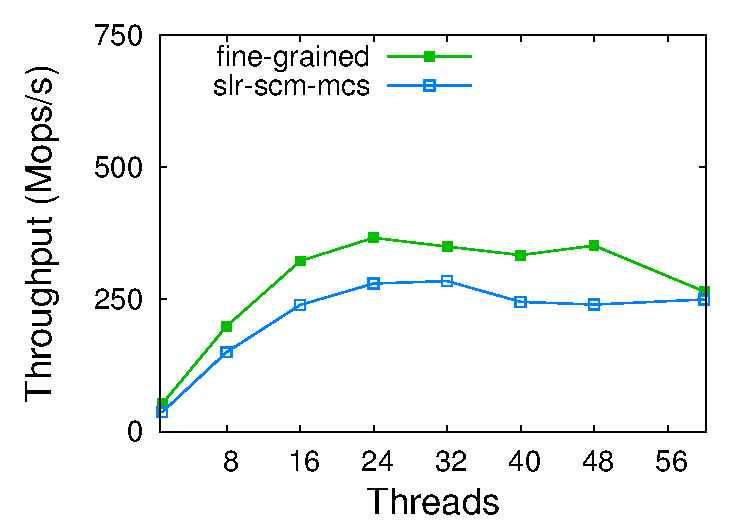
\includegraphics[width=0.45\textwidth]{Scal-u10-i1000(noset)}}
\subfigure[\textit{i} = 10$^6$]{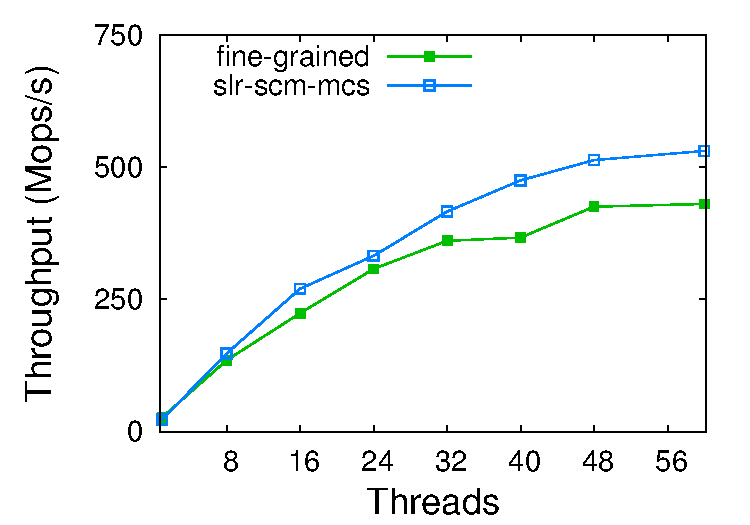
\includegraphics[width=0.45\textwidth]{Scal-u10-i1000000(noset)}}
\caption{传统细粒度锁方法和基于RTM的粗粒度锁方法之间的性能比较}
\label{fig:htm_coarse_grained}
\end{figure}

\textbf{分析}: 根据实验结果,总结了两点认识。
第一,在处理大规模工作集时,使用HTM构建并发哈希表的好处体现在两个方面:一是获得的性能和扩展性具有一定的竞争力;二是它能降低内存开销并达到简化并行编程的目的。
第二,当工作集的大小小于片上缓存的容量时,此时由于更加激烈的数据冲突引发频繁的事务中止影响了基于HTM的全局锁性能。

\subsection{不同的全局锁方案之间的比较}
进一步的评估使用不同的锁实现方式作为全局锁之间的性能差异。
为此实现了6种锁方法,它们分别是:
(1)标准的MCS锁,没有使用任何优化的MCS锁方法;
(2)用SLR优化的基于HTM的MCS锁(slr-mcs);
(3)基于HTM的事务重试方法(HTM-retry);不使用SLR和SCM进行优化,仅参照Intel技术手册上推荐的方法对发生中止的事务进行重试,重试的次数设定为10。
(4)使用SCM优化的基于HTM的ttas锁;
(5)采用SLR和SCM两种软件辅助方法共同优化的MCS锁(slr-scm-mcs);
(6)基于乐观的SCM方案的ttas锁,线程在经过10次重试事务执行后仍无法成功提交时,线程会以事务性的方式获取锁,完成本次操作。

图~\ref{fig:htm_global}~展示了运行初始化大小为1000和1百万两个级别的工作集的性能曲线。
\begin{figure}[htbp]
\centering
%\subfigure[Intel]{
\subfigure[\textit{i} = 10$^3$]{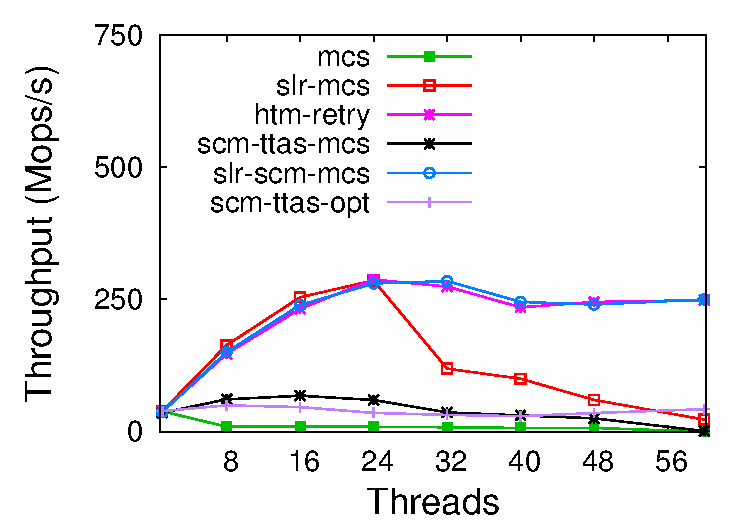
\includegraphics[width=0.45\textwidth]{coarse-grained-u10-i1000(noset)}}
\subfigure[\textit{i} = 10$^6$]{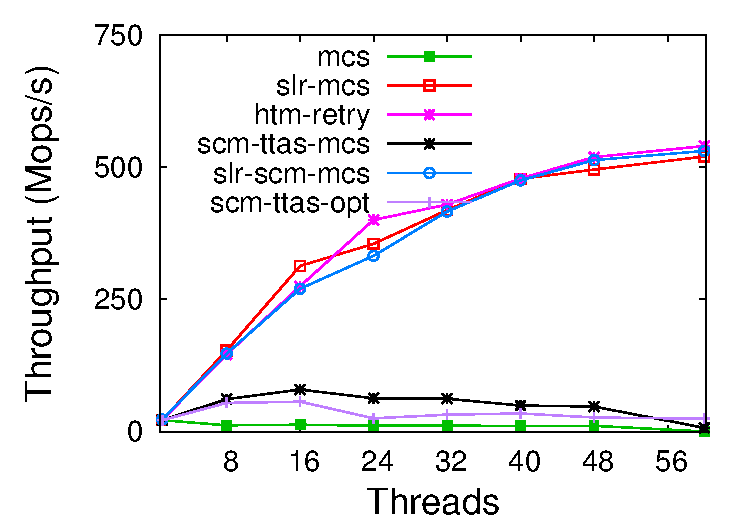
\includegraphics[width=0.45\textwidth]{coarse-grained-u10-i1000000(noset)}}
\caption{使用不同全局锁方法之间的性能比较}
\label{fig:htm_global}
\end{figure}
正如预期那样,使用传统的未经优化的MCS锁方法不论是线程扩展性还是性能都是集中方案种最差的。
从图~\ref{fig:htm_global}~(a)和(b)观察发现,当运行较小的工作集(初始化元素个数为1000)时,
slr-mcs,slr-scm-mcs和HTM-retries在\textit{n}为24时达到吞吐量峰值,之后吞吐量随着\textit{n}的增加而减少。
而其它两种方法,scm-ttas-mcs和scm-ttas-opt对应的性能只略微的比使用传统的MCS锁好一些。
在处理小规模数据时CLHT遭遇性能下降,原因是这种情况下触发数据竞争的概率是成倍增加的。
当数据集的大小超过最后一级缓存的容量时,slr-mcs, slr-scm-mcs以及HTM-retry三种方法都展现了近线性的线程扩展性。

在进行实验分析时还发现基于HTM实现的全局锁方法的CLHT的性能与线程绑定方式(三种线程绑定方式见~\ref{sec:thread_pinning}~)的影响。
这里采用紧凑型线程绑定方式。
图~\ref{fig:htm_pinning}~中描述了本次实验的结果。
\begin{figure}[htbp]
\centering
%\subfigure[Intel]{
\subfigure[\textit{i} = 10$^3$]{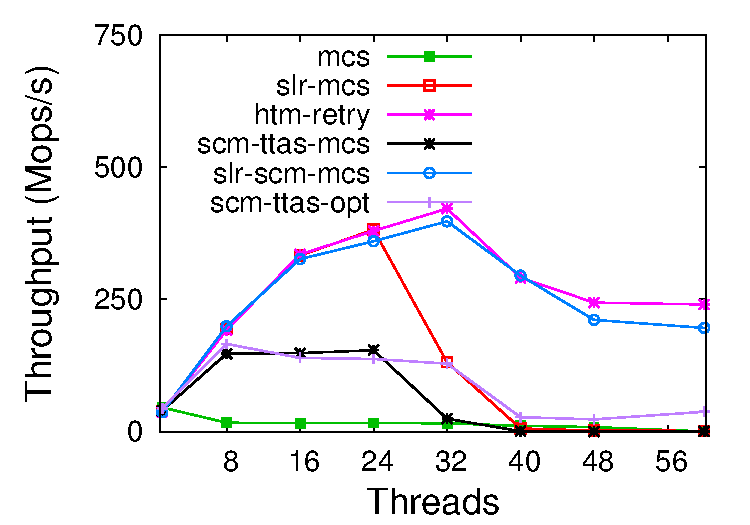
\includegraphics[width=0.45\textwidth]{coarse-grained-u10-i1000(setcpu)}}
\subfigure[\textit{i} = 10$^6$]{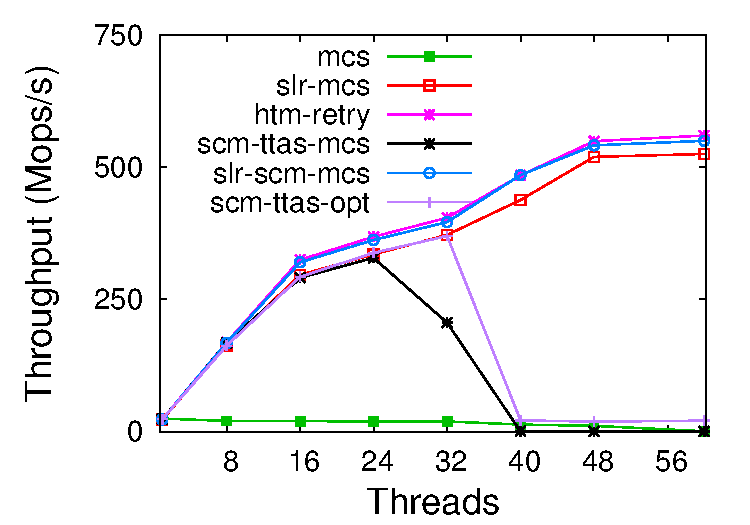
\includegraphics[width=0.45\textwidth]{coarse-grained-u10-i1000000(setcpu)}}
\caption{紧凑型线程绑定方案运行结果}
\label{fig:htm_pinning}
\end{figure}
通过与图~\ref{fig:htm_global}~的比较,有两个方面的发现:
其一,slr-scm-mcs, slr-mcs和HTM-retry三种方案的受线程绑定方式的影响较小,并且比其它几种方案的性能更加稳定。
其二,scm-ttas-mcs和scm-ttas-opt在单个socket内表现出较好的扩展性,然而当线程数量超过单个socket能够提供的最大线程数量时,它们的性能下降严重。
这种现象是由于它们在NUMA架构下,跨插槽通信的能力较弱引起的。

在~\ref{sec:htm_analysis}~中,将通过测算总的事务量、事务中止率以及发起锁请求的次数三个指标具体分析引起不同线程绑定方式之间性能差异的原因。

\textbf{分析}:从这一部分的实验中,得到的结论分为三个方面:
一是,MCS和HTM-retry同样是使用全局锁,后者是基于HTM的方法,未使用任何软件优化方案,两者之间的性能差异巨大,验证了硬件事务内存有助于激发多核处理器性能的说法;
二是,使用基于HTM实现的锁方法,能够在性能上有多大的提升取决于所使用的软件辅助优化技术;
第三,slr-scm-mcs和HTM-retry两种方案在扩展性上较其它方法更具有竞争力。


\subsection{基于HTM的细粒度锁实现与传统细粒度方法的比较}
使用基于HTM的全局锁构建并发哈希表有利于性能的提升。
还有一个令人关心的问题,如果使用基于HTM实现的锁用于构建并发哈希表会对性能提升有帮助吗?
下面将通过实验来回答这个问题。

参照实现基于HTM的粗粒度CLHT的实现方法实现了基于HTM的细粒度锁方法,并将其与原作者实现的细粒度版本在相同的测试平台上处理同样的工作集。
运行结果如图~\ref{fig:htm_fine_grained}~所示。
\begin{figure}[htbp]
\centering
%\subfigure[Intel]{
\subfigure[\textit{i} = 10$^3$]{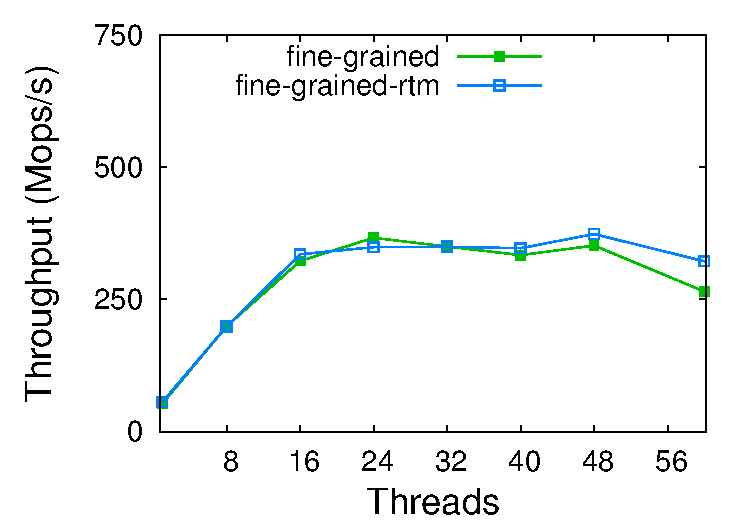
\includegraphics[width=0.45\textwidth]{fine-grained-u10-i1000}}
\subfigure[\textit{i} = 10$^6$]{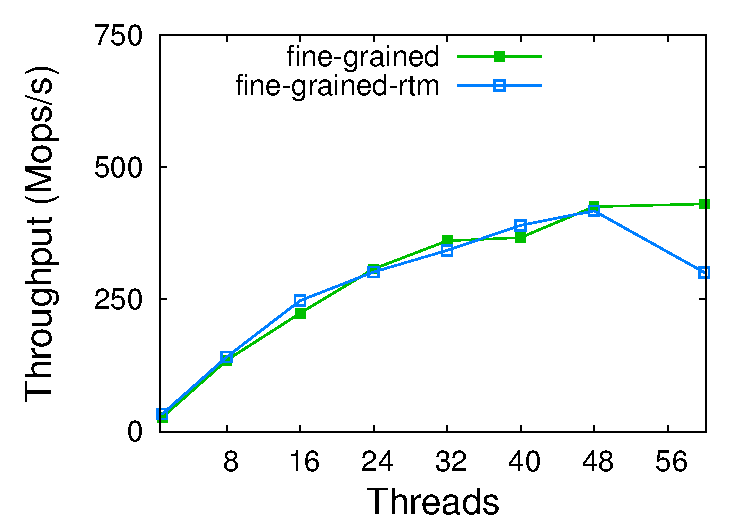
\includegraphics[width=0.45\textwidth]{fine-grained-u10-i1000000}}
\caption{使用/不使用HTM的细粒度锁方法之间的性能比较}
\label{fig:htm_fine_grained}
\end{figure}
通过比较得知,\textit{n} < 48时,两个版本间的性能差异并不明显。
产生这种现象的原因在于使用传统的细粒度的锁方法能够有效的避免在同一时刻多个线程同时访问相同内存地址。
因此,在这种情形下使用HTM对其进行优化以期获得更高性能的做法意义不大。
图~\ref{fig:htm_fine_grained}~(a)中,\textit{n} > 48时,使用HTM的CLHT的性能要略好于纯粹的细粒度锁方法。
原因是随着参与运算的线程数量的增加导致线程间的竞争更加激励,而HTM在数据冲突不是特别激烈的情况下是有利于提升并行化的。

\textbf{分析}:经过试验比较,得到的结论是:
在传统的细粒度锁方法能够提供良好的线程扩展性和性能的前提之下,使用HTM进行优化既达不到简化并发控制的目的,又对整体性能的提升没有助益。

\subsection{影响HTM性能的因素分析}
\label{sec:htm_analysis}

图~\ref{fig:htm_global}~展现了CLHT使用五个不同的基于HTM的同步方案的性能曲线,为了探究造成它们性能上的差异的原因,借助Intel的性能计数监视器(PMU)收集了一些微观的运行时指标。
这部分内容只挑选最能说明观察到的实验现象的指标予以说明。
表~\ref{tab:htm_abort_rate}~表中数据样本来自线程数为32,执行初始化大小分别为1百万/1000,更新比重为10\%的工作集。
表中第二列(c$_2$)数据表示运行中请求锁的次数,第三列(c$_3$)为发起的总的事务量,第4列(c$_4$)表示被中止的事务的数量,最后一列为中止率,通过c$_4$/c$_3$计算得到。
事务中止率\textit{r}由中止的事务量除以执行期间发起的总的事务量计算得到,总的事务量为中止的事务量与提交的事务量之和。
从表~\ref{tab:htm_abort_rate}~的数据中,观察发现不同的HTM方案对应的中止的事务量差别不大,表明中止的事务量并不是最主要的性能瓶颈,而执行中申请锁的次数以及发起的总的事务量直接对整体的性能造成影响。
申请锁的次数和提交的事务量越多,对应的吞吐量越高。
比如,slr-mcs,scm-ttas-mcs和HTM-retry对应的申请锁的次数和提交的事务量明显高于其它两种方案,正好对应图~\ref{fig:htm_global}~,这三种方法的性能曲线比另外两种更加理想。

\begin{table}[htbp]
  \centering
  \caption{Intel PMU收集的不同的HTM方法的运行时数据}
  \label{tab:htm_abort_rate}
  \begin{tabular}{ccccc}
    \toprule
                  & 申请锁的次数(百万) & 总的事务量(百万) & 中止的事务量 & 中止率(\%) \\
    \midrule
      HTM-retry   & 170/160           & 290/360         & 53/67      & 18.3/18.5 \\
      slr-mcs     & 160/60            & 290/360         & 52/67      & 18.6/18.6 \\
      slr-scm-mcs & 160/160           & 300/350         & 52/66      & 17.8/19.0 \\
      scm-ttas-mcs& 48/12             & 110/130         & 51/62      & 48.6/48.4 \\
      scm-ttas-opt& 110/48            & 220/180         & 53/65      & 23.0/35.4 \\
    \bottomrule
  \end{tabular}
\end{table}

此外,通过观察发现吞吐量随着中止率的升高而下降。
通过运行不同的参数组合来探究中止率、创建的线程的数量、更新比重以及哈希表初始化元素个数几者之间的关系。
表~\ref{tab:abort_rate_thread}~用以说明线程数与中止率之间的关系。
表~\ref{tab:abort_rate_thread}~的第二列和第三列分别表示发起的事务总量和被中止的事务量。
不论是发起的事务总量还是被中止的事务量都随着线程数量的增加而增加,然而被中止的事务量的增长速率远低于发起的事务量的增长速率。
换言之,随着越来越多的线程被创建用来参与运算,被提交的事务量的增长远远大于被中止的事务量的增长。
这个趋势与图~\ref{fig:htm_fine_grained}~中的线程的线程扩展性曲线相符合。

\begin{table}[htbp]
  \centering
  \caption{slr-scm-mcs方案的中止率随线程变化情况}
  \label{tab:abort_rate_thread}
  \begin{tabular}{cccc}
    \toprule
      \textit{n}  & 总的事务量(百万) & 中止的事务量 & 中止率(\%) \\
    \midrule
      2   & 156/156 & 70/66 & 43.6/42.3  \\
      8   & 228/239 & 72/59 & 31.6/21.5 \\
      16  & 303/298 & 73/64 & 24.1/19.5  \\
      32  & 382/349 & 80/67 & 20.9/19.2  \\
      40  & 399/299 & 77/74 & 19.3/24.8 \\
      48  & 495/310 & 87/78 & 17.6/25.2  \\
      64  & 522/316 & 90/89 & 17.2/26.0 \\
    \bottomrule
  \end{tabular}
\end{table}

表~\ref{tab:htm_update}~中的数据用以说明中止率随工作集中更新比重的变化情况。
线程数为32,表的第2到第4列表示的内容与表~\ref{tab:htm_abort_rate}~相同,每一列表中记录了两组数据,分别代表初始化值为1百万和1000时的测试结果。
这一次,运行的测试集中更新比重分别为0,10和80。
实验获得的结果是,运行不包含更新操作的工作集,对应的中止率也最低。
这是因为在纯读的场景下,没有写入内存的请求,这样发生数据冲突的概率很小,从而引起的事务中止也相对较少。
随着更新比重的增加,中止率会上升,随之而来的是性能的下降。

\begin{table}[htbp]
  \centering
  \caption{slr-scm-mcs方案的中止率随更新比重变化情况}
  \label{tab:htm_update}
  \begin{tabular}{cccc}
    \toprule
      \textit{n}  & 总的事务量(百万) & 中止的事务量 & 中止率(\%) \\
    \midrule
      0   &  346/554 & 73/60 & 21.1/10.8  \\
      10  &  320/352 & 70/66 & 21.9/18.8 \\
      80  &  282/273 & 74/70 & 26.4/25.6  \\
    \bottomrule
  \end{tabular}
\end{table}

\section{本章小结}
本章首先对事务内存、Intel TSX提供的两种接口——HLE和RTM——进行了介绍。提出了针对Intel TSX的两种软件优化方法:SLR和SCM。

然后,从对哈希表串行执行五次操作的实例入手,由浅入深的探讨了当前主流的三种同步锁模型:粗粒度锁,细粒度锁和硬件事务内存,在构建并发哈希表上的优势和劣势。
粗粒度锁方法实现简单,易于理解,且容易保障正确性,但是使用这种方法获得的性能很不理想。
细粒度锁方法能够发挥出多核系统的性能优势,并且有很好的线程扩展性,但是细粒度锁增加了设计并发哈希表的难度,并且需要花费大量精力在保证正确性上。
事务内存继承前两者的优势于一身,实现简单,易于验证正确性,又能够获得接近甚至超越细粒度锁方案的性能,是理想的并发编程范式。

接着,以基于细粒度锁的缓存行哈希为蓝本,使用SLR和SCM实现了基于硬件事务内存的并发哈希表,并就二者的性能进行了比较,证明了基于HTM的并发哈希表能够保证良好的线程扩展性和性能,并且在工作集较大的场景下,性能比细粒度锁实现更优。

实现了6种不同的粗粒度并发哈希,用于进一步的探究使用哪一种方法对基于HTM的并发哈希表的优化粒度更大。
并通过实验表明,在细粒度锁方案已经能够保证良好的性能和线程扩展性的前提下,使用HTM优化细粒度锁方案对于性能的提升没有意义。

最后,影响硬件事务内存性能发挥的因素进行了分析。通过测算测试过程中发起的事务总量、被中止的事务量以及中止率对实验评估中的一些现象进行解释说明。

对基于硬件事务内存的并发哈希表的评估结果表明,本章提出的方法达到了预期目标。
对于并发哈希表的设计具有重要的意义。

\chapter{支持动态更新的并发Cuckoo过滤器设计}
%引子
% 对于海量数据处理业务,通常需要建立索引数据结构来帮助查询,快速判断数据记录是否存在,过滤器(filter)能够很好的满足构建索引数据结构的要求。
查找或判断一个元素是否存在于一个指定集合中,这是计算机科学中一个基本问题。
通常会采用线性表(数组或链表)、树(二叉树、堆、红黑树、 B+/B-/B*树)等数据结构存储所有元素,对数据进行排序和查找。
这里的查找时间复杂性通常都是O(N)或O(log(N))。
如果集合元素非常庞大,不仅降低了查找的效率,同时对内存空间的需求也非常大。

在网络安全领域有一个简单的应用场景:判断URL是否链接到存在安全隐患的网站。
用户在浏览器内输入URL,浏览器需要判断该URL是否是恶意的,它将该URL与本地缓存的URL进行匹配,如果匹配失败,则说明该URL是安全的链接可以正常访问;否则,说明该URL可能存在安全隐患。
此时,提交请求给远程客户端进行验证,并警告用户该URL存在风险。
在这个应用场景中,如果缓存的URL数量很少,那么使用上述的数据结构都可以达到较高的查找效率,同时对内存空间的要求也不高。
假设现在需要缓存的URL的数量为10亿条(这在当前是很常见的一个数量级),每条URL的大小为8个字节,那么存储所有的URL大约需要8 GB的内存。
使用哈希表是一种可能的解决方案.哈希表的查询时间复杂度为O(1),可以节省查找的时间,但是没有降低对内存的需求。

事实上,除非有特别的需求,否者判断元素是否在一个指定集合内,并不需要把所有元素的原始信息都保存下来,而只需要保存该元素的“存在状态”,存储存在状态只需要几个bit。
使用哈希函数可以将元素映射成位数组中的一个点,采用k个哈希函数将元素映射成k个点。
这样,经过映射之后,查找元素是否存在时只需看看特定的几个位点的值就能判断某个元素是否存在于集合当中,如果k个位置都为1,则说明该元素可能存在,如果有1个位置上为0,则可以肯定该元素不存在。
这样不仅可大大缩减内存空间,查找速度非常
这就是布隆过滤器(Bloom Filter)的基本思想。
它的名字源自其发明者Burton.H Bloom\cite{bloom1970space}。
布隆过滤器最初应用于拼写检查和数据库系统。
但是,随着互联网的爆炸式发展,海量数据中快速检索目标数据的需求使得布隆过滤器的应用焕发新生,涌现出新的应用和变种\cite{bender2012don,bonomi2006improved,song2005fast,yu2009buffalo}。

\section{布隆过滤器}

\subsection{基本原理}
布隆过滤器使用位数组表示元素集合S,并使用k个哈希函数(h$_1$, h$_2$, ..., h$_k$)来对元素进行位映射。
初始状态下的布隆过滤器是一个包含m位的位数组,每一位都置0,图~\ref{fig:bf}(a)所示为m = 12的布隆过滤器。
当需要将集合S中的n个元素x$_1$,x$_2$, ... x$_n$用位数组表示时,对该元素分别使用k个相互独立哈希函数进行计算,得到位数组上k个位置的索引值,随后将映射到位数组的相应位置1。
值得注意的是,如果一个位置被多次置为1,只有第一次的置位是有效的。
图~\ref{fig:bf}(b)表示k = 3时,将元素映射到位数组的过程,其中元素x$_1$和x$_2$都对第5位置位。
图~\ref{fig:bf}(c)表示判断元素y$_i$(i = 1,2, ..., n)是否属于集合。
与插入过程类似,同样先对y进行k次哈希,如果计算得到的索引值对应的位上有任何一位为0则表示y元素绝对不存在于集合中,只有当所有映射位均为1时才表示该元素\textbf{有可能}存在于集合当中。
\begin{figure}[htbp]
\centering
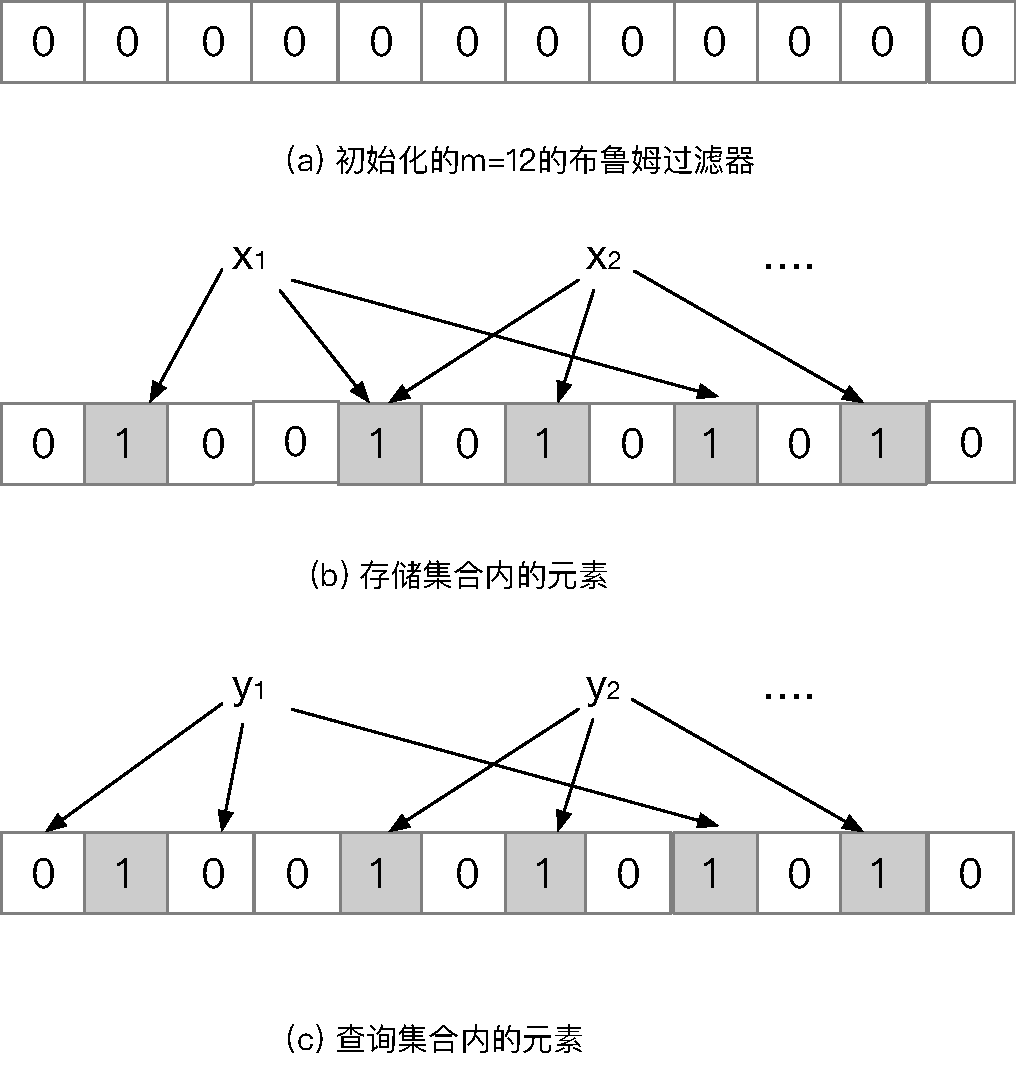
\includegraphics[width=0.65\textwidth]{bloomfilter}
\caption{布隆过滤器}\label{fig:bf}
\end{figure}
换句话说,如果布隆过滤器判断一个元素不在集合中,那肯定就不存在;而如果判断存在,则不一定存在,下文将对这种不一定存在的原因进行说明。
这种不能确定元素一定存在的问题是由哈希函数可能发生碰撞的特性所决定的。
这个错误率可调整位数组大小或者哈希函数个数进行控制。
由此可见,布隆过滤器的高效是以一定的误报为代价的,它通过容忍一定的错误发生的概率换取存储空间的极大节省。
布隆过滤器不适合那些“零错误”的应用场合。

标准的布隆过滤器不支持删除操作。
原因很简单,考虑在图~\ref{fig:bf}(b)中删除元素x$_2$,意味着将位数组内的第5、7、11位置0,此时如果查询x$_1$会发现也不存在,因为它对应的第5位上的值在删除x$_2$时被置0了。

标准布隆过滤器的实现中有几个重要参数:误判率\begin{math}\epsilon\end{math}、负载因子\begin{math}\alpha\end{math}、哈希函数的个数k、位数组大小m和集合中元素的个数n。下面将对这些参数进行推导,以确定实现标准布隆过滤器的参数选取原则。

\subsection{误判率估计}
在进行正式的误判率估计前先明确几个定义和重要的参数:
\begin{definition}
	假阳性(false positives)也叫误判是指当前元素不在集合内,但由于哈希冲突的缘故存在其它元素被映射到部分相同bit位上,从而有一定的概率导致在判定该元素时认定其对应的所有位置都为1,从而判定其在集合内,造成一次误判。这个概率本文称为误判率,误判率用\begin{math}\epsilon\end{math}表示。
\end{definition}

\begin{definition}
	假阴性(false negatives),也叫漏报,是指在位数组内删除某个元素,导致该元素对应的比特位置0,造成本来存在的元素会被漏报成不存在。
\end{definition}

\begin{definition}
	负载因子是指集合中的元素的个数\textit{n},布隆过滤器位数组的位数\textit{m}之间的比值,它用\begin{math} \alpha \end{math}表示,其中\begin{math} \alpha  = {n/m} \end{math}。当\begin{math} \alpha \end{math}为0时,表示布隆过滤器为空,\begin{math} \alpha \end{math}为1表示布隆过滤器满载。
\end{definition}

下面进行误判率\begin{math}\epsilon\end{math}的推算.
首先假设布隆过滤器中使用的k个哈希函数的计算结果都是均匀分布的,即每个元素都等概率地被哈希到m个bit位上的任何一个,与其他元素被哈希到的位置无关。
则对某一特定bit位在一个元素由特定哈希函数插入时没有被置位为1的概率p$_1$为:
\begin{equation}
p_1 = 1-{1/m}
\end{equation}
则k个哈希函数中都没有一个对其置位的概率p$_2$:
\begin{equation}
p_2 = {p_1}^k
\end{equation}
如果插入n(\begin{math}n\leqslant m\end{math})个元素,但都未对其置位的概率p$_3$:
\begin{equation}
p_3 = {p_2}^n = {p_1}^{kn}
\end{equation}
则此位被置位的概率p$_4$为:
\begin{equation}
p_4 = 1 - \left(1 - {1/m}\right)^{kn}
\label{equ:alpha}
\end{equation}
现在考虑判定阶段,若对应某个判定元素的k个位全部置位为1,则可判定其在集合中。因此将某元素误判的概率为:
\begin{equation}
\epsilon = \left(1 - \left(1 - {1/m}\right)^{kn}\right)^k
\label{equ:epsilon}
\end{equation}


由
\begin{math} \left(1 + x\right)^{{1/x}} \thickapprox e \end{math}
可知,但m很大时,满足
$-{1/m}$ $\to 0$,
可将公式\ref{equ:alpha}转化为:
\begin{equation}
\epsilon = \left(1 - \left(1 - {1/m}\right)^{{-m}\frac{-kn}{m}}\right)^k \thickapprox \left(1 - e^{-\frac{nk}{m}}\right)^k
\label{equ:beta}
\end{equation}
由公式\ref{equ:beta}可以初步断定\begin{math}\epsilon\end{math}与元素的个数n和位数组的长度m决定,增大n或者减小m都会导致\begin{math}\epsilon\end{math}的升高。这种计算方法不严格,因为前面假设哈希函数和散列后值的分布是相互独立的。
但是,这个假设随着m和n的增大误判率更接近真实的误判率。
Mitzenmacher证明无假设情况下的误判率的期望值相同\cite{mitzenmacher2002compressed}。

\subsection{最优哈希函数个数}
\label{sec:num_hashf}
哈希函数的选择对于布隆过滤器的性能以及空间利用率都有至关重要的作用。
对于选取什么样的哈希函数已经在前文中有过介绍,这里不再缀述。
而对于哈希函数的个数,直观的认为越多越好。实际上,哈希函数越多,用于表达集合中每一个元素所需要的位数就越多,这与布隆过滤器用较低的误判率换取空间的高效利用的初衷相悖。那么哈希函数的个数应该满足什么条件才能有最佳性能呢?

下面推导对给定的$\alpha$,k满足什么条件可以使$\epsilon$最小化。

令:
\begin{equation}
f\left(k\right) = \left(1 - e^{-{nk/m}}\right)^k 
\end{equation}

取 b = e$^{n/m}$,得:
\begin{equation}
f\left(k\right) = \left(1 - b^{-k}\right)^k 
\end{equation}

两边取对数得: 
\begin{equation}
lnf\left(k\right) = kln\left(1 - b^{-k}\right)
\end{equation}

函数两边对k求导得:
\begin{equation}
{1/f(k)}\cdot f'(k) = ln(1 - b^{-k}) + k \frac{b^{-k}\cdot lnb}{1 - b^{-k}} 
\label{equ:fk}
\end{equation}

对式~\ref{equ:fk}右边求最值。

令:
\begin{equation}
\begin{split}
\frac{1}{f(k)}\cdot f'(k) = ln(1 - b^{-k}) + k\cdot \frac{b^{-k}\cdot lnb}{1 - b^{-k}} = 0 \\
\Rightarrow (1 - b^{-k}) ln(1 - b^{-k}) = -k\cdot b^{-k}\cdot lnb \\
\Rightarrow 1 - b^{-k} = b^{-k} \\
\Rightarrow e^{-\frac{kn}{m}} = \frac{1}{2}\\
\Rightarrow k = ln2\cdot {m/n} \thickapprox 0.7{m/n}
\end{split}
\end{equation}
因此,对于固定的$\alpha$,当$k = 0.7{m/n}$时具有最低的误判率,此时$\epsilon$等于:
\begin{equation}
(1 - {1/2})^k = 2^{-ln2\cdot\frac{m}{n}} \thickapprox 0.62{m/n}
\end{equation}

\subsection{最优位数组长度}
\label{sec:opt_m}
下面进行给定一定的误判率上限,布隆过滤器至少需要多少位才能表示全集中任意的x个元素的集合。
假设全集中元素的个数为n,最大误判率为$epsilon$。以此为前提展开对位数组大小的推导。

假设$S_n$为全集中任取$n$个元素的集合,$B$是表示$S_n$的位数组。
那么对于集合$S_n$中任意一个元素$x$,在$B$中查询$x$都能得到肯定的结果,即$B$能够接受$x$。
显然,由于布隆过滤器引入允许误判,$B$能够接受的不仅仅是$S_n$中的元素,它还允许最多$\epsilon \cdot(u - n)$个误报。因此,对于一个确定的位数组来说,它能够接受总共$n +\epsilon\cdot(u - n)$个元素。在$n + \epsilon\cdot(u - n)$个元素中,$B$真正表示的只有其中$n$个,所以一个确定的位数组可以表示:
\begin{equation}
\binom{n + \epsilon \cdot(u - n)}{n}
\end{equation}
个集合。$m$位的位数组一共有$2^m$个不同的组合,可以进一步推导$m$位的位数组可以表示:
\begin{equation}
2^m\binom{n + \epsilon *\left(u - n\right)}{n}
\end{equation}
个集合。全集中包含n个元素的子集总共有:
\begin{equation}
\binom{u}{n}
\end{equation}
个。因此,要让布隆过滤器的位数组大小能够满足所有包含n个元素的子集,必须满足:
\begin{equation}
2^m\cdot\binom{n + \epsilon \cdot(u - n)}{n} \geq \binom{u}{n}
\end{equation}
即m需要满足:
\begin{equation}
m \geq log_2({\binom{u}{n}/\binom{n + \epsilon \cdot(u - n)}{n}}) \geq log_2({\binom{u}{n}/\binom{\epsilon u}{n}}) \thickapprox log_2\epsilon^{-n} = n log_2({1/\epsilon})
\label{equ:bfm}
\end{equation}
式~\ref{equ:bfm}中近似相等有个重要的前提条件:$n$远小于$\epsilon\cdot u$,这个前提在实际的问题中也是常见的。
根据式~\ref{equ:bfm}中的不等式,得到如下结论:在误判率上限为$\epsilon$的情况下,$m$至少要等于$nlog_2{1/\epsilon}$才能表示任意$n$个元素的集合。

在本章~\ref{sec:num_hashf}中推导出哈希函数的个数$k$等于$k = 0.7{m/n}$时可以得到最小误判率,此时的误判率为$(\frac{1}{2})^{0.7{m/n}}$。
令$(\frac{1}{2})^{0.7{m/n}} \leq \epsilon $,可以进一步推导:
\begin{equation}
m \geq n\frac{log_2({1/\epsilon})}{ln2} = nlog_2e\ast log_2({1/\epsilon}) \thickapprox 1.44n\cdot log_2({1/\epsilon})
\label{equ:bfm2}
\end{equation}

式~\ref{equ:bfm2}说明当k取到最优值时,要保证误判率不超过给定的上限$\epsilon$,$m$至少要取到最小值的1.44倍。
可以验证,当给定$\epsilon = 0.01$时,存储每个元素需要9.6比特。
而将$\epsilon = 0.001 $时,每个元素需要额外的增加4.8比特。
所以,在实际的应用中,对于误判的容忍度不同,要求误判率越低,则存储每个元素需要的比特位越多,相同容量下存储的元素个数就越少。

\section{Cuckoo过滤器的参数}
\label{sec:cbf_para}
传统的布隆过滤器的空间效率高,对插入和查询元素的处理也相当快。
但是它也存在缺陷——存在一定的误报率,不支持元素的删除操作。
消除误报率除非能实现没有碰撞的哈希函数,但是不发生碰撞的哈希函数至今没有被设计出来。
研究人员能做的就是尽量选择均匀的哈希函数,并且借助一些数据结构的特性有效的对碰撞进行处理。
而在上一节的中介绍到误判率每缩小到原来的十分之一,至少要增加4.8个比特位用于表示一个元素。
另外,实现元素删除操作的一个方法是引入计数器,将每个比特位都扩张成一个计数值,降低了空间效率。
为了支持对元素的删除操作,出现了很多标准布隆过滤器的扩展版本\cite{bender2012don,bonomi2006improved,fan2000summary}。
所以,布隆过滤器实现更低的误判率和实现删除操作都需要牺牲一定的空间效率。

为了解决上述问题,本文引入一种新的数据结构——Cuckoo过滤器。
它既可以确保该元素存在的必然性,即将“可能存在”变成“一定存在”;
又支持动态的对元素的插入和删除,而不会造成漏报。

为了支持动态的插入和删除元素,Cuckoo过滤器采用的是一种称为\textbf{不完整键值(partial-key)} Cuckoo哈希的技术。
Cuckoo过滤器是标准Cuckoo哈希表在集合元素查询算法领域的应用。
在前面的章节中已经对Cuckoo哈希表的基本原理和概念有过详细介绍(\textcolor{red}{第~\ref{sec:XX}节}),这里不再赘述。
仅对与在这一部分密切相关的术语进行重申。
Cuckoo的数据结构与Cuckoo哈希表相同,其基本单元称为\textbf{实体}(entry),不同的是每一个实体内存储的不是完整的键值,而是根据键值进行提取后的\textbf{指纹}(fingerprint)~\cite{memc3},用$f$表示。
哈希表由存储了多个实体的\textbf{桶}(bucket)数组构成。

表~\ref{tab:ckf_para}列出了本小节所用到的一些关键参数及其含义。
\begin{table}[htbp]
  \centering
  \caption{相关符号及其含义}
  \label{tab:ckf_para}
  \begin{tabular}{cc}
    \toprule
      参数  & 含义  \\
    \midrule
      $\epsilon$  					  &   误判率 \\
        f 							  &   指纹信息的长度(单位:bit)\\
      $\alpha$					      &   负载因子($0\leq\alpha\leq 1$) \\
    	b                             &   每个哈希桶内包含的实体的数量 \\
    	m 							  &	  哈希桶的数量 \\
    	n                             &   元素的数量 \\
        C 							  &   表达一个元素所需的平均位数(单位:bit)\\
    \bottomrule
  \end{tabular}
\end{table}

\subsection{指纹信息的长度}
在这一部分中,将探讨构造Cuckoo过滤器的几个关键参数。
在Cuckoo过滤器中使用不完整键Cuckoo哈希方法存储指纹信息会导致指纹信息的下界值随着过滤器大小的增加而缓慢增加。
这与用传统方法实现的过滤器相反,在标准布隆过滤器中,指纹信息的大小只与预定的$\epsilon$有关。这个看上去似乎是Cuckoo过滤器的劣势,实际上它造成的影响微乎其微。

\subsubsection{指纹信息下界约束}
在Cuckoo过滤器中,对于一个给定的元素,根据其当前位置和指纹信息使用不完整键哈希方法可以推导出它的备选哈希桶的索引值。
这样,每个元素的候选哈希桶都不是独立的。
比如,某一元素可以存放在桶$i_1$或$i_2$中,对于长度为$f$比特的指纹信息,根据公式~\ref{equ:ckf},$i_2$可能的索引值最多有$2^f$种可能。
若指纹信息的长度为一个字节,对给定的$i_1$,$i_2$最多只能偏离$i_1$ 256个位置。
对于具有$m$个桶的哈希表而言,当$2^f \leq m$时,$i_2$能够选择的哈希桶的范围只是整个$m$个哈希桶的一个很小的子集。
这会引起更多的碰撞。

直观上看如果指纹信息的长度足够长,不完整Cuckoo哈希仍然能够接近标准Cuckoo哈希的冲突处理能力。
然而,如果哈希表非常大,而此时指纹信息的长度相对来说要远远小于哈希表的大小,这样容易引起更多的哈希碰撞,从而导致插入失败的概率升高。
当Cuckoo过滤器需要处理大量元素,而$\epsilon$设定一个s中等偏低的值时,可能发生上述情形。
接下来,将通过分析确定插入失败的概率下限。

首先推导对于给定的$u$个元素,它们恰好映射到相同的两个哈希桶内的概率$p_1$。
假设第一个元素$x$位于桶$i_1$内,并且指纹为$t_x$。
如果其他的$u-1$个元素具有与$x$相同的桶索引值,它们必然满足以下两个条件:(1)它们的指纹都为$t_x$,出现的概率为$\frac{1}{2^f}$;
(2)它们第一个桶索引值为$i_1$或者$i_1 \bigoplus h(t_x)$,出现的概率为$\frac{2}{m}$。
因此,$u$个元素映射到相同的两个桶内的概率$p_1 = (\frac{2}{m}\ast \frac{1}{2^f})^{u-1}$

现在考虑构建Cuckoo过滤器的随机插入$n$个元素的构建过程。
假设初始化的哈希表桶数组满足$m = cn$,每个哈希桶容纳的元素个数为$b$,其中$c$为常数。
当出现$u = 2b+1$个元素被映射到相同的两个桶内时,插入失败。
这个概率为插入失败的概率下界。
由于从$n$个元素中包含$2b+1$个元素的子集有$\binom{n}{2b+1}$个,$2b+1$个元素在插入过程中发生碰撞的期望值为:
\begin{equation}
\binom{n}{2b+1}(\frac{2}{2^fm})^{2b} = \binom{n}{2b+1}(\frac{2}{2^f{cn}})^{2b} = \Omega(\frac{n}{4^{bf}}) 
\label{equ:cbf_f}
\end{equation}

因此,由式~\ref{equ:ckf_f}可以做出结论,$4^{bf}$必须满足$\Omega(n)$才能避免一场的插入失败的概率。
指纹信息的长度最好为$f = \Omega(log(\frac{n}{b}))$比特。
在第~\ref{sec:opt_m}节中指出标准的布隆过滤器用于表示每个元素所需的比特数为常数(近似等于$ln(\frac{1}{\epsilon})$)。
而Cuckoo过滤器指纹信息所需的长度为$\Omega(logn)$这个级别,这个结果看上去似乎不是特别理想。
这会不会引起扩展性问题呢?
实验表明桶容量$b$的在下界约束中的起决定作用:只要将$b$控制在合理的大小,指纹信息的长度仍然可以保持较小的值。

\subsubsection{实验评估}
%实验评估
图~\ref{fig:cbf_fingerprint_size}所示为负载因子与指纹信息长度$f$,哈希桶容量$b$以及哈希表总的哈希桶数量$m$的数量关系曲线。
$x$轴表示指纹信息的大小($1~\leq ~f~\leq ~20$),$y$轴表示负载因子($0~\leq ~\alpha ~\leq 1$)。
图~\ref{fig:cbf_fingerprint_size}(a)、(b)所示分别为$b = 4,8$时指纹信息长度与负载因子的变化关系。
实验时,插入的键为64位的随机值。
认定哈希表“饱和”的条件是:当执行某次插入操作时,进行了多达500次的替换操作之后仍没有找到空闲的位置接纳被踢出的元素。
当哈希表达到”饱和“之后,停止本次测试并记录此时哈希表的负载因子。
每组参数运行十次,最终结果取十次的平均值。
\begin{figure}[htbp]
\centering
\subfigure[$b$~= ~4 ]{\includegraphics[width=0.45\textwidth]{cbf_loadfactor_b4}}
\subfigure[$b$~ = ~8]{\includegraphics[width=0.45\textwidth]{cbf_loadfactor_b8}}
\caption{负载因子与指纹信息长度变化关系}
\label{fig:cbf_fingerprint_size}
\end{figure}

如图~\ref{fig:cbf_fingerprint_size}所示,在所有的参数组合中,$b = 4$的过滤器的哈希表的利用率能够达到95\%,而$b = 8$的过滤器在指纹信息大小足够长的前提下哈希表利用率可以达到98\%。利用率达到这些值后,增加指纹信息的长度对哈希表利用率的提升几乎没有帮助(但是可以降低误判率)。
通过前文的理论分析表明,当过滤器的规模增大时,所需的$f$的最小值会发生变化。
此外,通过比较图~\ref{fig:cbf_fingerprint_size}(a)和图~\ref{fig:cbf_fingerprint_size}(b)发现达到高哈希表利用率的$f$的最小值随着哈希桶容量$b$的增加而减小,这个规律同样的也与前文的理论推算吻合。
在本次实验中,使用两个完全独立的哈希函数,当$b = 4$且$m = 2^{30}$时,哈希表最多能存储多达40亿个元素,而当指纹信息的长度大于6比特时,$\alpha$接近"最优负载因子"。

\subsubsection{启示}
通过结合公式~\ref{equ:cbf_f}对$f$的下界约束推导的结果与图~\ref{fig:cbf_fingerprint_size}中的实验结果可以总结出Cuckoo过滤器的一条非常重要的结论。
在理论上Cuckoo过滤器的空间效率要比标准布隆过滤器“差”——
$\Omega(log~n)$与常数间的区别。
对于布隆过滤器而言,不论哈希表存储的元素个数是一千、一百万还是数十亿,达到百分之一的误判率大约都只需要10个比特位来表示每个元素。
而为了保持相同的空间效率Cuckoo过滤器需要使用更多的比特位表示每条指纹信息。
同样的由理论推算过程可知,$f$为$\Omega(log~n)$比特,如果$b$足够大,则$f$的值增长非常缓慢,在实际的应用中,可以将其视为常数。
图~\ref{fig:cbf_fingerprint_size}的结果表明6比特的指纹信息足够存储数十亿个元素,并且能够达到很高的哈希表利用率。

\subsection{空间效率}
对Cuckoo过滤器内的元素进行增、删、查操作与每个哈希桶内包含多少实体无关。
但是,为Cuckoo过滤器选择正确的参数对于空间效率具有重要意义。
这一部分着重介绍如何选取合适的参数优化Cuckoo过滤器的空间效率。

\subsubsection{空间开销}
空间效率是通过计算在完整的过滤器中用于表示每个元素所用的平均比特数来衡量的。
用哈希表的大小除以过滤器有效存储的元素的个数就是表示每个元素所用的平均比特数。
尽管每个实体可以存储一条指纹信息,但是并不是所有的实体都已经存入了指纹信息——过滤器的哈希表内一定有空闲的实体。
所以,每个元素实际上需要的比特数大于指纹信息的长度。
如果每条指纹信息的长度为$f$比特,哈希表的负载因子为$\alpha$,则每个元素的空间开销C为:
\begin{equation}
C = \frac{\text{哈希表的大小}}{\text{元素个数}} = \frac{f\cdot \text{实体数量}}{\alpha \cdot \text{实体的数量}} = \frac{f}{\alpha} \text{bits.}
\label{equ:space_cost}
\end{equation}

在前文中有过介绍,指纹信息的长度和负载因子都与哈希桶的大小有关。
下面研究在给定的误判率$\epsilon$前提下,如何通过选取最优的桶大小$b$使$C$最小化。

保持Cuckoo过滤器的总的大小为常量,改变哈希桶的大小会产生两方面的影响:
\begin{itemize}
\item \textbf{哈希桶容纳的实体数量越多,哈希表的空间占用率就越高。}对于使用两个哈希函数的Cuckoo过滤器,当桶能容纳的实体数$b = 1$时,哈希表的负载因子$\alpha$为50\%,
而当$b = 2,4,8$时,$\alpha$分别为84\%,95\%和98\%。
\item \textbf{哈希桶的容量越大,维持相同$\epsilon$需要的指纹信息的长度越长。}
哈希桶的容量越大,进行查询时需要检查更多的实体,并且发现相同指纹信息的概率也会增加。
在最坏情况下,查询一个并不存在的元素需要探测两个分别包含了$b$个实体的桶
(当然并不是所有的哈希桶内都填满了实体,这里只是考虑最糟糕的情况;当哈希表的负载因子达到95\%时,已经很接近极限情况)。
对于每一个实体而言,一次查询与存储的指纹相匹配并且返回成功匹配误报的概率最多为${1/2^f}$。
在进行$2b$次这样的比较之后,误报率的上界为:
\begin{equation}
1 - (1 - {1/2^f})^{2b} \thickapprox {2b/2^f}
\end{equation}
该上界约束与哈希桶的容量$b$成正比。
为了保证预定的误报率$\epsilon$不变,必须确保${2b/2^f}\leq \epsilon$,保证这个条件的最小指纹信息长度为:
\begin{equation}
f \geq \lceil log_2({2b/\epsilon})\rceil = \lceil log_2({1/\epsilon}) + log_2(2b)\rceil  
\label{equ:upper_f}
\end{equation}
\end{itemize}

由式~\ref{equ:space_cost}和\ref{equ:upper_f}可以推算存储每个元素的空间开销$C$受下面条件的限制:
\begin{equation}
C \geq {\lceil log_2({1/\epsilon}) + log_2(2b)\rceil /\alpha}
\label{equ:space_cost_bound}
\end{equation}
$\alpha$随着$b$的增加而增加。
当$b = 4$时,$\alpha = 0.95$,${1/\alpha} \thickapprox 1.05$。
此时$C$ = 1.05$log_2({1/\epsilon}) + 1.05\cdot 3$。
式~\ref{equ:space_cost_bound}表明,当负载因子一定时,Cuckoo过滤器的空间开销要低于布隆过滤器($1.44log_2({1/\epsilon})$)。

\textcolor{red}{为了确定最优的哈希桶容量$b$,下面将通过实验比较参数$b$为不同的值时的空间效率。
用不完整键Cuckoo哈希方法构造具有不同的指纹信息长度的哈希表,分别记录对应的平均空间开销和误判率。
结果如图~\ref{fig:cbf_opt_b}所示。
使空间效率最好的$b$的取值依赖于预定的误判率$\epsilon$:当$\epsilon > 0.002 $时,$b = 2$对应的平均空间开销要略好于$b = 4$对应的空间开销;而当$ 10^{-5} < \epsilon \leq 0.002$时,$b = 4$具有最小的空间开销。}

综上所述,Cuckoo过滤器的默认参数配置为(2,4),即每个元素有两个候选的哈希桶,每个哈希桶最多能够容纳4条指纹信息。
选取这组参数作为默认配置的原因一是实际的应用一般都要求$ 10^{-5} < \epsilon \leq 0.002$~\cite{broder2004network},二是这个参数组合能够提供最优综合性能。

\section{并发Cuckoo过滤器}
无论是标准的布隆过滤器还是现有的其他一些布隆过滤器的扩展版本,都具有在单核平台上快速处理元素的能力以及高效的空间利用率。
单核处理器的计算能力已达到瓶颈,相对而言多核计算机的计算资源和计算能力更加充裕。
在当前数据呈现爆炸式增长的背景下,海量数据处理压力越来越大,单核处理器上的过滤器逐渐显得捉襟见肘。
因此,设计基于多核系统的多线程并发的过滤器对于海量数据处理无疑是雪中送炭。
然而,当前的相关研究中并没有一款支持多核并发查询和更新的过滤器。

并发控制在多核平台上设计并发数据结构的关键环节,它对线程扩展性和整体性能起决定作用。
在前面对并发哈希表的评估与分析中通过比较各个并发哈希表的线程同步方式发现不当使用共享变量以及使用TAS锁不利于并发哈希表的线程扩展性。
本文设计的并发Cuckoo过滤器其基础数据结构本质上仍然是哈希表,不同的是Cuckoo过滤器结合了处理集合成员查询问题的特征改用存储不完整键值替换标准Cuckoo哈希表中存储完整的键值信息的做法,换取存储空间的极大节省。
因此,前文通过实验评估得出的结论仍然适用于并发Cuckoo过滤器。

在这个背景下,设计了一种支持多核并发的基于不完整键Cuckoo哈希方法的过滤器。
这一部分主要介绍并发Cuckoo过滤器的实现过程和性能评估结果。

\subsection{加锁与解锁}
接下来的内容介绍如何通过基于Intel RTM的MCS锁实现多线程并发的Cuckoo过滤器。
Listing 2.1 给出了基于Intel RTM的MCS锁算法实现。
$locklib\_mutex\_t$是一个包含了MCS锁字段、一个$uint8\_t$类型的$mode$变量以及一个用于缓存行对齐的字符串的结构体。
函数$locklib\_mutex\_lock()$具有两个参数,一个为互斥量$mutex$,一个为整型数$mode$。
$mode$的值分别对应0、1,0表示当前持有锁的操作为读取操作,1表示当前持有锁的操作为更新操作(删除或插入)。
\begin{lstlisting}[caption = {基于Intel RTM的MCS锁算法}]
struct {
        mcs_lock_t    lock;
        uint32_t    pad1[128/4 - sizeof(mcs_lock_t)];
} spec_mcs_lock_t;

struct {
        mcs_lock_t        mcs;
        uint8_t mode;
        char padding[];
} locklib_mutex_t;

int locklib_mutex_lock(locklib_mutex_t *mutex, uint8_t mode){
        spec_mcs_lock_t *lock = (spec_mcs_lock_t *) mutex;
        uint32_t reason = 0;

speculative_path:
        XBEGIN(fallback_path, reason);
        if (lock->lock) XABORT(1);
        return 0;

fallback_path:
        retries++;
        while (lock->lock)
                cpu_relax();
        if (retries < MAX_RETRIES)
                goto speculative_path;

        // Acquire lock in a standard manner
        my_node.locked = true;
        qnode_t *prev = __sync_lock_TAS(&lock->lock, &my_node);
        if (unlikely(prev != NULL)) {
                prev->next = &my_node;
                while (my_node.locked)
                        cpu_relax();
        }
        mutex->mode = mode;
        return 0;}
\end{lstlisting}
对临界区的保护设置了$speculative\_path$,$fallback\_path$两条执行路径:一条为事务化推测执行路径(第16行);一条为回退路径(第21行),即当事务执行失败后,临界区申请标准锁完成本次操作。
在事务化推测执行期间,线程首先不会申请获取锁,直到执行完成准备提交时再申请获取锁,如果申请的锁被占用,则该线程所执行的事务被中止,
线程对系统状态所做的更改都失效,系统回退到初始状态跳转到回退路径执行(事务内存的原子性)。

跳转到回退路径之后,如果当前重试的次数没有达到预先设定的门限值,将继续尝试进行事务化推测执行(第23-26行)。
如果当前重试次数已经达到了门限值,则使用标准的锁方法完成操作(第29-35行)。

由于硬件事务内存不能保证每次事务化执行都能成功提交对系统状态的更改,为了避免进程悬停,在使用硬件事务内存进行锁省略编程时设置回退路径是有效的保障程序顺利执行的手段。
一般的,事务代码在经过一定次数的重试之后成功提交的概率远远大于失败的概率,所以执行回退路径对性能的影响是可控的。

% \begin{figure}
\begin{lstlisting}[caption = {基于Intel RTM的MCS解锁算法}]
int locklib_mutex_unlock(locklib_mutex_t *mutex)
{
    spec_mcs_lock_t *lock = (spec_mcs_lock_t *) mutex;

    if (XTEST()) {
        XEND();
    } 
    else {
        // Release lock in a standard manner
        qnode_t *last = my_node.next;
        if (last == NULL) {
            if (likely(true == __sync_bool_CAS
            	(&lock->lock, &my_node, NULL)))
                	return 0;

            while ((last = my_node.next) == NULL)
                	cpu_relax();
            }

        my_node.next = NULL;
        last->locked = false;
    }

    retries = 0;
    return 0;
}
\end{lstlisting}

Listing 2.2 展示了对应的解锁过程。
与加锁过程的两条路径相对应,释放锁的过程也分为两个阶段:首先使用\textit{XTEST}判断当前执行的操作是否为事务执行,若为事务执行,使用\textit{XEND}结束;若判断此次操作申请的锁是通过标准的方式获取的,则按照标准锁的释放过程释放锁。
最后将\textit{retries}变量清零。

\subsubsection{并发访问接口}

\begin{table}[htbp]
  \caption{HashTable类的成员函数列表}
\label{tab:cbf_API}
\footnotesize
\centering
\begin{tabular}{ccc}
\toprule
序号&API &   描述  \\
\midrule
1	&	explicit ~\textbf{HashTable(num)}									 	&  	构造函数\\
2	&	 ~\textbf{HashTable()}  									& 	析构函数\\
3	&	size\_t  \textbf{NumBuckets()} 									&  	返回哈希桶数量\\
4	&	size\_t  \textbf{SizeInBytes() }									&  	返回哈希表大小(单位:Bytes)\\
5	&	size\_t  \textbf{SizeInTags()} 									&  	返回哈希表容纳的指纹的数量\\
6	&	string   \textbf{Info()} 											&  	返回哈希表的容量信息\\
7	&	uint32\_t  \textbf{ReadTags(i, j)}										&  	读取指纹信息\\
8	&	void  \textbf{WriteTags(i, j, t)} 										&  	修改指纹信息\\
9	&	bool  \textbf{ ConFindTagInBuckets(i1, i2, tag) }			& 	并发查找接口\\
10	&	bool  \textbf{ ConDeleteTagFromBucket1(i, tag)	}			& 	并发删除接口\\
11	&	ReturnCode  \textbf{ ConInsertTagToBucket(i, tag, kickout, \&oldtag) }	& 并发插入接口\\
\bottomrule
\end{tabular}
\end{table}

并发Cuckoo过滤器的实现使用了大约500行C++代码。
在这一部分中,将对并发Cuckoo过滤器\textbf{HashTable}类的主要API进行介绍。
表~\ref{tab:cbf_API}~列出了Cuckoo过滤器的\textit{HashTable}类的主要API。
序号3-5对应的API主要用于统计哈希表的信息,用于最终计算哈希表的负载因子,内存消耗等;序号6对应的API输出指纹信息的长度、每个哈希桶能容纳的指纹信息的数量、哈希桶的数量、哈希表的最大指纹容量等信息;序号7、8对应的API分别用于读取和修改指定的指纹信息;序号9-11对应的API实现在哈希表内并发的读取和修改元素。

下面对Cuckoo过滤器的三种元素操作的多线程并发实现进行描述。

\subsection{插入操作}
在标准Cuckoo哈希表中,在哈希表中插入新的元素时需要以某种方式读取原本存储于哈希表内的元素,以便在发生踢出原始元素时确定将该元素安置在哪个位置上。
但是,对于只存储了指纹的Cuckoo过滤器而言,它无法根据原始元素的键计算出旧键迁移到哪个位置。
这里引入不完整键Cuckoo哈希算法来解决无法根据指纹信息定位旧键迁移位置的问题。
对任意的元素\textit{x},使用公式~\ref{equ:ckf}计算其两个备选哈希桶的索引值:
\begin{equation}
\begin{split}
h_1\left(x\right) &= hash\left(x\right) \\
% \label{equ:ckf1}
% \end{equation}
% \begin{equation}
h_2(x) &= h_1(x)\bigoplus hash(\text{x的指纹信息})
\end{split}
\label{equ:ckf}
\end{equation}

式~\ref{equ:ckf}的异或操作有一个重要的特性:$h_1(x)$可以通过$h_2(x)$和指纹信息用同样的公式推算出来。
即就是说,替换编号为$i$的哈希桶中的旧键(不论$i$对应的是$h_1$还是$h_2$),都可以通过当前桶编号\textit{i}以及存储在该桶内的指纹直接计算出旧键的备选哈希桶的编号\textit{j},计算方式为:$j = i \bigoplus hash(\text{指纹信息})$。

因此,在进行插入操作时,不用检索目标哈希桶内存储的元素的完整信息,只需要存储在哈希表中的指纹信息。

另外,为了使众元素在哈希表中均匀分布,在与索引值进行异或运算之前,指纹信息已经进行过哈希运算。
当指纹信息远小于哈希表的大小时,如果直接使用索引值与未经哈希的指纹信息进行异或运算推算接纳被踢出元素的哈希桶的位置,那么接纳被踢出的元素哈希桶与原来的哈希桶在位置上很近。
下面举例说明。
使用8比特的指纹信息时,接纳从\textit{i}中被踢出的元素的哈希桶的位置距离\textit{i}的最大距离为$2^8 = 256$。
这时因为在进行异或运算时,会选取索引值的低8位进行运算,而高8位保持不变。
对指纹信息进行哈希能够确保这些元素尽量分散在哈希表的不同位置,从而可以避免哈希碰撞,提高哈希表的空间利用率。
\SetKwProg{Fn}{Function}{}{}
\begin{algorithm}[htbp]
\SetAlgoLined
\# define UPDATE\_LOCK ~~~ locklib\_mutex\_lock(mutex, 1)\\
\# define UPDATE\_UNLOCK ~~~ locklib\_mutex\_unlock(mutex)\\
\Fn{Insert(x)}{}{
f = fingerprint(x)\\
i1 = hash(x)\\
i2 = i1~$~~\bigoplus~~$~hash(f) \\
UPDATE\_LOCK \\
\If{\text{桶i1或i2内有空闲实体;}}{
	{将f存入i1或i2;}\\
	UPDATE\_UNLOCK\\
	\Return $true$
	}

\tcc{当前桶内没有空闲位置}
i = rand(i1, i2) \\
\For{$n=0$ \KwTo $MaxNumKicks - 1$}{
	{从bucket[i]中随机的选择一个实体e;}\\
	{将新插入元素的指纹信息与e的指纹信息交换;}\\
	i = i~~$\bigoplus$~~hash(f)\\
	\If{\text{bucket[i]有空闲实体;}}{
		{将f存储到bucket[i];}\\
		UPDATE\_UNLOCK\\
		\Return $true$
	}
}
UPDATE\_UNLOCK\\
\tcc{哈希表饱和}
\Return $false$
}
\caption{Cuckoo过滤器插入操作}
\label{algo:ckf_insert}
\end{algorithm}
算法~\ref{algo:ckf_insert}给出了使用不完整键Cuckoo哈希方法对Cuckoo过滤器动态插入元素的过程。
使用基于Intel RTM的MCS锁对Cuckoo过滤器进行保护。
在事务化推测执行期间,线程并没有真正持有锁除非它有提交需求。
所以,使用粗粒度锁对整个哈希表进行保护不会影响线程扩展性。
执行插入操作时,首先计算出元素$x$的指纹信息$f$,然后计算$x$的哈希桶索引值$i_1$、$i_2$。
插入具有相同指纹信息的元素在Cuckoo过滤器内是合法的。
然后在索引值$i_1$、$i_2$对应的任意哈希桶内查找是否有空闲位置,若有,则存入;
若两个桶内都没有空闲位置,则在$i_1$、$i_2$中随机的选取一个哈希桶,随机的踢出该桶内的一个元素,然后将新插入的元素存储到空出来的位置。
被踢出的元素将移动到其备选的哈希桶内,如果备选桶内也没有空闲位置,则重复替换过程,一直到所有的元素都找到存储位置或者替换的次数达到上限值为止。
如果替换次数达到上限值,可以认为哈希表已经达到“饱和”,需要考虑重建更大的哈希表。

指纹信息的长度小于$h_1$和$h_2$的长度造成的后果有两个方面:
\textbf{第一},通过公式~\ref{equ:ckf}计算出的($h_1$, $h_2$)的组合的总数会远远小于使用完整的哈希值计算得到的组合的数量,这将导致哈希碰撞更严重;
\textbf{第二},允许插入两个具有相同指纹的元素\textit{x}和\textit{y},在一个哈希桶内可能出现多个相同的指纹信息是合法的。
但是如果相同的指纹信息的数量超过2b(b为哈希桶的大小)时,存储其指纹信息的哈希桶会过载。
解决哈希桶过载的途径有多种。
\begin{itemize}
	\item 第一,也是最简单的方法——不实现过滤器删除元素操作,这样每条指纹信息都只需要存储一份副本。但这显然与Cuckoo过滤器的设计初衷不符。
	\item 第二,引入适当的空间开销在哈希桶内加入计数器,进行插入/删除操作时适当的自增/自减。
	\item 第三,将原始的键存储在其他位置(可以是访存速度较慢的外存上),这样可以在插入时查看该记录,防止重复插入。
	但是如果哈希桶内已经存在匹配的实体,则插入的速度相对较慢。
\end{itemize}	

\subsection{删除操作}
在标准的布隆过滤器中删除元素需要对整个过滤器进行重建,引起惊人的性能开销。所以标准布隆过滤器不支持删除操作。
而将布隆过滤器的比特位扩展成计数值的方法需要耗费3-4倍的空间开销。
Cuckoo过滤器可以直接从过滤器中移除相关元素的指纹完成删除操作。

安全的删除元素有一个前提条件:被删除的\textit{x}必须是已经插入到了过滤器中的元素。
否则的话,有可能造成过滤器内恰好就有相同指纹信息的元素。
这条原则不仅是对Cuckoo过滤器,同样对其他支持删除操作的过滤器也适用。
有关Cuckoo过滤器的删除过程如算法~\ref{algo:ckf_delete}所示。
执行删除操作时,同样要先得到待删除元素的指纹信息,然后通过哈希函数和指纹信息得到存储该元素的哈希桶的索引值。
然后在对应的哈希桶内找到该元素的指纹信息,完成删除操作。

\SetKwProg{Fn}{Function}{}{}
\begin{algorithm}[htbp]
\SetAlgoLined
\# define UPDATE\_LOCK ~~~ locklib\_mutex\_lock(mutex, 1)\\
\# define UPDATE\_UNLOCK ~~~ locklib\_mutex\_unlock(mutex)\\
\Fn{Delete(x)}{}{
	f = fingerprint(x) \\
	i1 = hash(x); \\
	i2 = i1~~$\bigoplus$~~hash(f) \\
	UPDATE\_LOCK\\
	\If{\text{bucket[i1]或bucket[i2]中含有f}}{
		{从当前bucket内删除f的一个副本;}\\
		UPDATE\_UNLOCK\\
		\Return $true$
	}
	UPDATE\_UNLOCK\\
	\Return $false$
}
\caption{Cuckoo过滤器的删除操作}
\label{algo:ckf_delete}
\end{algorithm}

相比当前一些支持删除操作的布隆过滤器的扩展版本,比如\textit{d-left}计数过滤器,熵过滤器的实现,Cuckoo过滤器的删除操作十分简单。
对于一个需要删除的元素,Cuckoo过滤器首先根据索引值在桶内进行查找;如果在任意的桶内有匹配的指纹信息,则删除该桶内的指纹信息的一个副本。

在删除某个元素后,不需要对这个实体进行清理。
这样可以避免在同一个桶内存有两个具有相同指纹信息的元素时的“误删”。
假设元素\textit{x}和\textit{y}都映射到了桶$i_1$内,并且具有相同的指纹信息\textit{f}。
因为$i_2$ = $i_1\bigoplus hash(f)$,所以它们同样能够保存在桶$i_2$内.
在删除\textit{x}时,不用考虑删除的指纹信息的副本是在插入\textit{x}还是\textit{y}是添加的。
删除\textit{x}后,在桶$i_1$、$i_2$中\textit{y}仍然可以被查询到。

值得注意的是,在上面的例子中删除元素\textit{x}之后,过滤器的误判行为仍然存在。
过滤器中的\textit{y}会在查询\textit{x}时误报,因为两者具有相同的桶索引值和指纹信息。
误判行为仍然在近似集合元素查询数据结构接受的范围之内,误判率也仍然满足$\epsilon$的上界约束条件。

\subsection{查询操作}
\SetKwProg{Fn}{Function}{}{}

\begin{algorithm}[htbp]
\SetAlgoLined
\# define FIND\_LOCK ~~~ locklib\_mutex\_lock(mutex, 0)\\
\# define FIND\_UNLOCK ~~~ locklib\_mutex\_unlock(mutex)\\
\Fn{Lookup(x)}{}{
	f = fingerprint(x) \\
	i1 = hash(x); \\
	i2 = i1~~$\bigoplus$~~hash(f) \\
	FIND\_LOCK\\
	\If{\text{bucket[i1]或bucket[i2]中含有f;}}{
		FIND\_UNLOCK\\
		\Return $true$
	}
	FIND\_UNLOCK\\
	\Return $false$
}
\caption{Cuckoo过滤器查询操作}
\label{algo:ckf_lookup}
\end{algorithm}

Cuckoo过滤器的查询操作相对简单。
算法~\ref{algo:ckf_lookup}对这个过程做了简单描述。
对于给定的元素\textit{x},首先计算其指纹并根据公式~\ref{equ:ckf}计算出它的两个哈希桶的索引值。
然后遍历这些哈希桶:如果在任何一个桶内找到了\textit{x}的指纹,则返回$true$。否则返回$false$。
值得注意的是,只要哈希桶不发生溢出,就能确保不存在任何误报。

\SetKwProg{Fn}{Function}{}{}
\begin{algorithm}[htbp]
\SetAlgoLined
\# define FIND\_lock ~~~ locklib\_mutex\_lock(mutex, 0)\\
\# define FIND\_unlock ~~~ locklib\_mutex\_unlock(mutex)\\
\Fn{ConFindTagInBuckets(\textbf{const} i1, \textbf{const} i2, \textbf{const} tag)}{
\textbf{char} *p1 = bucktets\_[i1].bits\_, *p2 = bucktets\_[i2].bits\_ \\
\textbf{int} v1 = *(*)p1, v2 = *(*)p2 \\
FIND\_LOCK \\
\If{f == 4 ~~ \&\& ~~k == 4}{
	 \textbf{bool} ~ret $\gets$ hasvalue4(v1, tag) || hasvalue4(v2, tag)\\
	 FIND\_UNLOCK \\
	 \textbf{return} $ret$ 
}
\uElseIf{$f == 8 ~~ \&\& ~~k == 4$}
{
	\textbf{bool} ret $\gets$ hasvalue8(v1, tag) || hasvalue8(v2, tag)\\
	FIND\_UNLOCK \\
	\textbf{return} $ret$
}
\uElseIf{$f == 12 ~~ \&\& ~~k == 4$}
{
	\textbf{bool} ret $\gets$ hasvalue12(v1, tag) || hasvalue12(v2, tag)\\
	FIND\_UNLOCK\\
	\textbf{return} $ret$
}
\uElseIf{$f == 16 ~~ \&\& ~~k == 4$}
{
	\textbf{bool} ret $\gets$ hasvalue16(v1, tag) || hasvalue16(v2, tag)\\
	FIND\_UNLOCK\\
	\textbf{return} $ret$
}
\Else{
	  \For{$j=0$ \KwTo $kTagsPerBucket - 1$}{
	  \uIf{(ReadTag(i1, j) == tag) || (ReadTag(i2, j) == tag)}{
	  	FIND\_UNLOCK;\\
	  	\textbf{return} $true$
	  }
	  }
}
FIND\_UNLOCK; \\
\textbf{return} $false$;
}
\caption{Cuckoo过滤器的并发查询过程}
\label{algo:cbf_confind}
\end{algorithm}

\section{性能优化与评估}
% \section{性能评估}
\subsection{性能优化}
布隆过滤器因其高效的空间利用率被用于海量数据索引。
因此在设计布隆过滤器时,如何使用更少的比特位表示每个元素的同时保持误判率在可承受的范围之内是十分有意义的工作。

如果Cuckoo过滤器不需要支持删除操作,它的空间效率还可以进一步提升。
具体的,对哈希桶容量为4时的Cuckoo过滤器使用一种半排序方法。
之所以称之为半排序是因为它只针对哈希桶容量为4时的Cuckoo过滤器。
使用半排序技术能够为每一个元素的存储节省1比特的空间。
对哈希桶进行半排序是基于一个重要的事实:哈希桶内存储的指纹信息的顺序与Cuckoo过滤器元素查询的结果无关。
在这个前提下,可以首先对哈希桶内的指纹信息进行排序,然后将排序后的指纹信息进行编码压缩。
这个方法与F. Bonomi等人提出的“半排序哈希桶”技术类似~\cite{bonomi2006improved}。

下面举例说明这种半排序压缩方法如何达到节省空间的目的。
假设每个哈希桶的容量$b = 4$并且每条指纹信息的长度$f$为4比特。
则未经压缩的哈希桶的大小为$4~\cdot~4 = 16$比特。
然而,如果对哈希桶内所有的4比特的指纹信息进行排序之后(没有存储元素的实体视为存储了值"0"),经过排序之后总共只有3876种可能的组合结果。
再将这3876种可能的桶-值组合存储到一个额外的表内,然后用指向这个表的索引替换掉原始哈希桶,这样原来的哈希桶就可以只需要使用12比特的索引结构而不是原来的16比特表示,平均每条指纹信息节省1比特的存储空间。

注意到使用这种预先排列出所有可能组合进行查找的方法需要额外的编码/解码表和间接索引。因此,为了保证查询效率,必须保证编码/解码表能够小以便适用高速缓存的容量。
基于上述考虑,半排序方法只适用于哈希桶容量为4的Cuckoo过滤器中。
另外,当指纹信息的长度大于4比特时,只对它的4个比特位进行编码,余下的比特位将直接单独的存储在原来的哈希桶内。

\subsection{性能评估}


\section{本章小结}

%\begin{summary}
\textbf{1. 本文工作总结}

计算机系统的数据处理依赖CPU,应用程序的设计从一定意义上说就是程序设计者想方设法“榨取”CPU的处理能力的过程。
数据结构就是“榨取”CPU处理能力的手段之一,数据结构的效率与性能对应用程序至关重要。
哈希表是一种经典的数据结构,因其常数时间的元素处理特性得到广泛应用。
多核CPU的问世对设计新的、具有高可扩展性的数据结构提出了挑战,这些挑战主要包括如何处理高并发度下的数据竞争,如何充分利用多核处理器的计算资源等。
近几年,人们开始关注并发哈希表的设计、优化与应用。
本文围绕多核系统上的并发哈希表的设计与应用主要做了以下工作:
\begin{itemize}
	\item[1.] 针对当前基于多核系统的并发哈希表缺乏统一、公平测试框架的问题,设计了基于C/C++语言的用于并发哈希表测试、评估的框架CHTBench。
	CHTBench能够为进行测试的并发哈希表提供一致的运行环境,包括内存管理、线程管理、编译、数据集等。
	可以用于评估并发哈希表的线程扩展性、读写性能、同步机制的有效性以及内存效率等方面的内容。
	\item[2.] 选取五种近几年最具有代表性的并发哈希表,使用CHTBench框架在4个不同的多核系统上进行了全面评估:线程扩展性、吞吐量、运行时延迟、内存分层结构的影响、底层同步原语和内存消耗等进行比较分析。在必要的情况下,还对存在关联的指标进行了深入分析。
	总结了8条应用并发哈希表应当遵循的原则以及需要规避的陷阱。
	实验平台涵盖NUMA(Non-uniform Memory Architecture)和非NUMA架构系统。
	本文成功的将并发哈希算法移植到Intel MIC平台上进行测试,这是首次将并发哈希表的研究扩展到Intel MIC架构上,在MIC架构上以并发哈希表为例,探讨了该架构下的若干同步问题。
	\item[3.] 现有的并发哈希表基本都是使用经典的锁算法或者非阻塞算法实现的多线程并发,这些经典方法效率高,对性能有保障,但是实现复杂、变种繁多,且难以保证正确性。
	利用硬件事务内存在设计并发数据结构上的天然优势,设计了基于硬件事务内存的并发哈希表。
	并针对Intel事务同步扩展的Lemming效应,提出了两种减轻Lemming效应的软件优化方法,实验评估表明,这两种软件优化方法比Intel官方推荐的Retry机制效果更好。
	通过在CHTBench框架上的测试表明基于硬件事务内存的并发哈希表处理大规模数据集时的性能比使用传统的细粒度锁方法获得的性能提升了20\%。
	\item[4.] 经典的布隆过滤器以一定的误判率换取极高的空间效率,但是它不支持删除操作,后续研究在布隆过滤器的基础上实现了删除元素功能,但是以更高的空间开销为代价;此外,目前没有一款支持多线程并发的布隆过滤器。
	Cuckoo过滤器使用不完整键Cuckoo哈希算法实现了删除功能,且具有极低的空间开销。
	在CUckoo过滤器的基础上,使用Intel RTM实现了支持多线程并发的Cuckoo过滤器(CCF)。
	CCF的最高吞吐量是处理同等数据规模的单线程Cuckoo过滤器的38倍。
\end{itemize}

\textbf{2. 下一步工作展望}

本文针对多核系统的并发哈希表的研究虽然取得了一些进展,然而在计算机软硬件技术高速发展的今天这些研究成果堪称冰山一角。
在本文的研究中还存在一些值得深入探究的问题:
\begin{itemize}
\item[1.] 随着芯片制作工艺的提升,使得单芯片上能够集成的核心数不断增加,这种单芯片上的核心数量的变化又促进多处理器架构的调整。在Intel MIC架构上对并发哈希表进行移植和评估的过程中发现在传统多核处理器架构上性能和扩展性都不错的并发哈希表在MIC架构上表现不佳。这种吞吐量随处理器核心数小幅度变化的现象说明传统的用于实现并发哈希表的同步机制不适用于MIC架构。因此,研究区别于传统多核处理器架构的多线程同步机制、内存管理机制,设计基于Intel MIC架构的具有高可扩展性的并发哈希表是下一步研究中的重点问题。
\item[2.] 支持硬件事务内存的多核处理器的问世为设计并发哈希表提供了新的同步机制。
但是事务执行并不能保证每次执行都能成功,所以为了避免线程悬停,必须设计事务代码的回退路径,这个回退路径的执行方式可以多样,但是归根结底无法避开传统的同步机制,如锁或者非阻塞方法。
这会丧失事务内存灵活易用的特性。
因此,研究独立于传统同步机制的硬件事务内存实现方法具有重大意义。
\item[3.] 虽然本文实现了首款支持多线程并发的Cuckoo过滤器,从实验评估的结果看,Cuckoo过滤器处理更新操作的效率不高,空间利用率与其串行版本相比也较差,存在进一步优化的空间,为了与当前海量数据处理低延迟的需求相适应,
下一步将考虑优化CCF的元素插入和删除性能,提升它的空间效率。
\item[4.] 最后,没有一种万能的数据结构和同步机制能够用于处理所有的数据集类型,实现程序根据数据集的特点自适应的调用锁方法也是值得关注和深入研究的问题。
\end{itemize}

综上所述,本文针对并发哈希表在多核系统上的设计、优化和应用的研究都取得了一定的研究成果,对于文中未尽事宜将作为本人在下一阶段的研究内容。
\end{summary}
\bibliography{bib/references}

\appendix
\chapter{读学位期间所发表的学术论文}

\begin{enumerate}
\item \textbf{Zhiwen Chen}, Xin He, Jianhua Sun, and Hao Chen. Have Your Cake and Eat it (too): A Concurrent Hash Table with Hardware Transactions. NPC 2017: THE 14TH IFIP INTERNATIONAL CONFERENCE ON NETWORK AND PARALLEL COMPUTING.(CCF C类)推荐IJPP杂志发表(SCI期刊)
\item Xin He, \textbf{Zhiwen Chen}, Jianhua Sun, Hao Chen, and Dong Li. Exploring Synchronization in Cache Coherent Manycore Systems: A Case Study with Xeon Phi. International Conference on Parallel and Distributed Systems. ICPADS 2017.(CCF C类)
\item Wenyong Zhong, Jianhua Sun, Hao Chen, Jun Xiao, \textbf{Zhiwen Chen}, and Chang Cheng. Optimizing Graph Processing on GPUs. IEEE Transactions on Parallel and Distributed Systems ( Volume: 28, Issue: 4, April 1 2017 ) 
\item 吴蓉晖, 汪宁, 孙建华, 陈浩,\textbf{陈志文}. 一种针对JVM运行时库安全策略的全自动检测方法, 电子学报, 2013, 41(1):161-165 (EI收录)
\end{enumerate}



\chapter{读学位期间所参加的科研项目}

\begin{enumerate}
\item A A A A A A A A A
\item A A A A A A A A A
\item A A A A A A A A A
\end{enumerate}

\backmatter
\begin{acknowledgements}
行文至此,标志着我在湖南大学的学习生活将告一段落,我也完成了由人子到为人父的角色的转变,心中感慨万千。

首先我想感谢我的博士生导师XX教授,本文是在X老师的悉心指导之下完成的。
衷心感谢X老师在我攻读博士研究生期间对我的学习和科研倾注的大量时间和心血。
我撰写的每一篇论文都经过X老师精心的润色与修改,用他丰富的投稿经验和扎实的专业英语功底为我的小论文的录用保驾护航。
X老师毫无保留的与我分享他丰富的生活和科研经验,这对我而言无疑是一笔宝贵的财富。经常与我们交流他对有关问题的见解,他往往能一针见血的点破困扰我多时的问题。
不敢忘却X老师凌晨一点还在为我查找相关资料的场景,不敢忘却陈老师亲自调试代码查找问题的场景,更不敢忘却收到论文录用通知时陈老师喜不自禁的场景。

感谢我的硕士研究生导师XXX教授。没有她的大力推荐与开导,我不会选择继续攻读博士研究生,感谢X老师慧眼识人。
X老师作为实验室主管老师之一,在生活上给予学生无微不至的关照。
感谢各位评审过我论文的专家学者,感谢他们提出的宝贵的论文修改意见,让我的工作更加充实、完善,也感谢他们对我工作的尊重与认可。

感谢同门常X博士,他涉猎广泛、见多识广、专业过硬,每一次跟他的交流都感觉获益良多,感谢他在如何进行科研、如何择业等问题上的开导。
感谢同门李XX博士,一起在信科院520和谐度过3年多的科研时光,感谢他在我迷茫、困顿的时候陪我聊天。
感谢师弟何X、胡XX两位博士以及实验室的其他师兄弟,在我收集论文数据时不辞劳苦帮我安装、调试测试机器。

感谢含辛茹苦养育我三十载的父母双亲,用最朴实无华的语言教会我为人处事的原则。感谢他们在我陷入就业还是升学的两难境地时义无反顾的支持我攻读博士研究生,并提供给我他们所能创造的最好的条件。
感谢他们的支持与理解。
感谢我的爱人杨XX女士在我读博期间一力承担了养育幼儿、赡养老人的重担,感谢她在背后的鼓励与付出。
感谢陈XX小朋友的降生,为我提供了不懈奋斗的动力。

最后,感谢湖南大学提供的优质的学习资源与环境,免费的网络、论文数据库都是完成本文工作不可或缺的资源。
风景迷人的岳麓山、文化底蕴深厚的岳麓书院是学习之余散心的极佳去处。
~
~

~~~~~~~~~~~~~~~~~~~~~~~~~~~~~~~~~~~~~~~~~~~~~~~~~~~~~~~~~~~~~~~~~~~~~~~~~~~~~~~~~~~~~~~~XXX

~~~~~~~~~~~~~~~~~~~~~~~~~~~~~~~~~~~~~~~~~~~~~~~~~~~~~~~~~~~~~~~~~~~~~~~~~~2018年1月1日于湖南大学
\end{acknowledgements}


\end{document}